%%%%%%%%%%%%%%%%%%%%%%%%%%%%%%%%%%%%%%%%%%%%%%%%%%%%%%%
% A template for Wiley article submissions.
% Developed by Overleaf. 
%
% Please note that whilst this template provides a 
% preview of the typeset manuscript for submission, it 
% will not necessarily be the final publication layout.
%
% Usage notes:
% The "blind" option will make anonymous all author, affiliation, correspondence and funding information.
% Use "num-refs" option for numerical citation and references style.
% Use "alpha-refs" option for author-year citation and references style.

\documentclass[alpha-refs]{wiley-article}
% \documentclass[blind,num-refs]{wiley-article}

% Add additional packages here if required
\usepackage{siunitx}
%\usepackage[authoryear]{natbib}
\usepackage{natbib}
%\setcitestyle{authoryear}
\usepackage{graphicx}
\usepackage[figurename=Figure]{caption}
\usepackage{subcaption}
\usepackage{grffile}

%%for non-italic greek letters
\usepackage{upgreek}
\usepackage{textgreek}

%% for multirow tables
\usepackage{multirow}

%% for links
\usepackage{hyperref}
\hypersetup{
	colorlinks=true,
	urlcolor=blue, 
	citecolor=blue,
	linkcolor=blue,
	backref=true
}

%% for cross referencing. Must be loaded after hyperref (For some reason)
\usepackage[capitalise, noabbrev]{cleveref}

\graphicspath{LIMMA09_2018}

%% New commands
\newcommand{\tgf}{TGF-$\upbeta$}
\newcommand{\sma}{$\upalpha$-SMA}


% Update article type if known
\papertype{Original Article}
% Include section in journal if known, otherwise delete
\paperfield{Journal Section}

\title{Temperol dynamics of gene activity in neonatal, senescent and adult dermal fibroblasts in response to \tgf{}}

% List abbreviations here, if any. Please note that it is preferred that abbreviations be defined at the first instance they appear in the text, rather than creating an abbreviations list.
%\abbrevs{ABC, a black cat; DEF, doesn't ever fret; GHI, goes home immediately.}

% Include full author names and degrees, when required by the journal.
% Use the \authfn to add symbols for additional footnotes and present addresses, if any. Usually start with 1 for notes about author contributions; then continuing with 2 etc if any author has a different present address.
\author[1\authfn{1}]{Author One PhD}
\author[2\authfn{1}]{Author A.~Two MD}
\author[2\authfn{2}]{Author Three PhD}
\author[2]{Author B.~Four}

\contrib[\authfn{1}]{Equally contributing authors.}

% Include full affiliation details for all authors
\affil[1]{Institute for Cell and Molecular Biosciences, Newcastle University, Newcastle, Tyne-and-Wear, NE1 7RU, UK}
\affil[2]{Department of Biosciences, Durham University, Durham, County Durham, DH1 3LE, UK}
\affil[3]{Procter \& Gamble, Cincinnati, OH 45202, USA}
%$ Newcastle University, Newcastle, NE1 7RU, UK \\ 
%$^{\text{\sf 2}}$ Durham University, Durham, DH1 3LE, UK \\
%$^{\text{\sf 3}}$ Procter \& Gamble, Cincinnati, OH 45202, USA}

\corraddress{Author One PhD, Department, Institution, City, State or Province, Postal Code, Country}
\corremail{correspondingauthor@email.com}

\presentadd[\authfn{2}]{Department, Institution, City, State or Province, Postal Code, Country}

\fundinginfo{Funder One, Funder One Department, Grant/Award Number: 123456, 123457 and 123458; Funder Two, Funder Two Department, Grant/Award Number: 123459}

% Include the name of the author that should appear in the running header
\runningauthor{Welsh et al. 2018}

\begin{document}

\maketitle

\begin{abstract}
Skin is a complex tissue composed of the dermal and epidermal layers. The dermis contains an extracellular matrix (ECM) that is maintained by fibroblasts in response to biochemical cues such as \tgf{} stimulation. With age, the composition of the ECM changes, rendering aged skin less adept at performing its functions. While some of the differences between young and old dermis are known, a more complete understanding would help us in efforts to restore function to old tissue. Here, we have performed a high throughput qPCR experiment to measure the dynamics of 72 transcripts relevant to skin ageing in neonatal, adult and irradiation-induced senescent dermal fibroblasts in response to \tgf{}. Our results show that clear differences exist between the different fibroblasts. To facilitate exploration of these data, a web application has been built to host and interactively visualise the data. Collectively this work furthers our understanding of how age and senescence affects the dermal fibroblasts, which is an essential step for understanding why differences exist and how to rectify them.

% Please include a maximum of seven keywords
\keywords{Skin, Ageing, Dermal fibroblasts, High throughput qPCR, \tgf{}}
\end{abstract}

\section{Introduction}
Ageing can broadly be described as the progressive deterioration of biological function with time. While not itself a disease, ageing is the biggest risk factor for neurodegenerative, cardiovascular and cancerous diseases \citep{Niccoli2012}. With an increasingly ageing population it is important to study how tissues age to better understand how we might develop the therapeutic potential to promote healthy ageing. %\citep{Jaul2017}. 

Skin is the largest organ in the human body and it performs numerous functions beyond that of a barrier to environmental stresses. For example, skin is involved in sensory perception, thermoregulation and immunosurveillance. Like other tissues, skin is subject to intrinsic ageing, where the ability of skin to perform its functions is diminished. Phenotypically, old sky is dry, rough and itchy with uneven pigmentation, a reduced capacity for wound healing, wrinkles and impaired collagen and elastin networks. Old skin has diminished hair growth and sebaceous gland function, flatter dermal papillae, reduced melanocyte concentrations and less cellular turnover, compared with young skin. The ageing of skin is the most visible aspect of ageing and the resulting phenotypic changes have an important impact both on physiological and psychological well-being \citep{Blume-Peytavi2016, Farage2009}. A greater understanding of how skin ageing manifests would benefit the development of therapeutic and cosmetic interventions to promote healthy skin ageing. 

Skin is a multi-layered tissue composed of an outer epidermis and a underlying dermis. The epidermis is comprised mainly of keratinocytes which are avascular and gradually differentiate as they harden and progress outwards towards the skin surface. Beneath the epidermis lies the dermal-epidermal junction which is a thin basement membrane that enables communication between the dermis and epidermis. The dermis is a vascular, cellular sparse tissue composed mostly of a fibrous connective tissue known as the dermal extracellular matrix (ECM). Dermal tissue is essential for skin integrity by providing structural integrity and and nourishing support for the epidermis \citep{Lu2011}. 

Much like other tissues, an essential aspect of dermal ECM biology is that function arises as a consequence of structure. Dermal fibroblasts are responsible for synthesising ECM components as well as proteins which degrade them. Fibroblasts respond to biochemical cues such as stimulation by \tgf{} or TNF-$\upalpha$, which induce changes in fibroblast secetory. In age, the composition of the dermal microenvironment is different from that of young tissue. Fibroblasts in young tissue reside in a environment under mechanical tension which arises from physical binding to the ECM. With age, collagen fibrils become increasingly fragmented and fewer in number as a result from decreased production and enhanced degradation by matrix metalloproteinases (MMPs), such as MMP1 \citep{Fisher2008, Quan2015, Fisher2009, Varani2006}. Consequently, fibroblasts in an aged environment have less physical associations with the dermis, inducing fibroblasts to take on a globular morphology. Globular fibroblasts exist under different mechanical tensions compared to appropriately `spread out' fibroblasts and are less able to maintain the dermal ECM because of the different secretory profile. Consequently, ECM damage accumulates and results in a positive feedback cycle where skin deteriorates \citep{Fisher2008, Cole2018, Quan2015, Fisher2009, Varani2006}.

The aged dermal environment contains an increasing population of senescent dermal fibroblasts. Cells have a limited replicative potential and when they can no longer proliferate they undergo replicative senescence. Importantly, senescent cells remain metabolically active and can interfere with normal physiology by secreting proteins into the ECM \citep{Toutfaire2017}. The collective profile of proteins that are secreted are known as the age-associated secretory profile or SASP (ref). 

\tgf{} signalling is essential for ECM homeostasis because it controls the production of many ECM components including type 1 collagen \citep{Varani2006, Varga1987}, fibronectin \citep{Ignotz1986}, elastin \citep{Kuang2007} and presumably many other ECM components. Further, several reports have suggested that \tgf{} also transcriptionally represses genes for proteases which degrade the ECM \citep{White2000, Yuan2001, Edwards1996}. In age, are alterations in the fibroblast \tgf{} network contribute towards the ageing dermal phenotype. Notably, loss of Smad3 \citep{Purohit2016} and reduced CTGF levels in aged fibroblasts have been proposed as mechanisms contributing towards reduced collagen levels in age.

In this study, we have conducted a high throughout qPCR experiment designed to study transcriptional differences between neonatal, adult and irradiation-induced senescent fibroblasts. Fibroblasts were treated with \tgf{} or a negative control over time to compare the dynamics of gene activity between cell lines. We discuss some of these differences and provide an interactive web interface into the data for readers to explore the dataset. 
%
\section{Results}
\begin{figure}
	\centering
	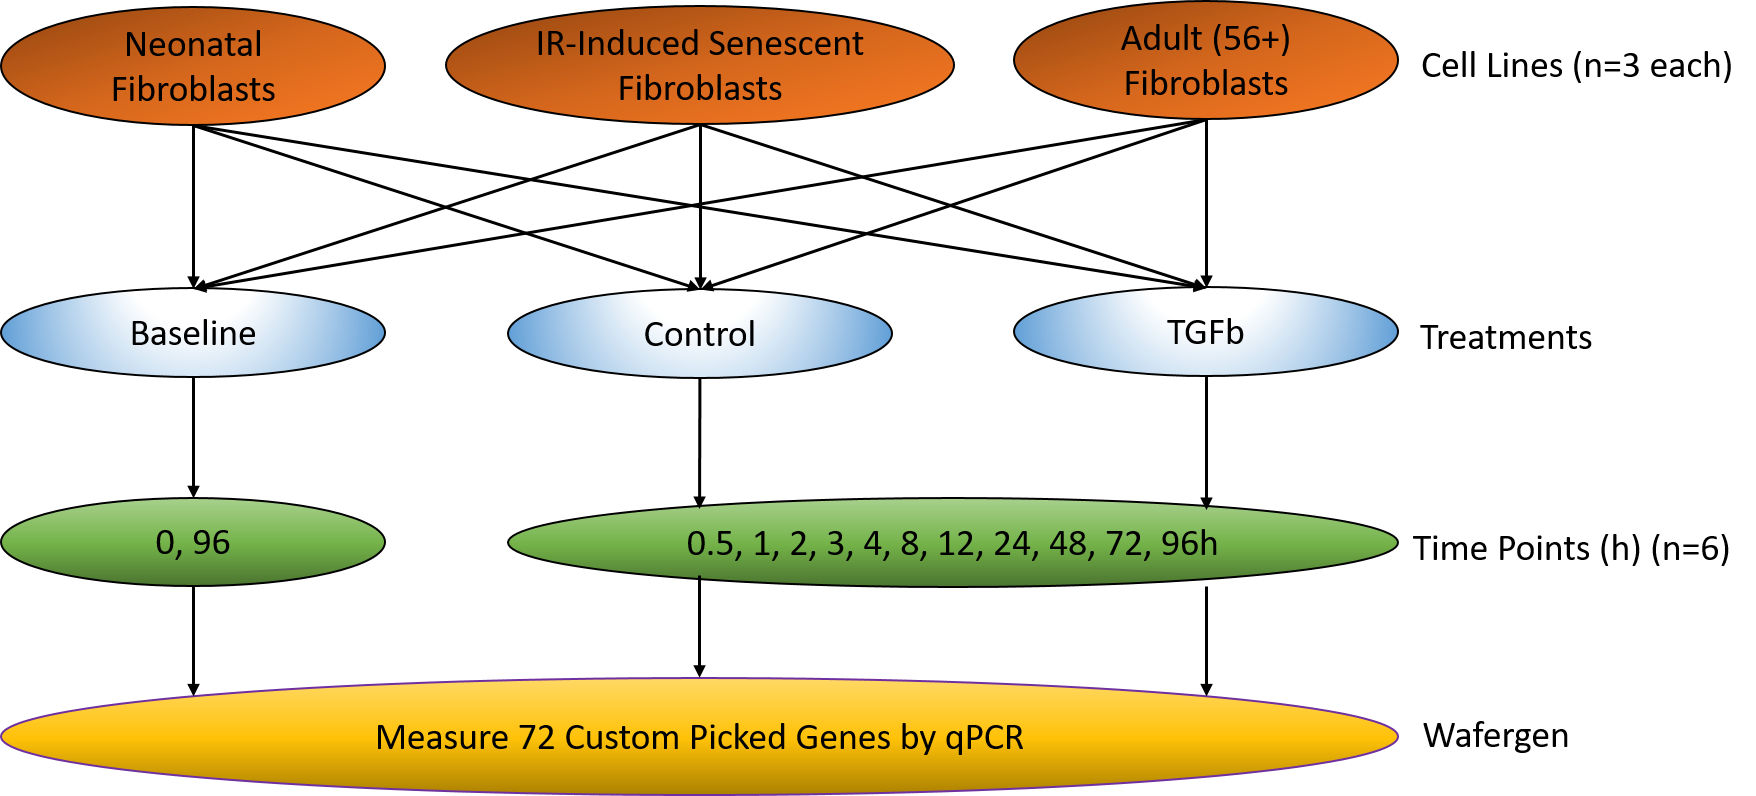
\includegraphics[width=0.8\textwidth]{img/ExperimentDesign}
	\caption{Graphical depiction of experimental design}
	\label{fig:exp_design}
\end{figure}
\subsection{Experiment design}
To identify differences between neonatal, irradiation-induced senescent and adult fibroblasts, the activity of 72 genes were measured over 96h in 3 replicates of each cell group using high throughput qPCR. These measurements were taken both in response to 5ng mL$^{-1}$ \tgf{} reconstituted in 10mM citric acid or 0.1\% BSA in 10mM citric acid as a negative control. The gene chosen were manually selected based on a literature search to be relevant to ECM biology or \tgf{} signalling. The experimental design is depicted in (\cref{fig:exp_design}).
%
\begin{figure}[t]
	\centering
	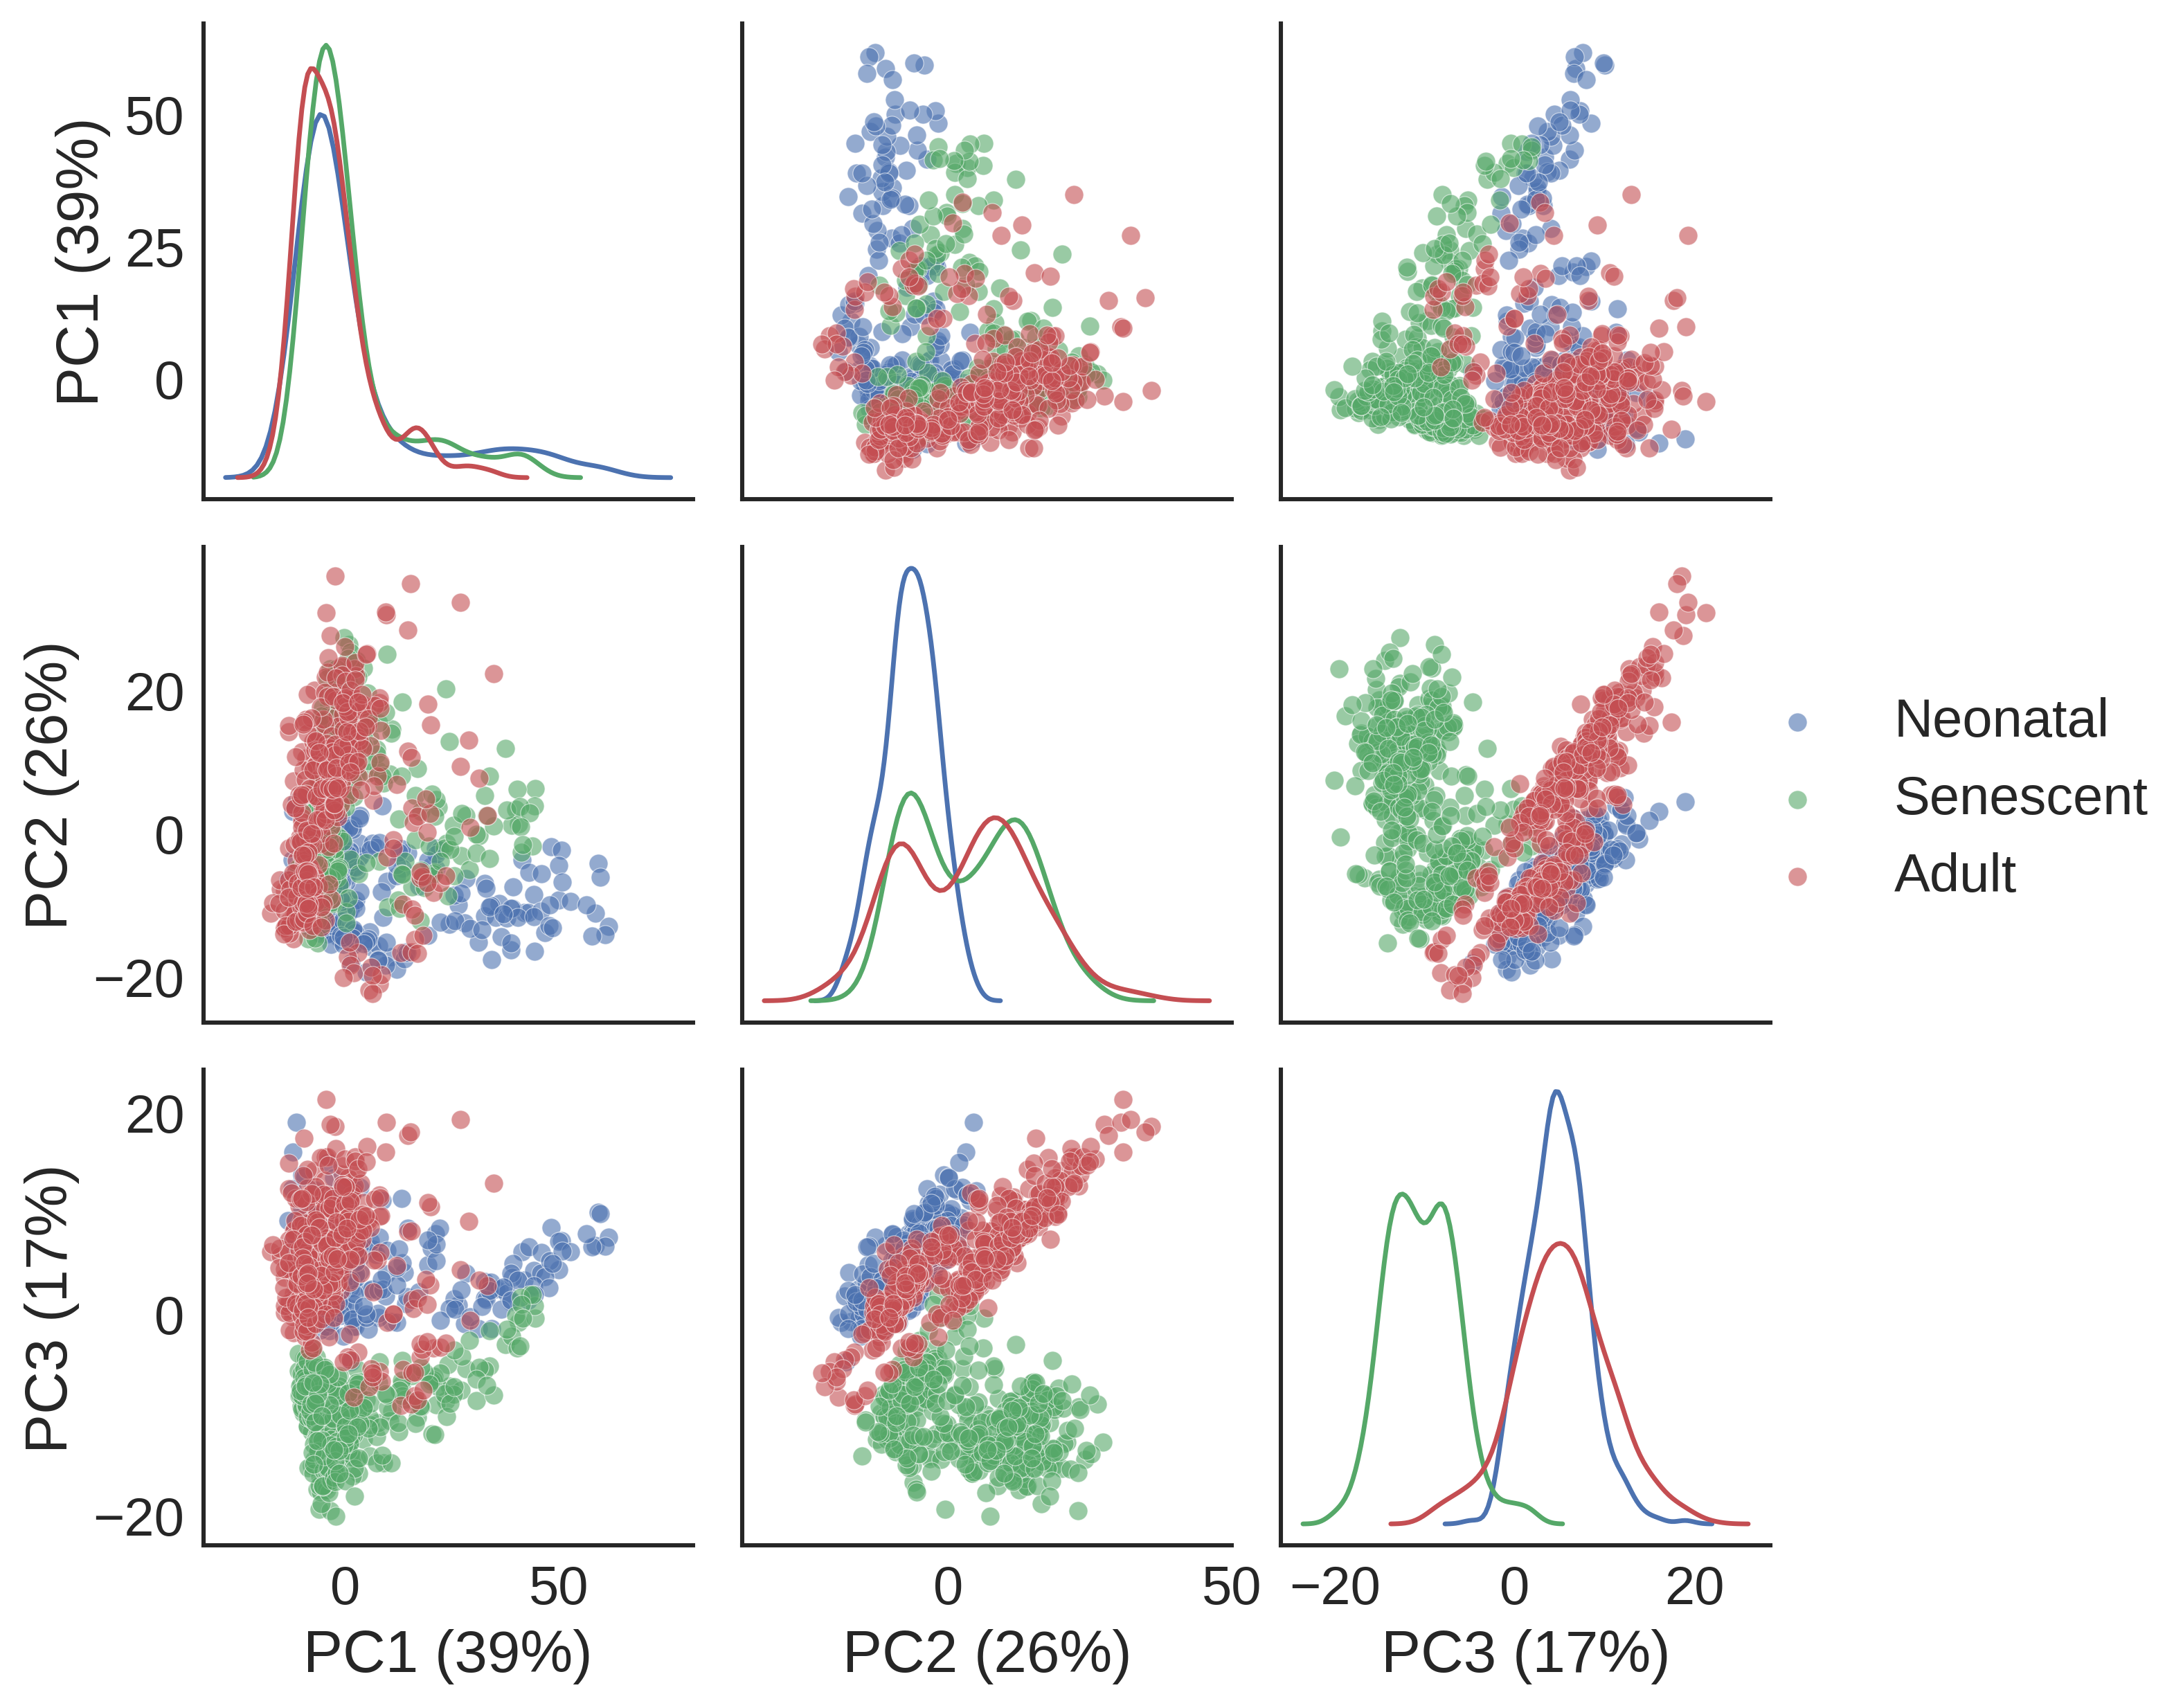
\includegraphics[width=\textwidth]{img/qc/cell_line}
	\caption{Scatter matrix of first three principle components coloured by cell line. Kernel density plots along the diagonal represent the distribution of the relevant principle component.}
	\label{fig:qc:cell_line}
\end{figure}
%
\begin{figure}
	\begin{subfigure}{0.45\linewidth}
		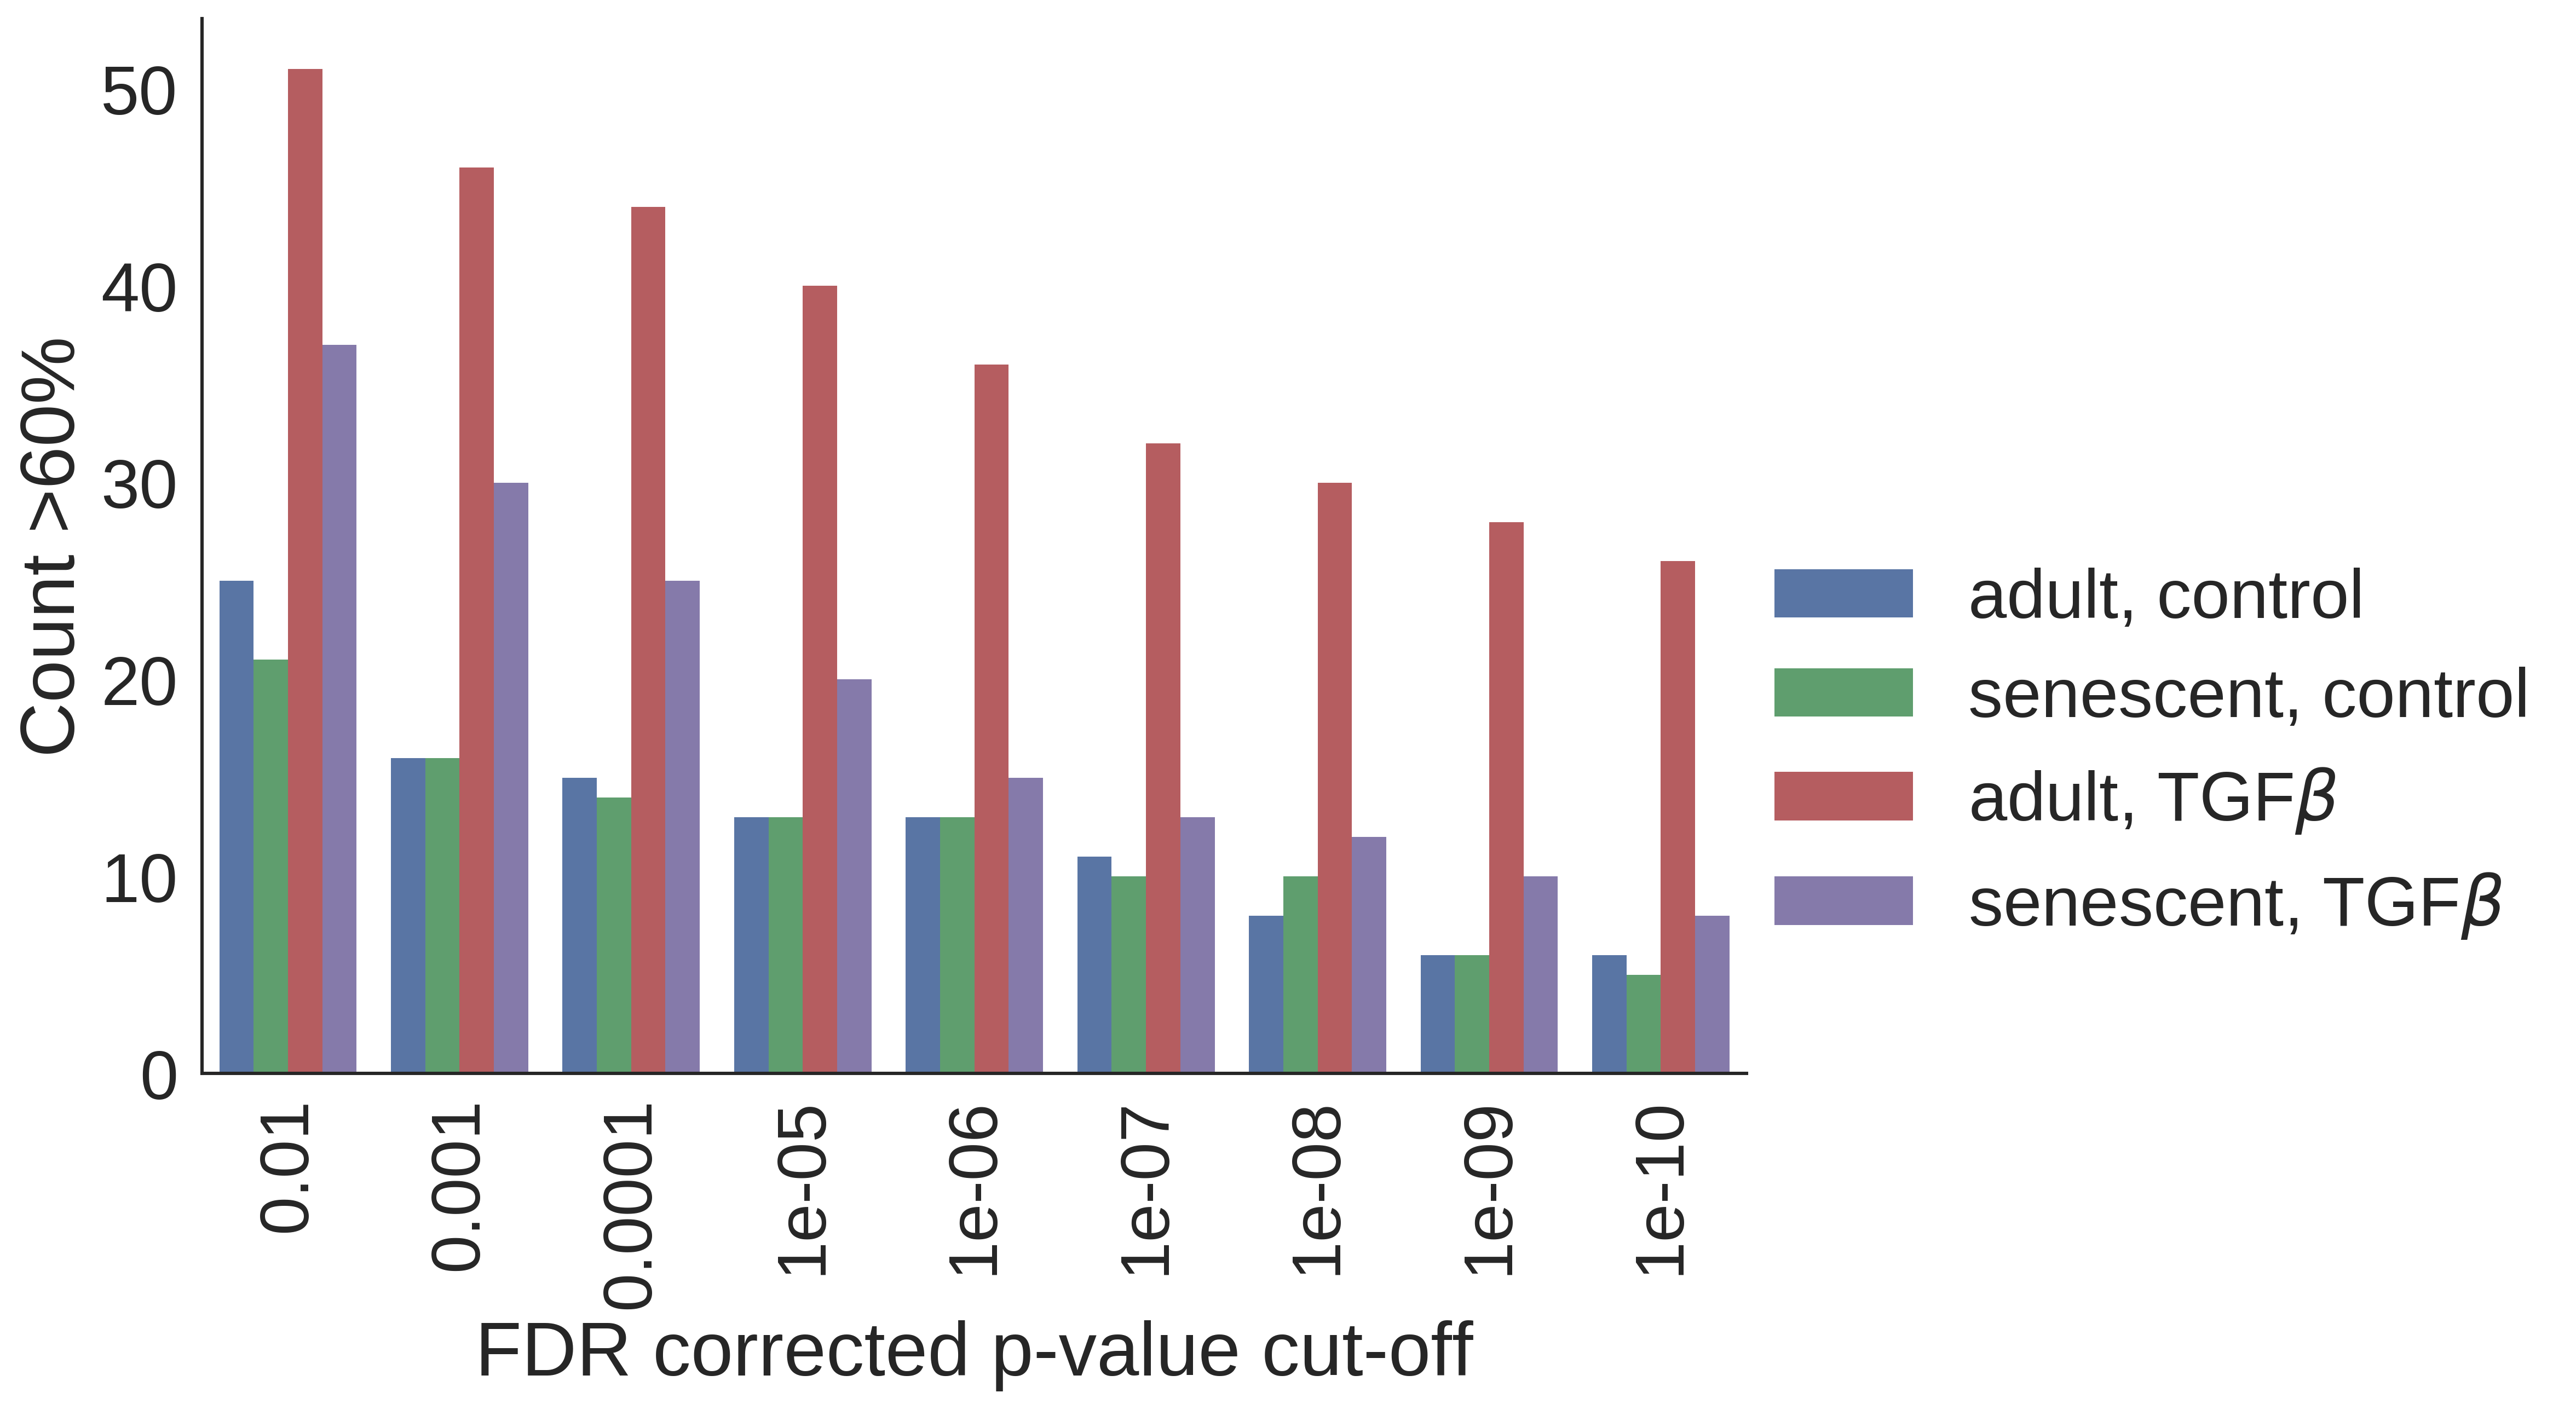
\includegraphics[width=\linewidth]{LIMMA09_2018/SavedObjects/between_pvalue_counts}
		\caption{Between cell lines}
		\label{fig:pvalues:between}
	\end{subfigure}
	\begin{subfigure}{0.45\linewidth}
		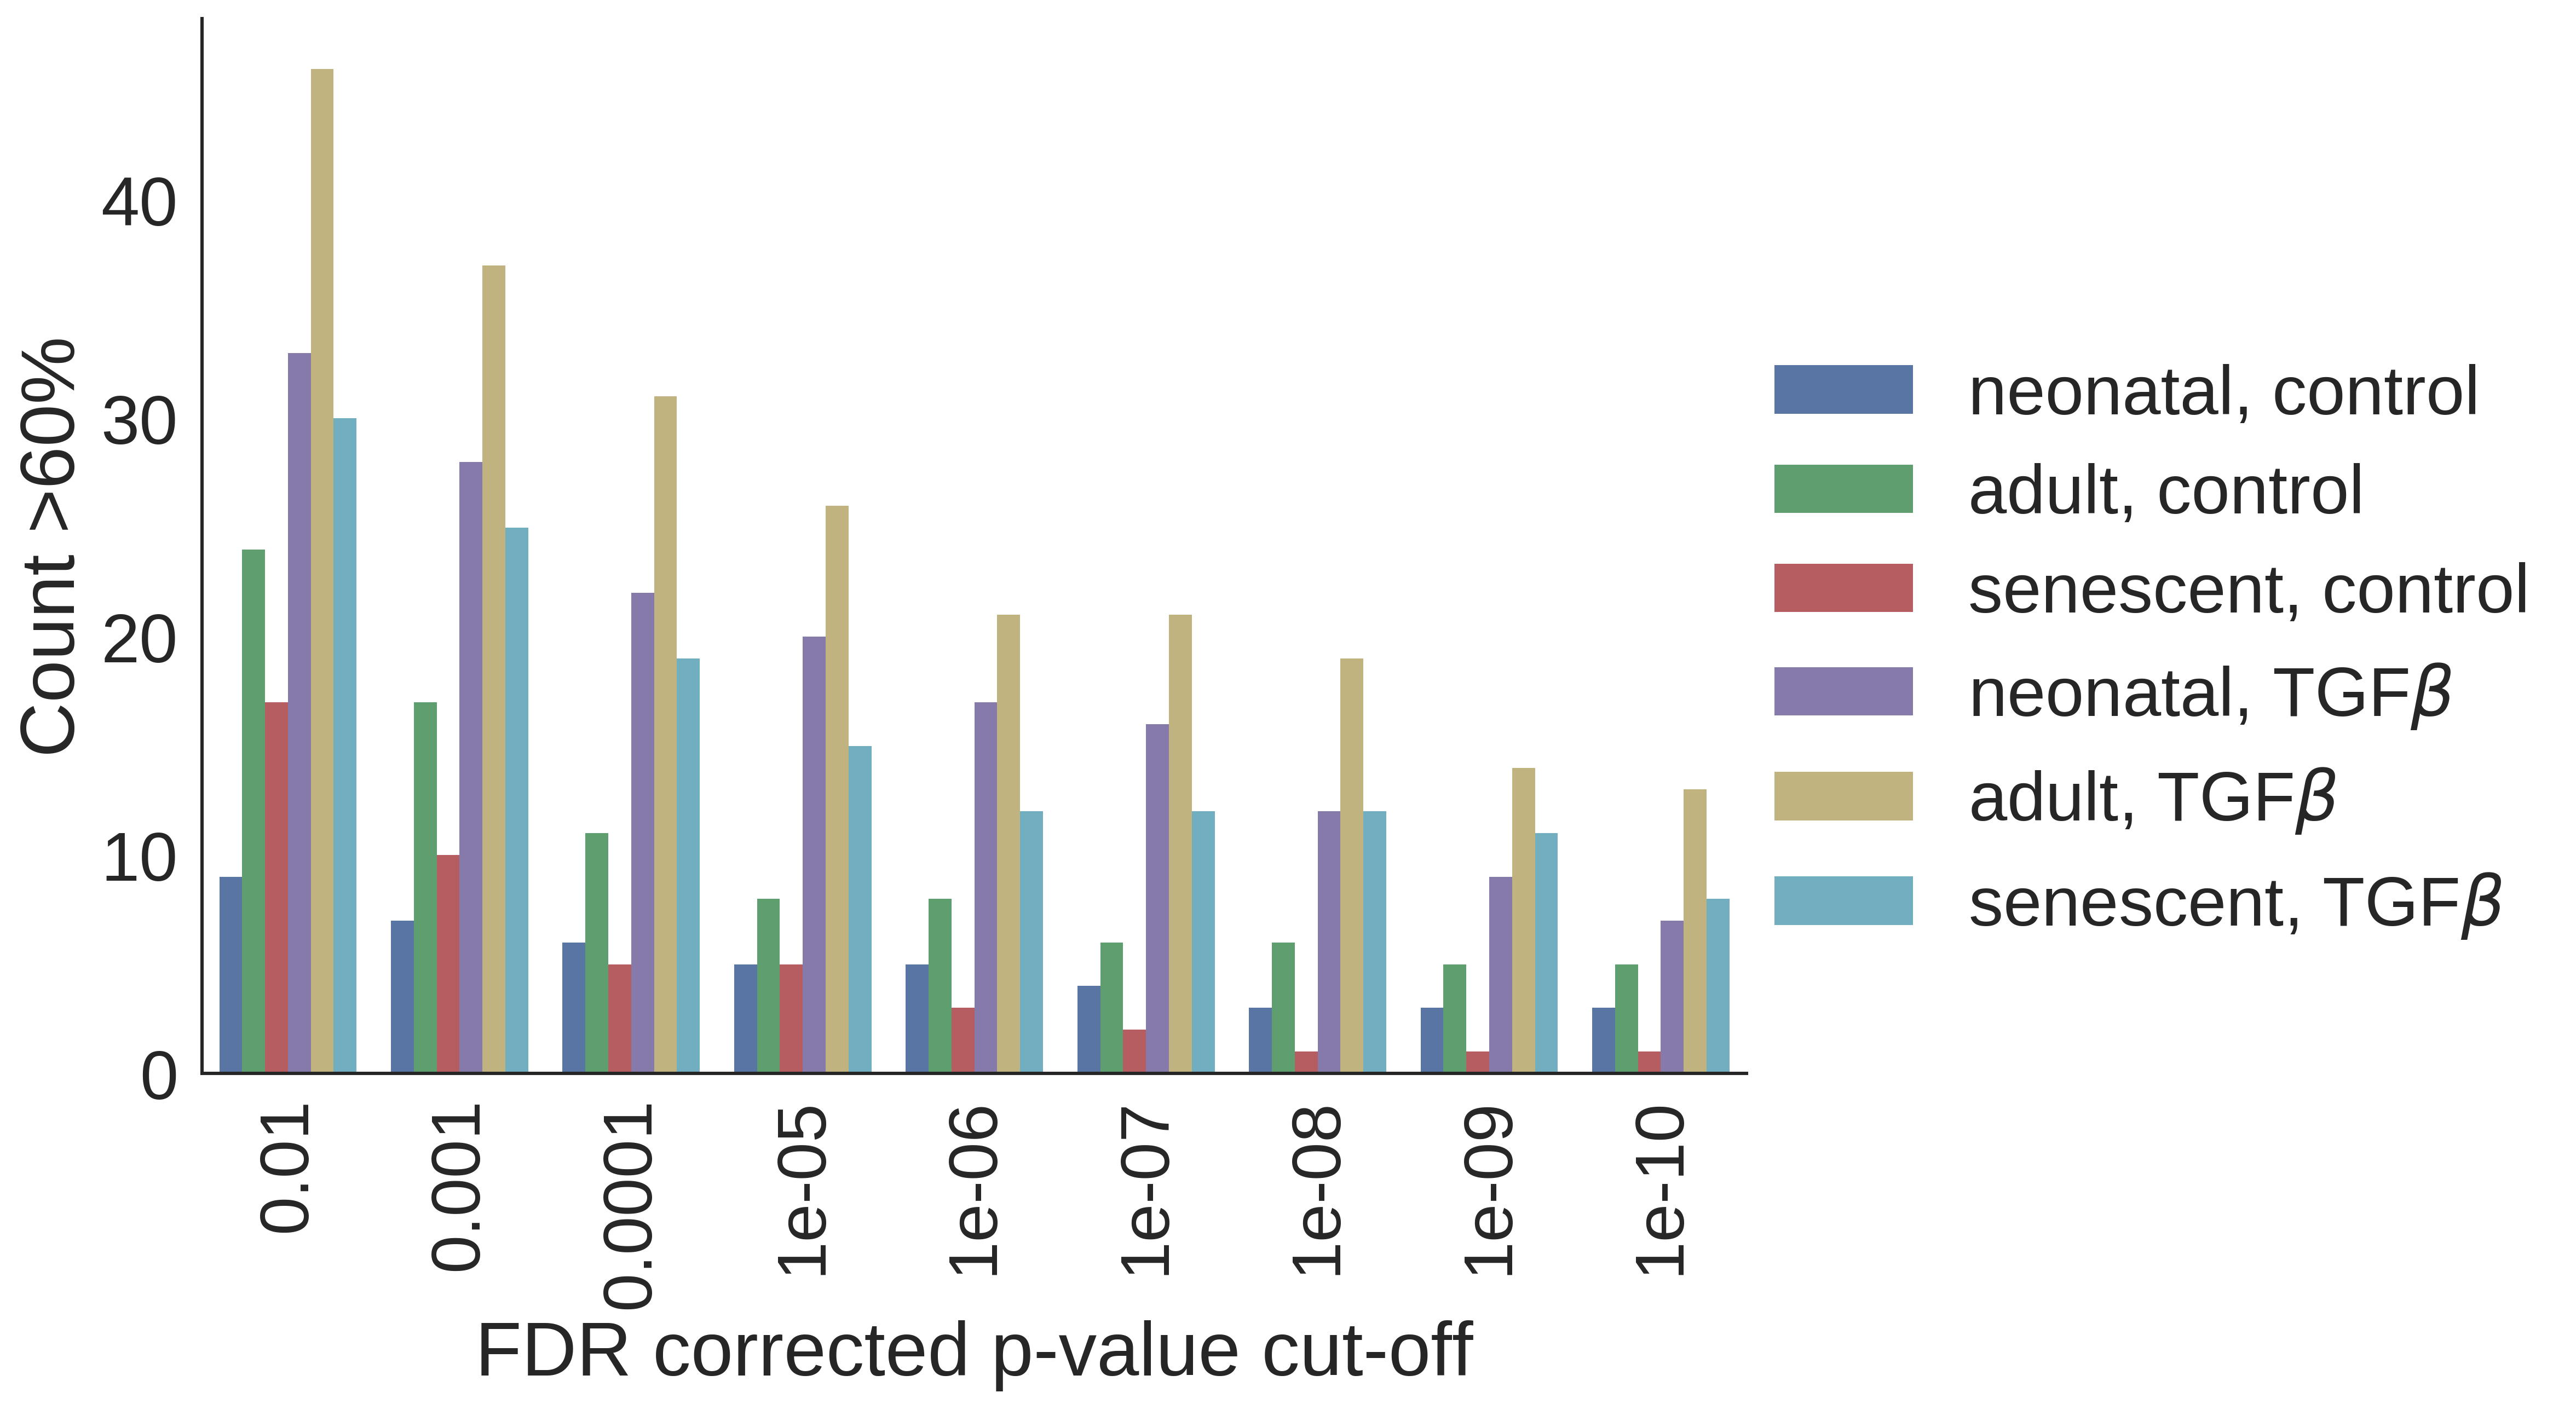
\includegraphics[width=\linewidth]{LIMMA09_2018/SavedObjects/within_pvalue_counts}
		\caption{Within cell lines}
		\label{fig:pvalues:within}
	\end{subfigure}
	\caption{Counts of genes that were differentially expressed in >60\% of LIMMA analyses as a function of p-value for (a) the between groups and (b) within groups comparisons.}
	\label{fig:pvalues}
\end{figure}
%
\subsection{Principle component analysis}
Three primers (IL1A, IL1B and FOSB) were either unreliable or complementary to transcripts present at undetectable quantities and were excluded from further analysis. As a first step in data analysis a principal component analysis (PCA) was conducted to gain confidence in the measurements. The PCA was conducted so each point on the PCA represents one of the 1296 samples. On a PCA, high dimensional data is reduced to a lower dimension whilst maintaining as much of the original variance as possible (ref). Therefore, when two points are close together on the PCA, the underlying data are similar while when two points are distant, the underlying data are very different from one another. By monitoring how the PCA clusters, it is possible to both positively and negatively assess the quality of the experiment. 

To highlight how experimental factors affect PCA clustering, the PCA repeated and visualised 5 times, but coloured by the various experimental factors. These include cell line (\cref{fig:qc:cell_line}), cell ID (\cref{fig:qc:cell_id}), time points (\cref{fig:qc:time_point}), treatment (\cref{fig:qc:treatment}) and by biological replicates (\cref{fig:qc:replicate}). Because the PCA coloured by cell lines, cell IDs, time points and treatments all display clustering while the PCA coloured by replicates does not, this PCA indicates that the data collected is likely representative of the underlying biology. As an alternative interpretation, the PCA shows that is it unlikely that the experiment contains anomalies that confound our understanding of the underlying biology. A scree plot is presented in \cref{fig:qc:scree} and indicates that the first three principal components account for >80\% of variance.

\subsection{Differential expression}
Following the PCA, a differential expression analysis was conducted to investigate whether the time series measurements for each gene was statistically different between` or within cell line groups. The R package LIMMA was used for differential expression analysis. Because our data is dynamic, for each comparison LIMMA was configured to evaluate whether two full time series objects were different from one other using a moderated F-statistic \citep{Ritchie2015, Smyth2004, Smyth2005}. 
\begin{table}[h]
	\centering
	\caption{Table summarising the number of genes per comparison that were differentially expressed with a (FDR corrected) p-value <0.001 in over 60\% of LIMMA analyses per comparison.}
	\begin{tabular}{lll}
		Comparison & Control & \tgf{} \\
		Adult Vs neonatal & 16 & 46 \\
		Senescent Vs neonatal & 16 & 30 \\
		Neonatal Vs neonatal & 7 & 28 \\
		Adult Vs adult & 17 & 37 \\
		Senescent Vs senescent & 10 & 25
	\end{tabular}
	\label{table:stats_summary}
\end{table}
\begin{figure}
	\centering
	\begin{subfigure}{0.45\linewidth}
		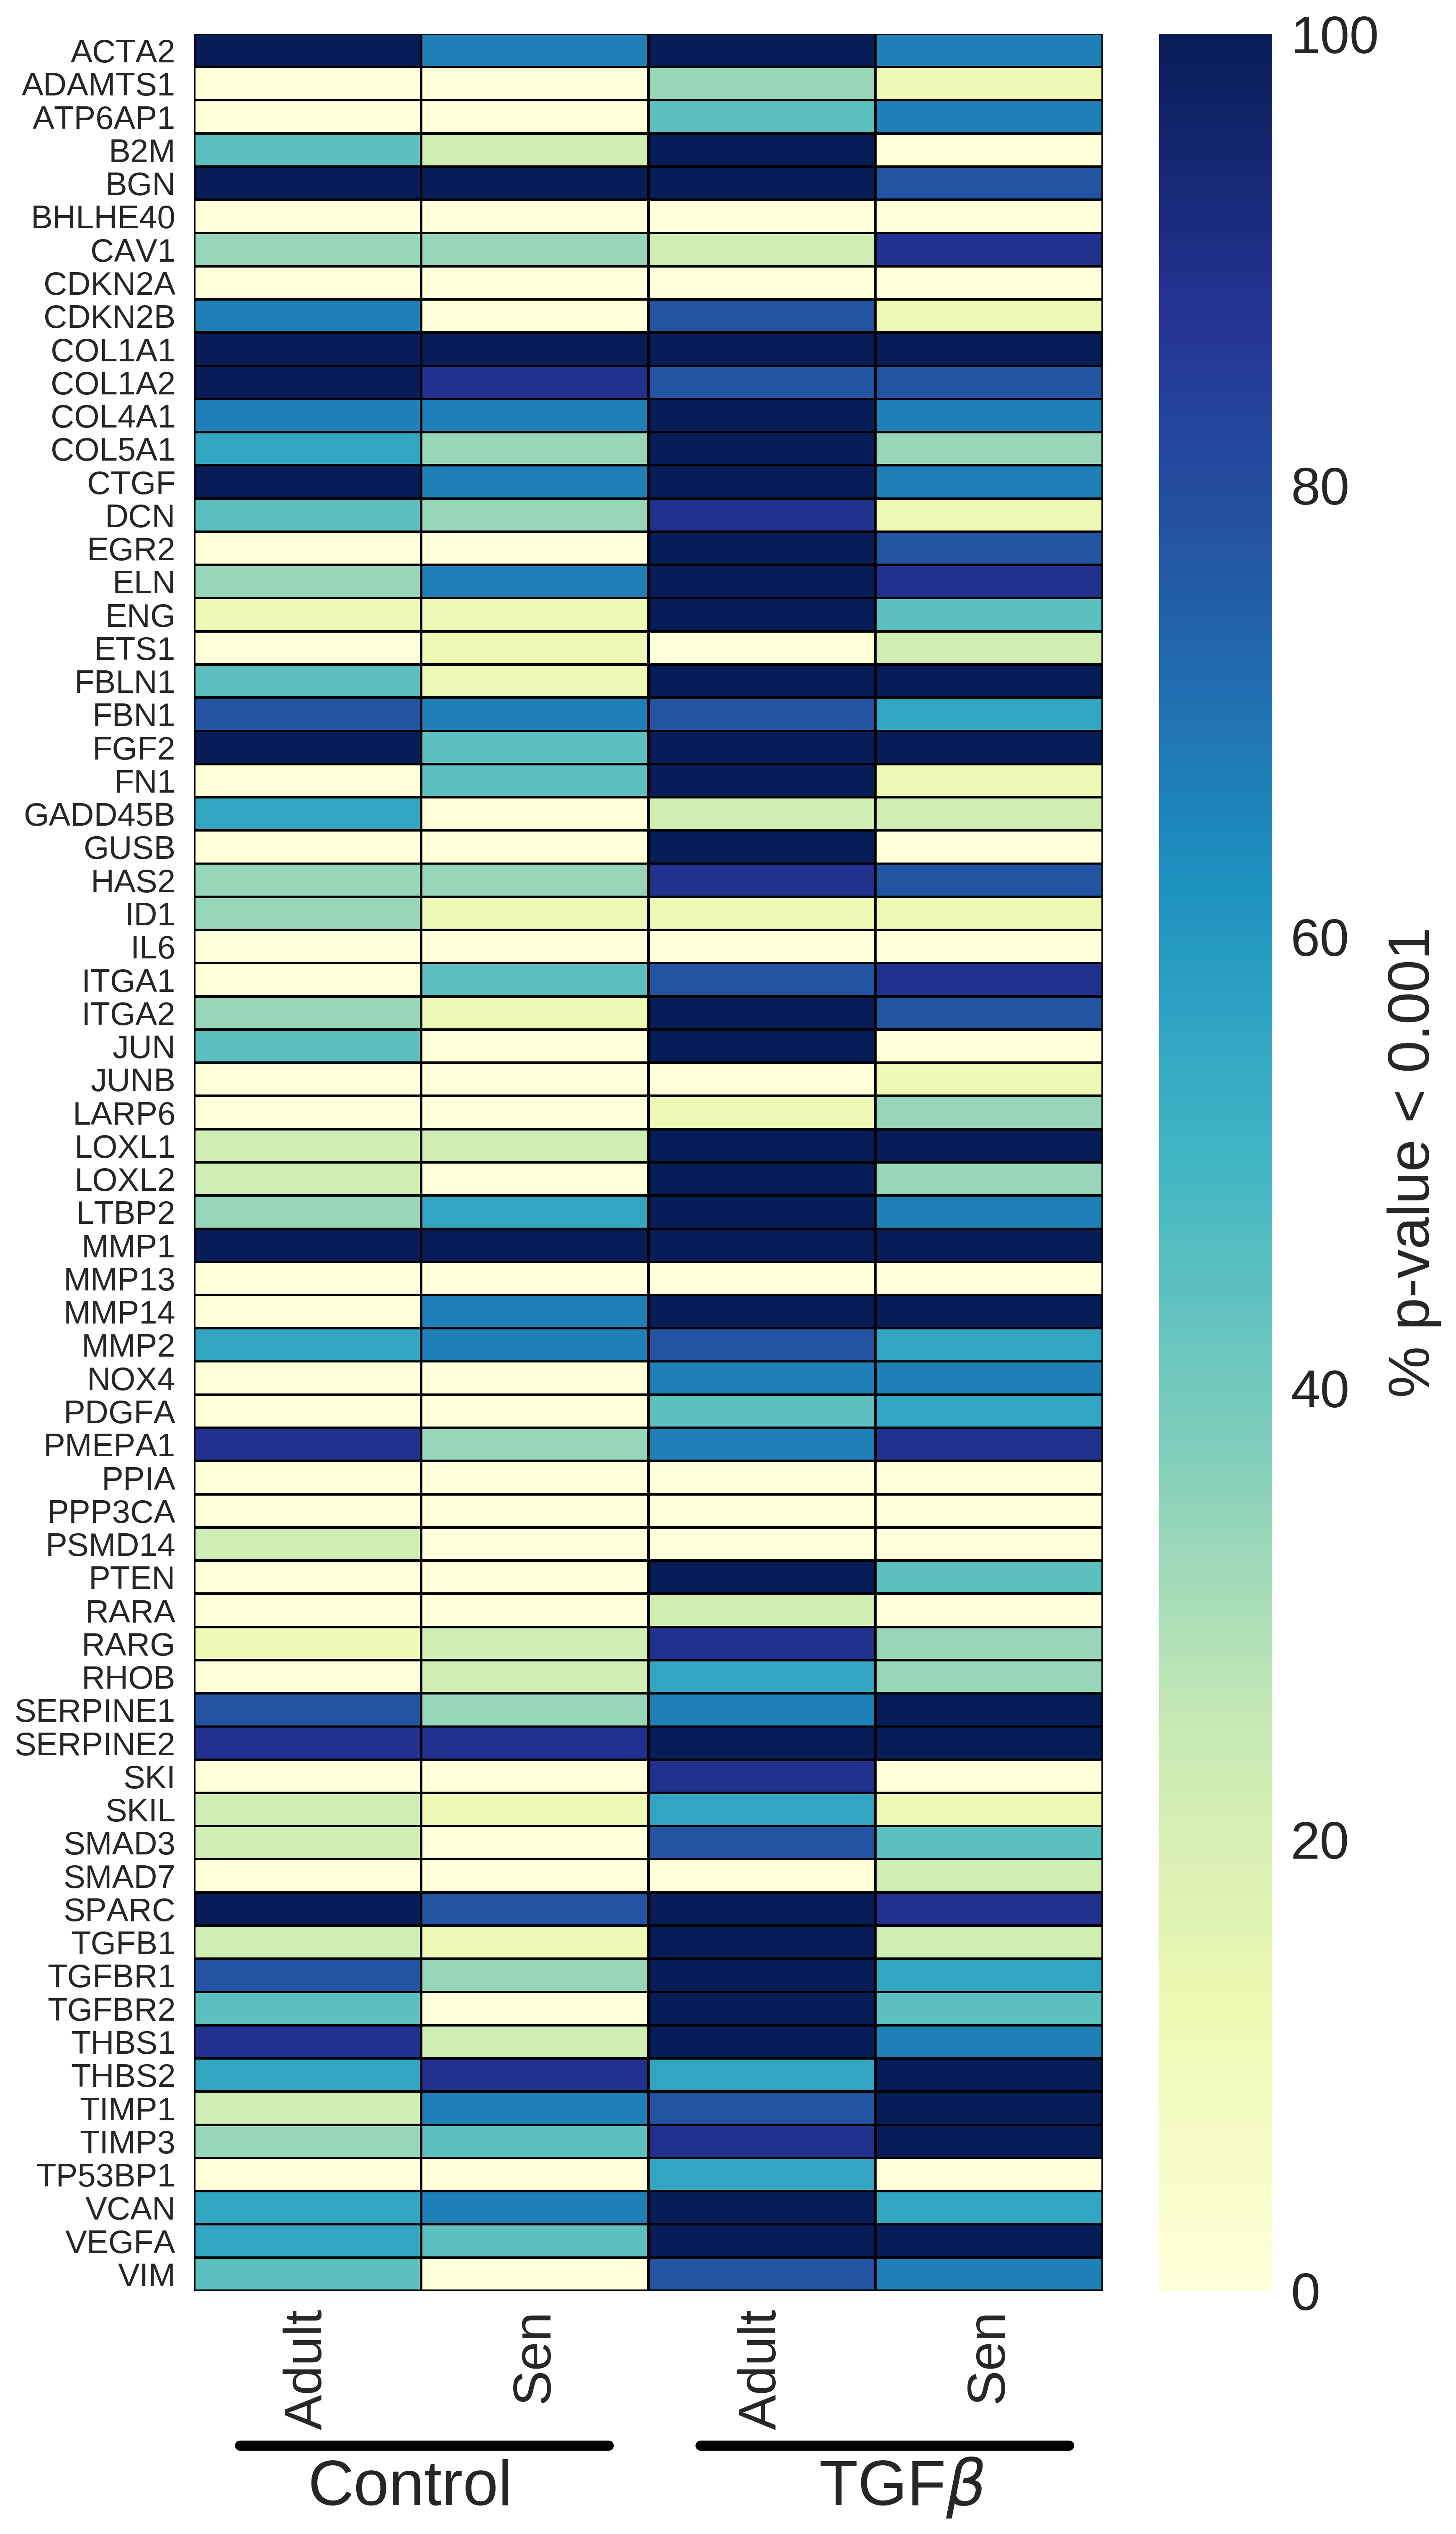
\includegraphics[height=0.7\textheight, width=\linewidth]{LIMMA09_2018/SavedObjects/pval_less_than_0_001/between_heatmap0_001}
		\caption{Between groups comparisons}
		\label{fig:between:heatmap}
	\end{subfigure}
	\begin{subfigure}{0.45\linewidth}
		%		\centering
		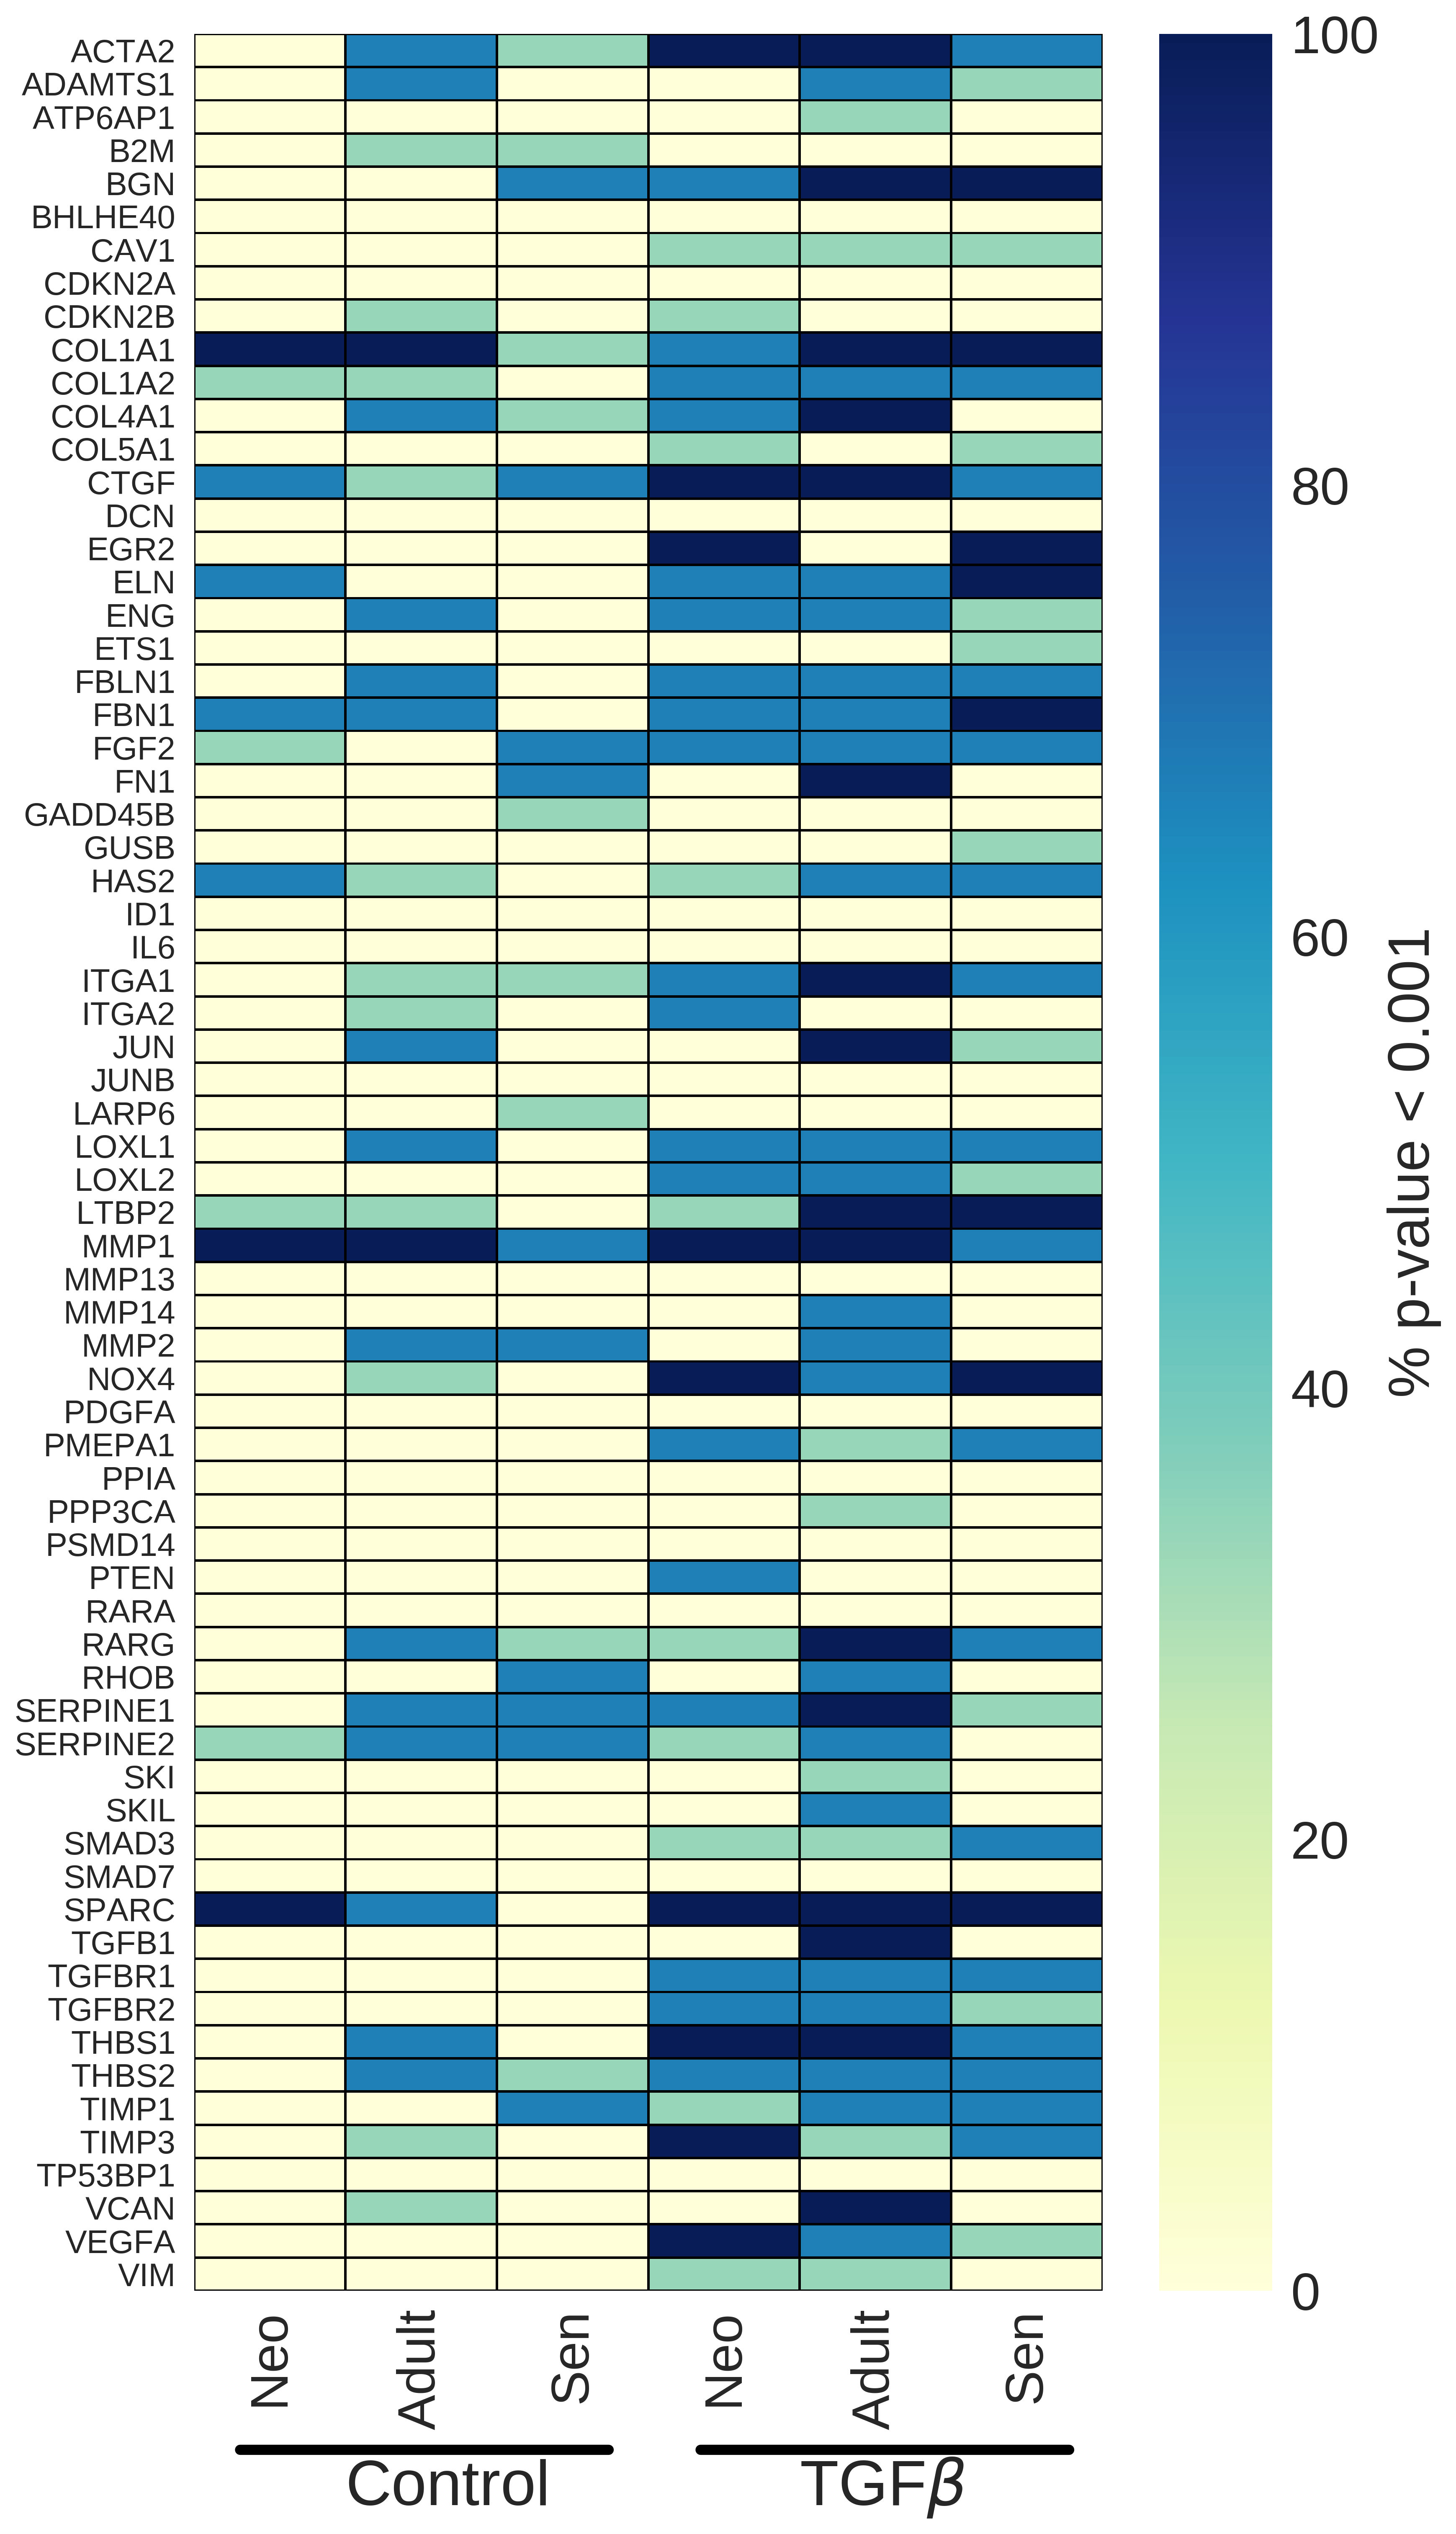
\includegraphics[height=0.7\textheight,width=\linewidth]{LIMMA09_2018/SavedObjects/pval_less_than_0_001/within_heatmap_0_001}
		\caption{Within groups comparisons}
		\label{fig:within:heatmap}
	\end{subfigure}
	\caption{Differential expression analysis for (a) between groups comparisons and (b) within groups comparisons. Colours indicate the percentage of the time of all combinations (9 for between groups and 3 for within groups) of LIMMA analysis conducted that a time series was differentially expressed with a FDR corrected p-value >0.001. }
	\label{fig:heatmap}
\end{figure}
%
\begin{figure}[p]
	\captionsetup[subfigure]{justification=centering}
	\begin{minipage}{0.9\textwidth}
		\centering
		\begin{subfigure}[b]{0.45\textwidth}
			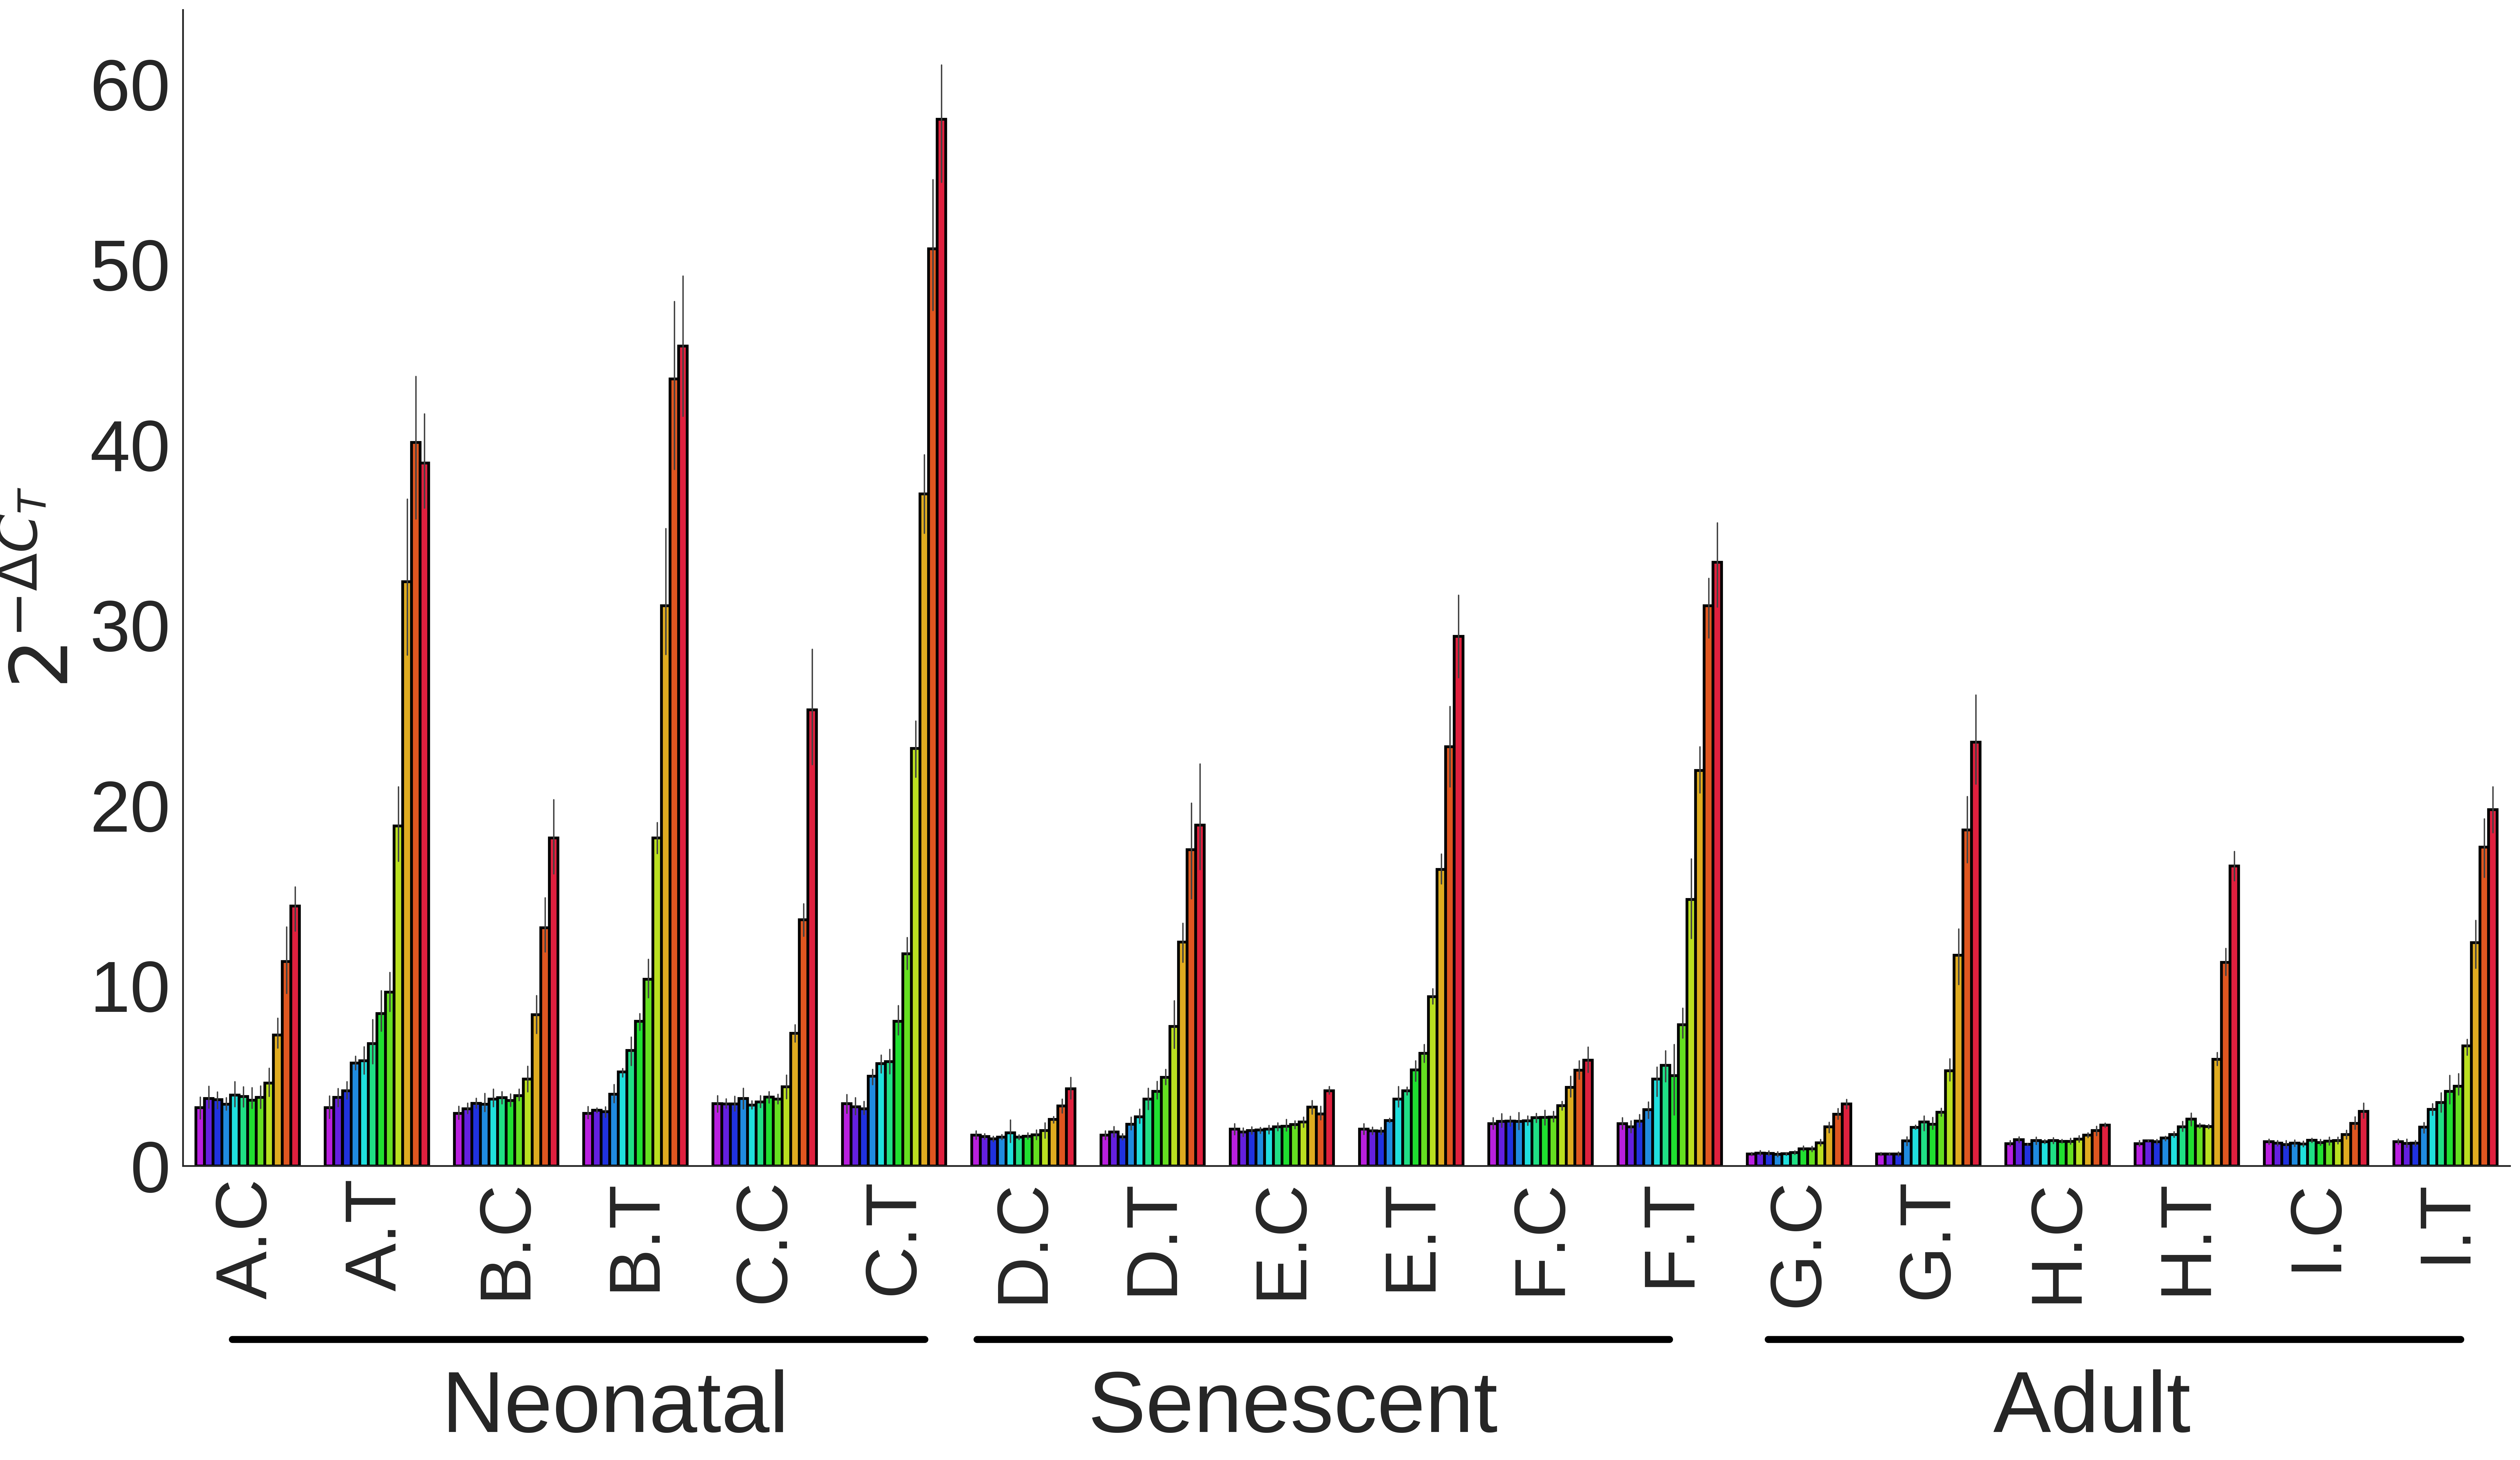
\includegraphics[width=\textwidth]{img/dct_for_publication_no_legend/COL1A1}
			\caption{COL1A1}\label{COL1A1}
		\end{subfigure}\hspace*{\fill}
		\begin{subfigure}[b]{0.45\textwidth}
			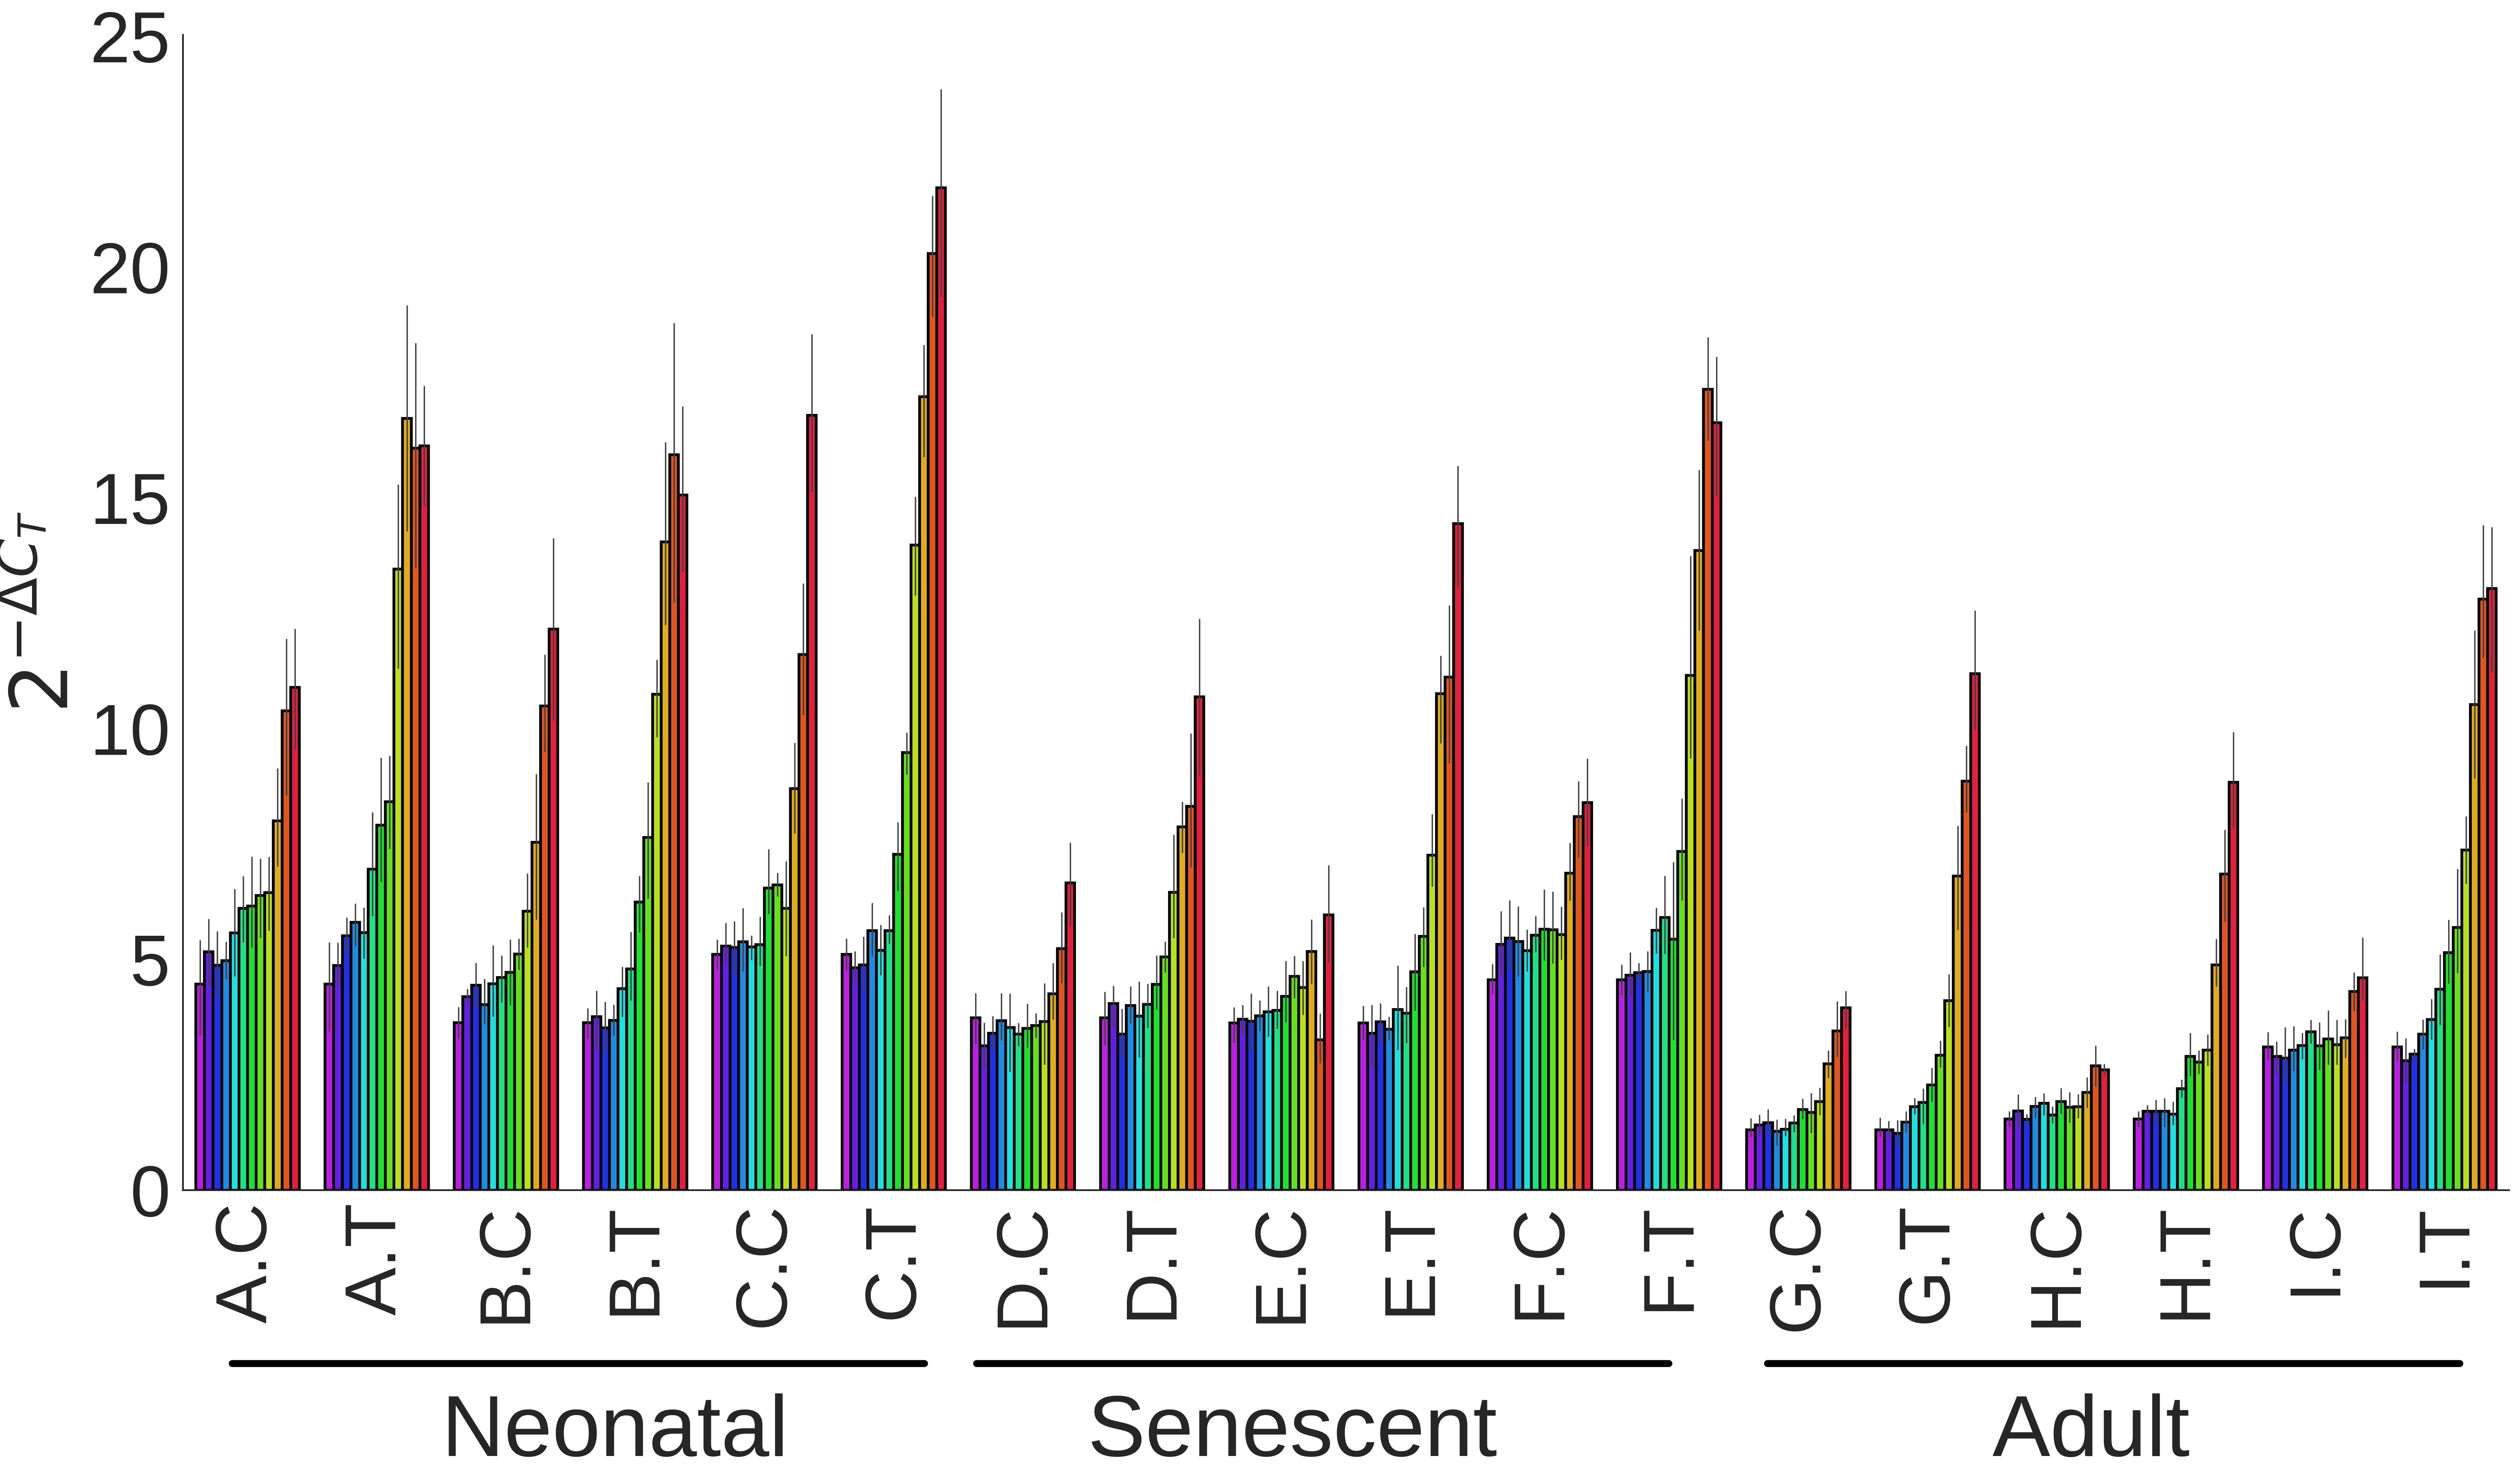
\includegraphics[width=\textwidth]{img/dct_for_publication_no_legend/COL1A2}
			\caption{COL1A2}\label{COL1A2}
		\end{subfigure}\hspace*{\fill}
		
		\begin{subfigure}[b]{0.45\textwidth}
			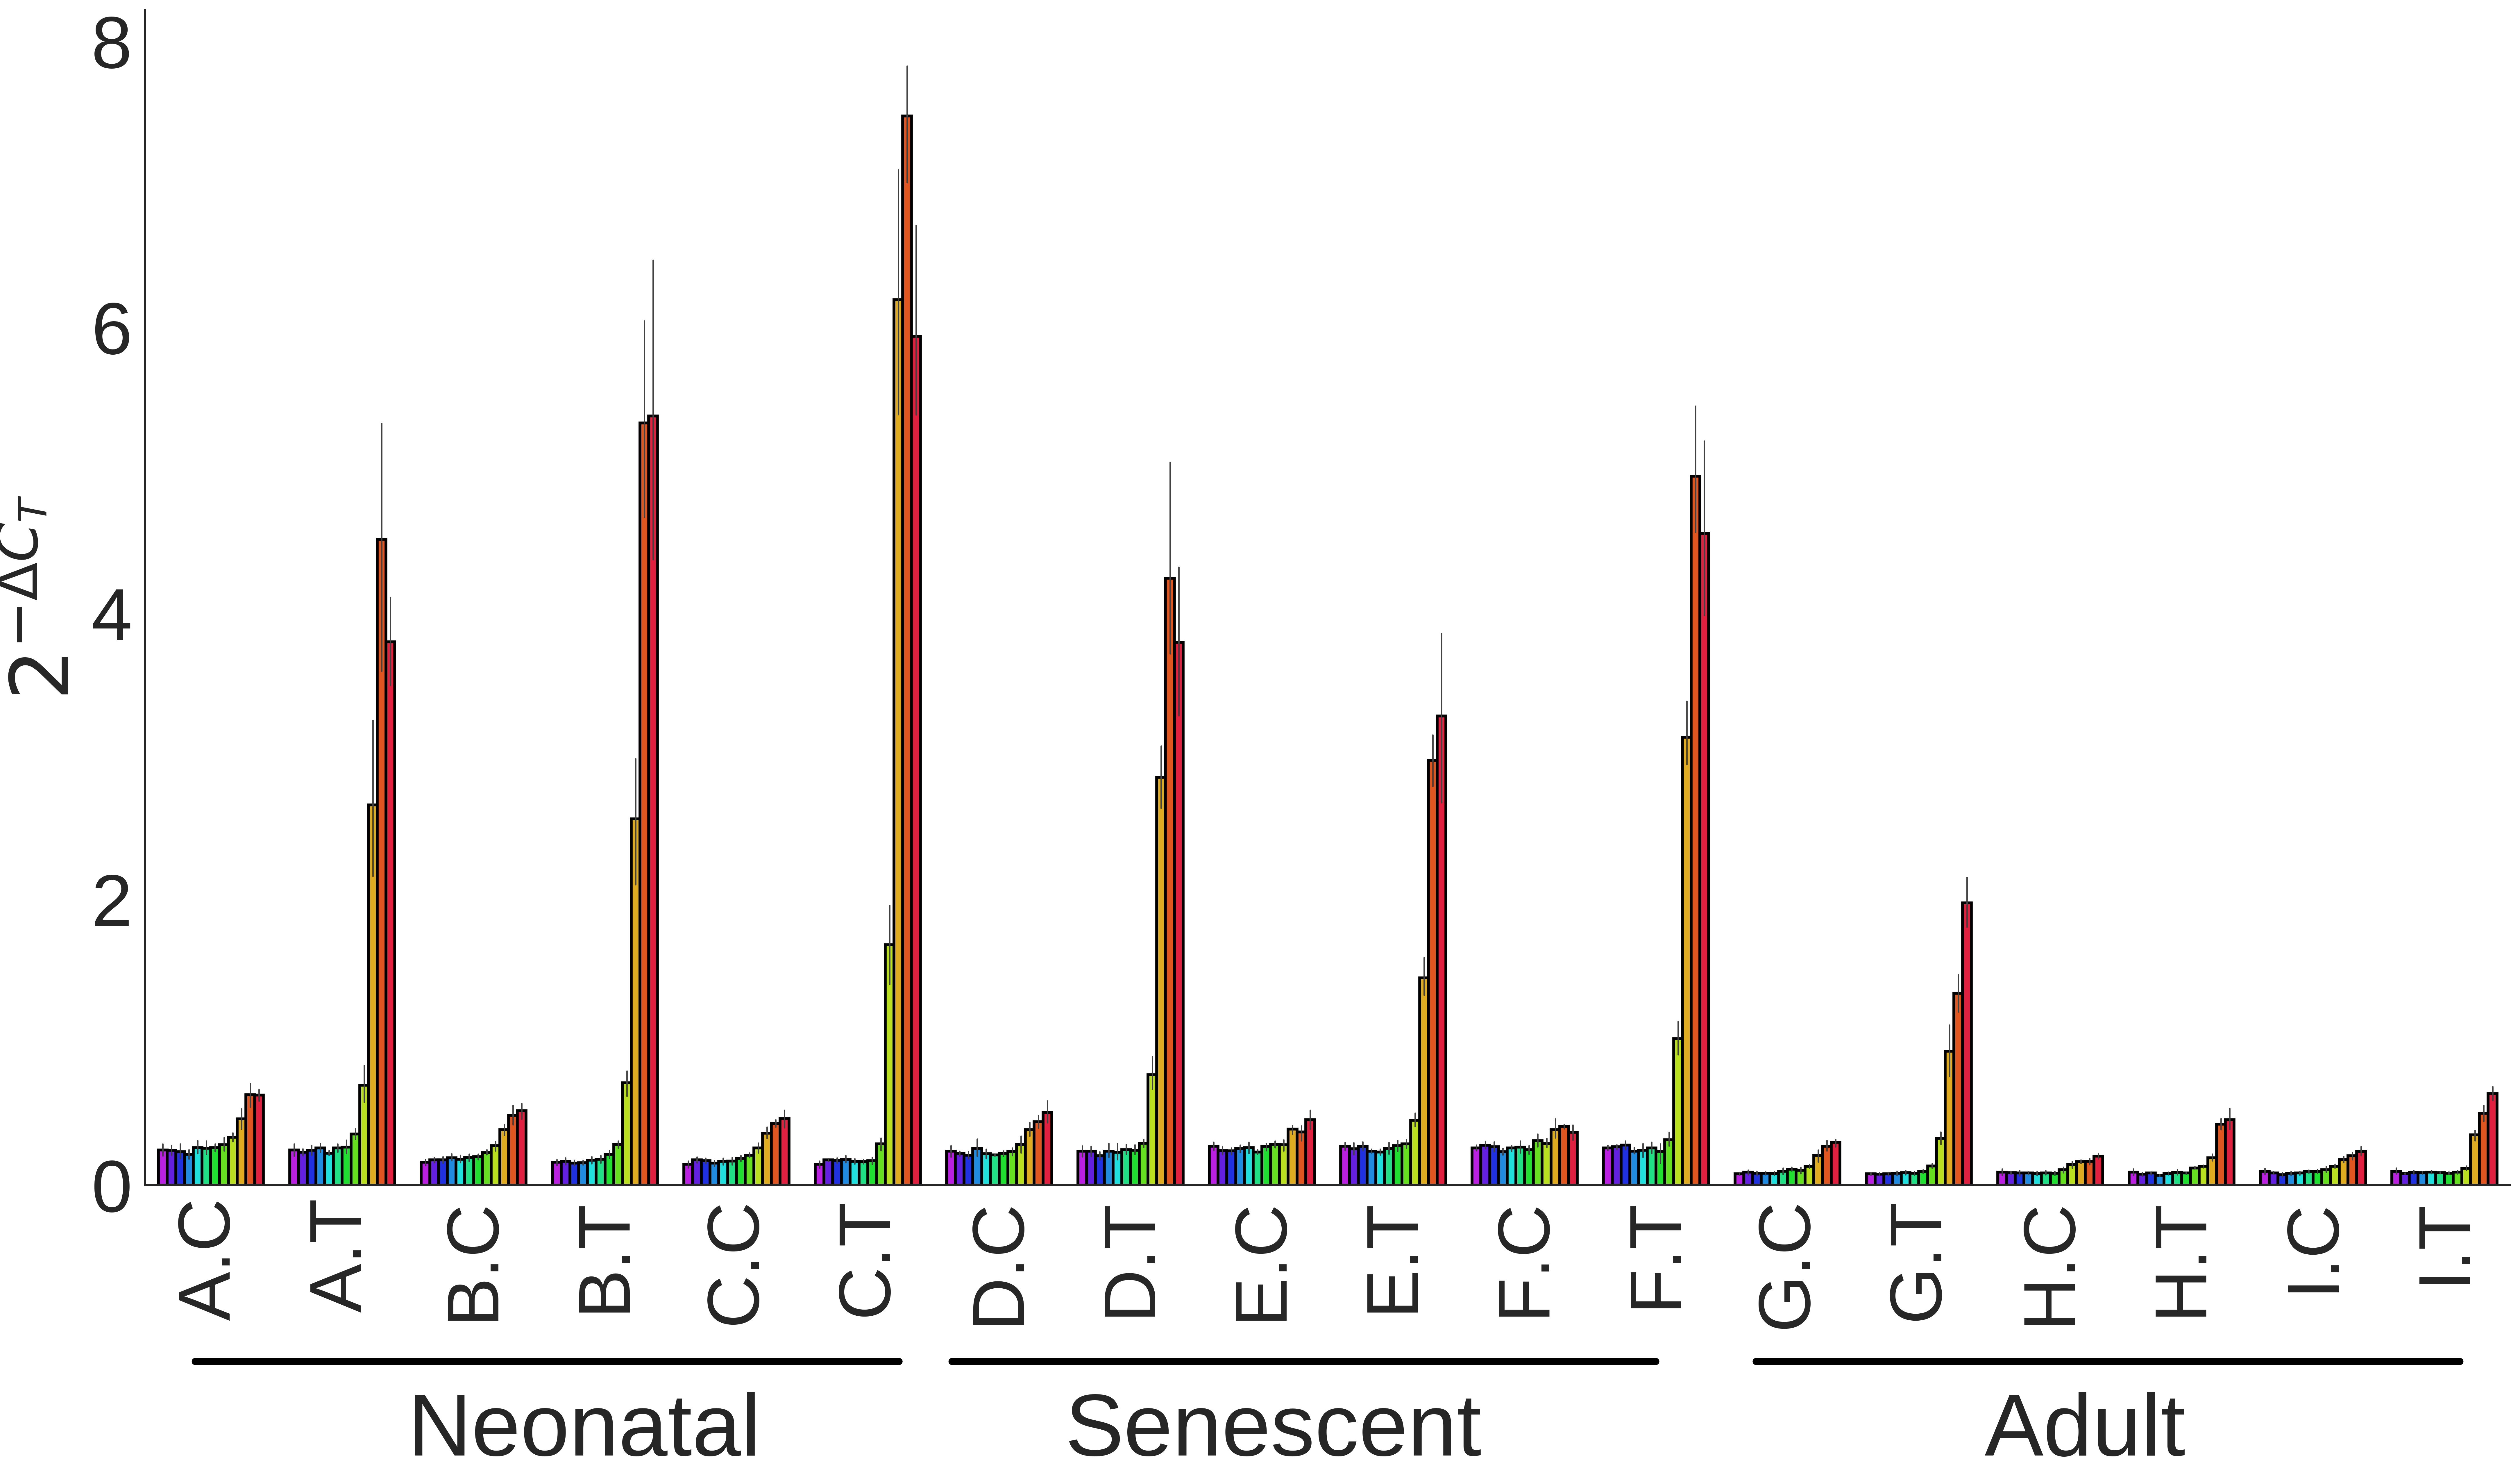
\includegraphics[width=\textwidth]{img/dct_for_publication_no_legend/ACTA2}
			\caption{ACTA2}\label{ACTA2}
		\end{subfigure}\hspace*{\fill}
		\begin{subfigure}[b]{0.45\textwidth}
			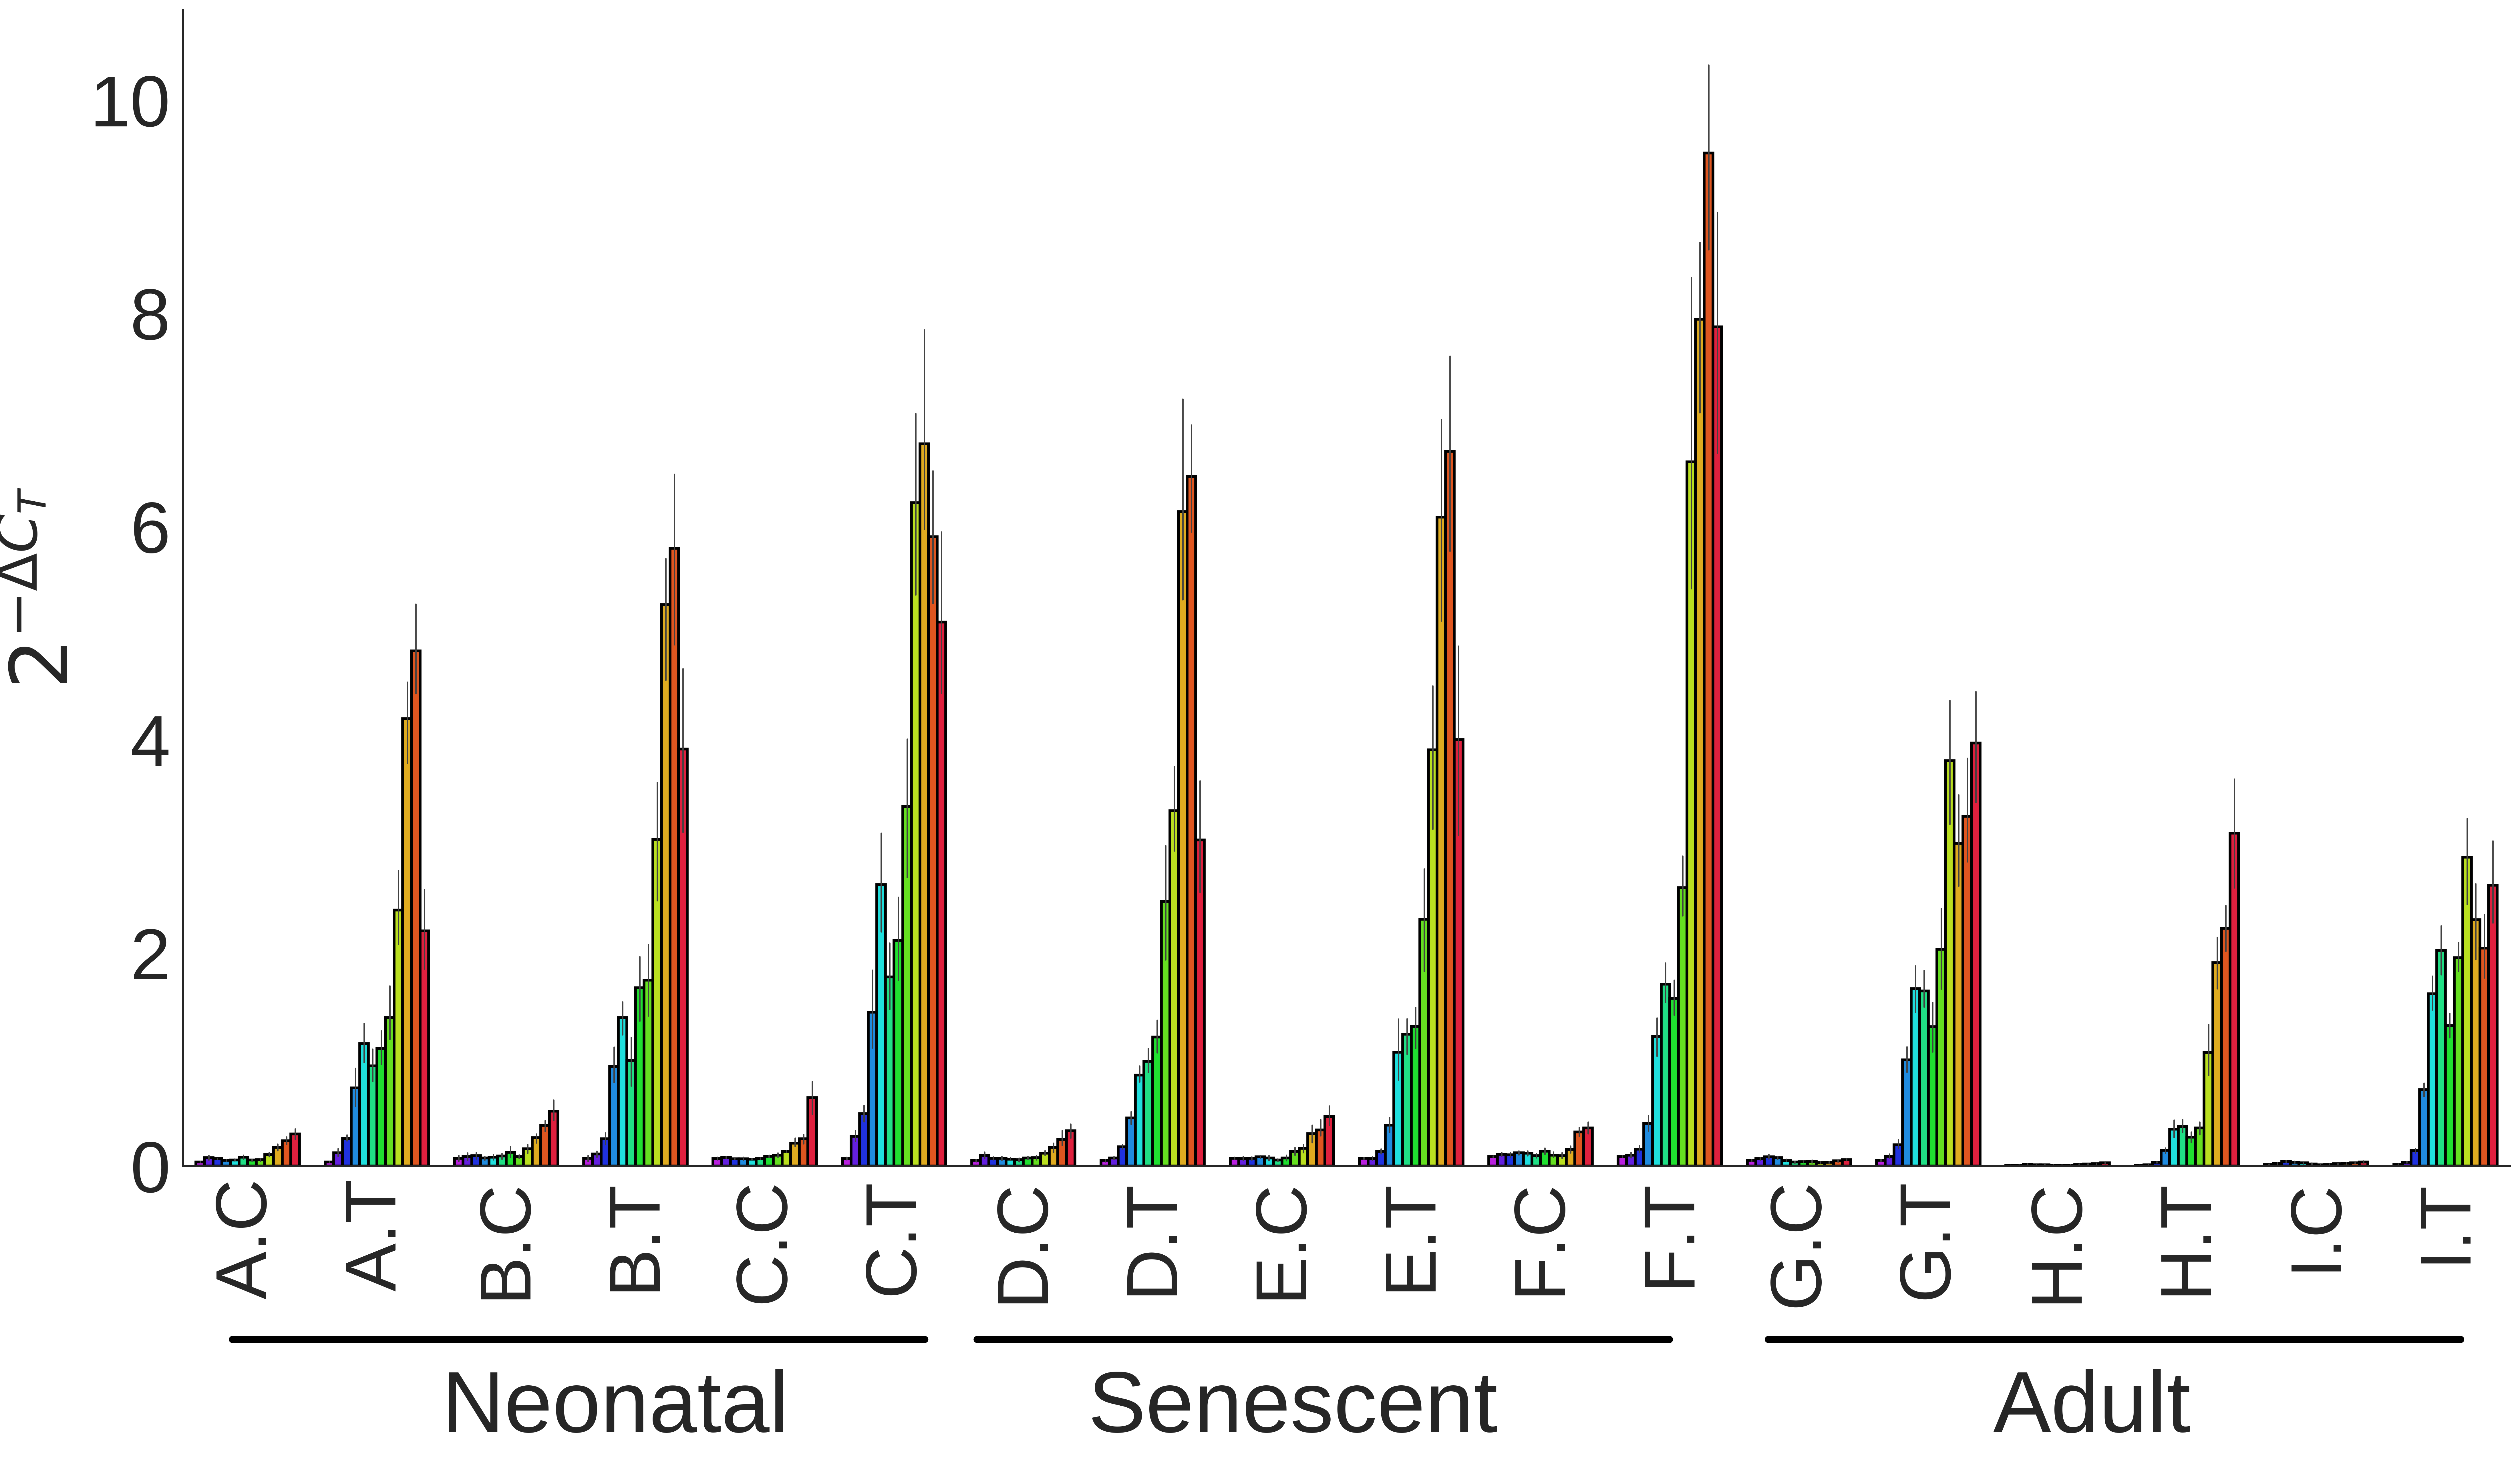
\includegraphics[width=\textwidth]{img/dct_for_publication_no_legend/CTGF}
			\caption{CTGF}\label{CTGF}
		\end{subfigure}\hspace*{\fill}
		
		\begin{subfigure}[b]{0.45\textwidth}
			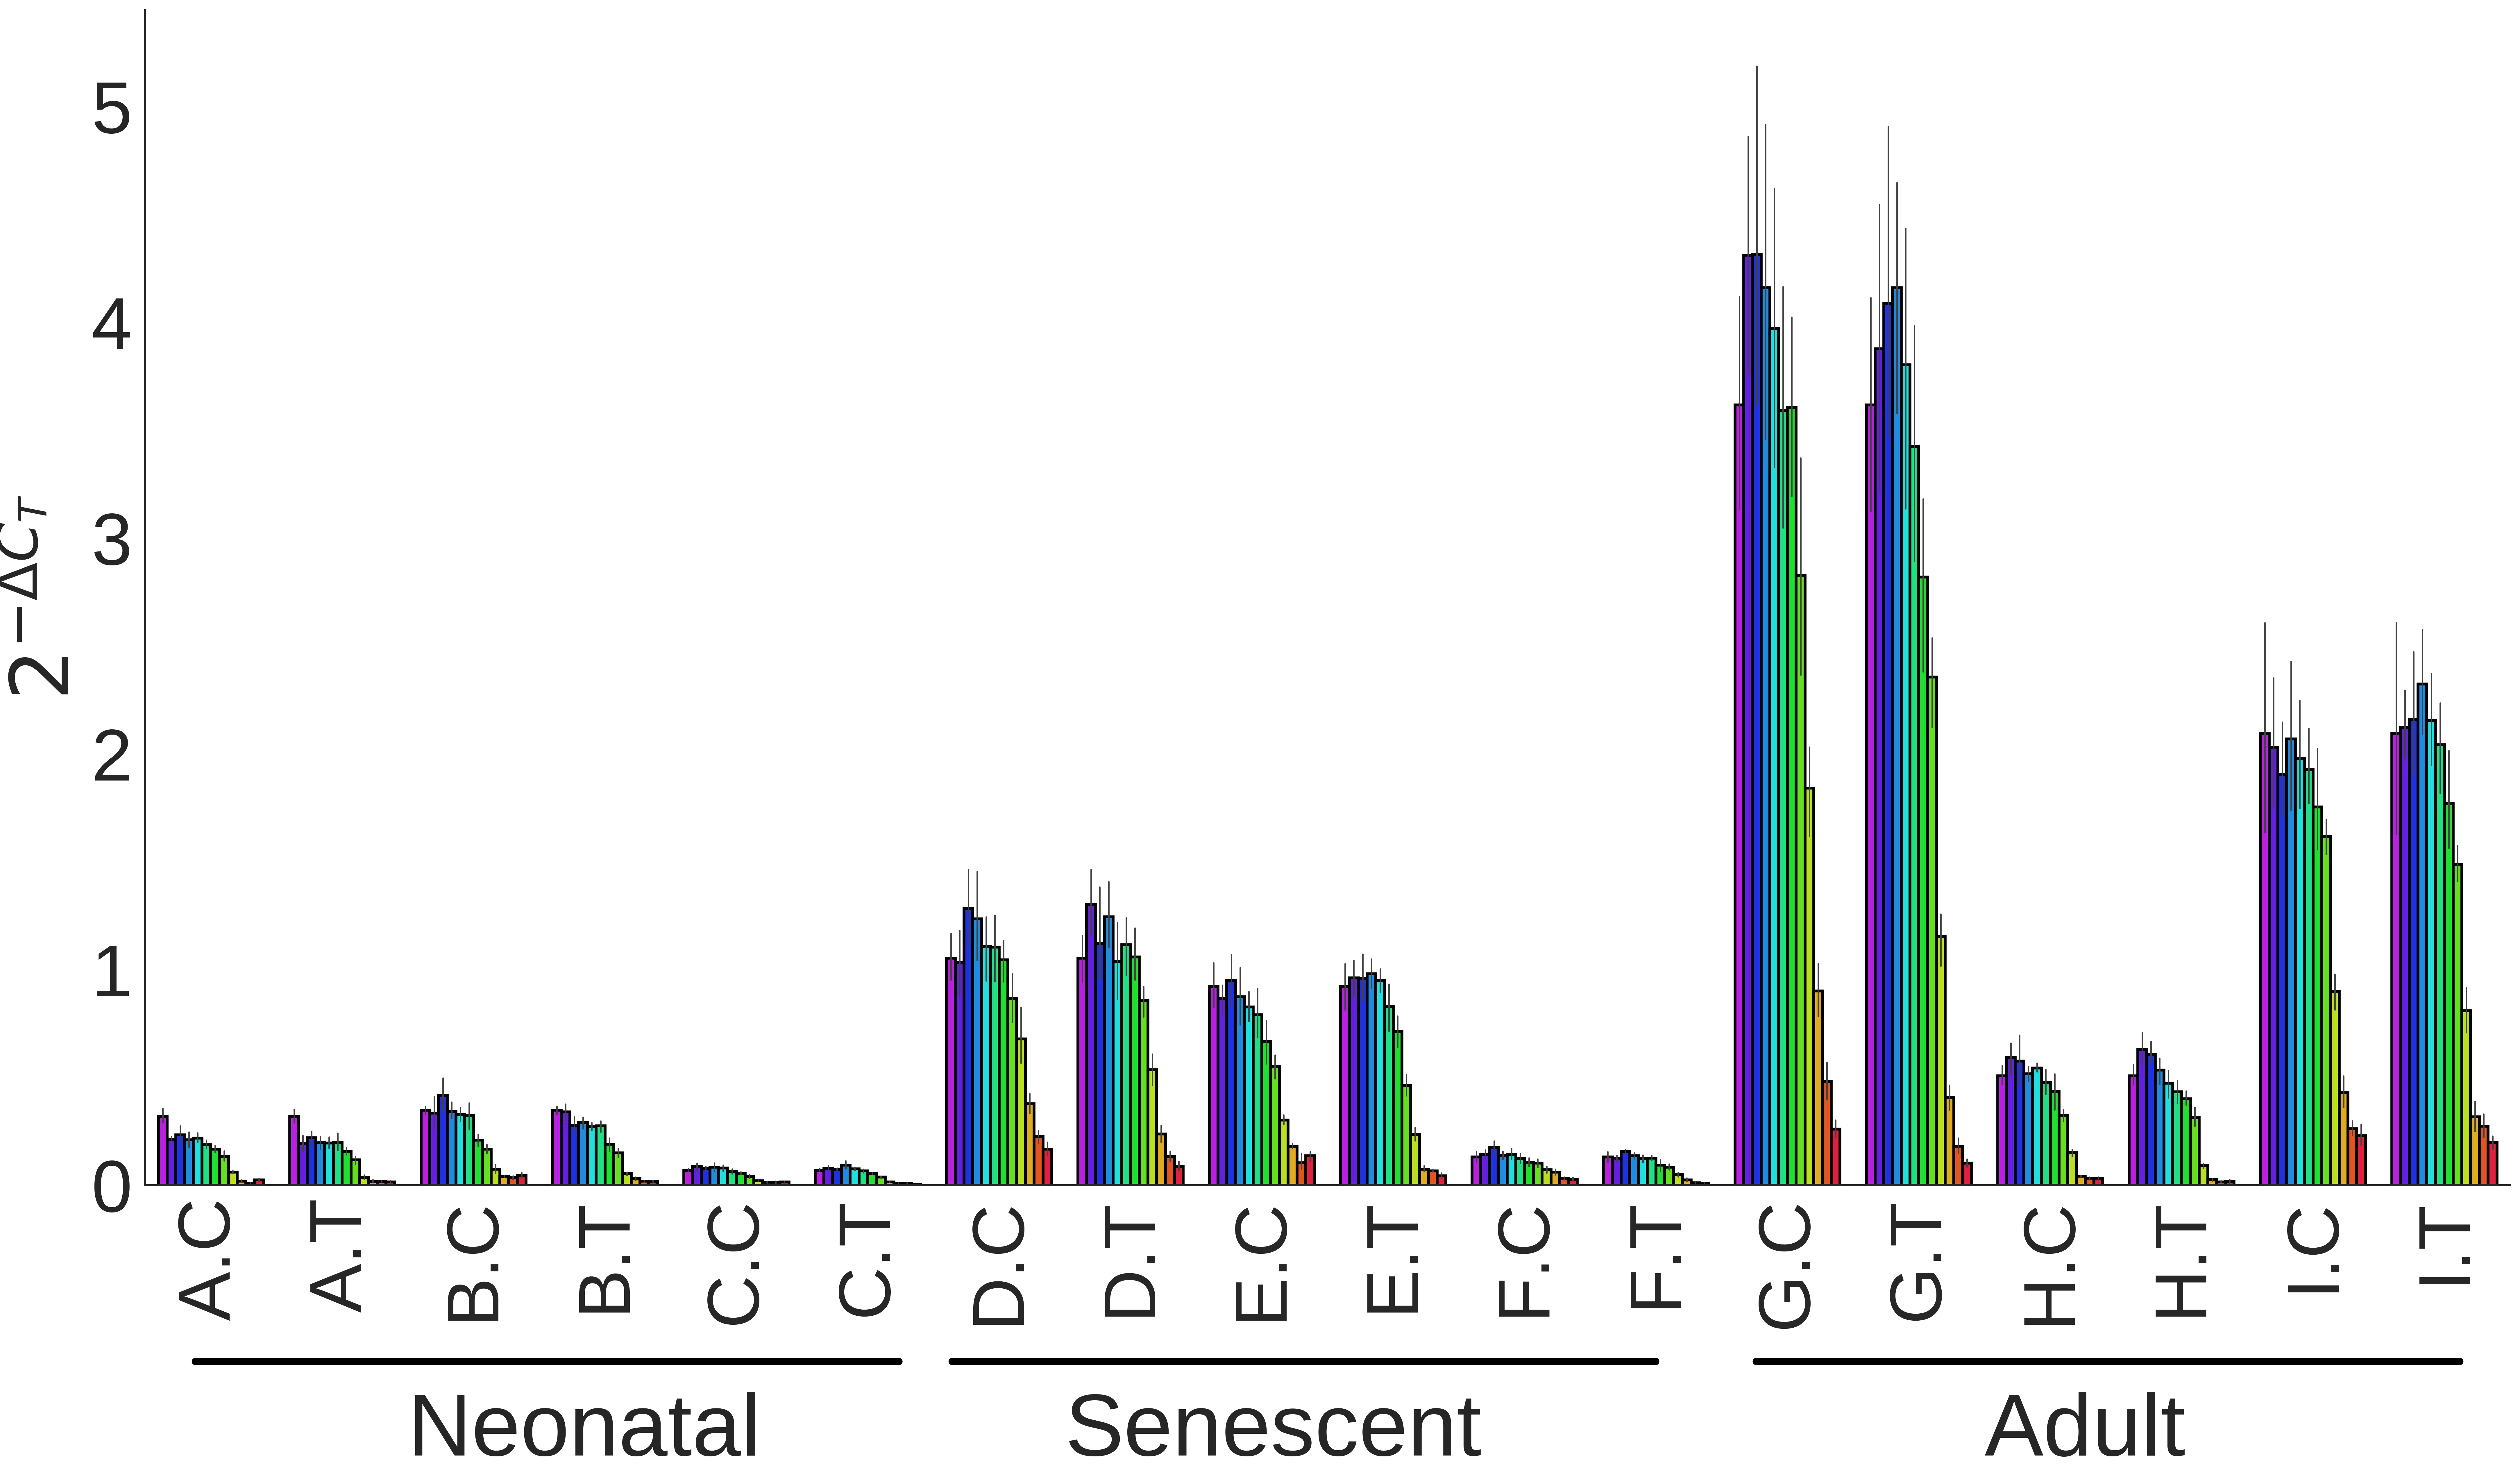
\includegraphics[width=\textwidth]{img/dct_for_publication_no_legend/MMP1}
			\caption{MMP1}\label{MMP1}
		\end{subfigure}\hspace*{\fill}
		\begin{subfigure}[b]{0.45\textwidth}
			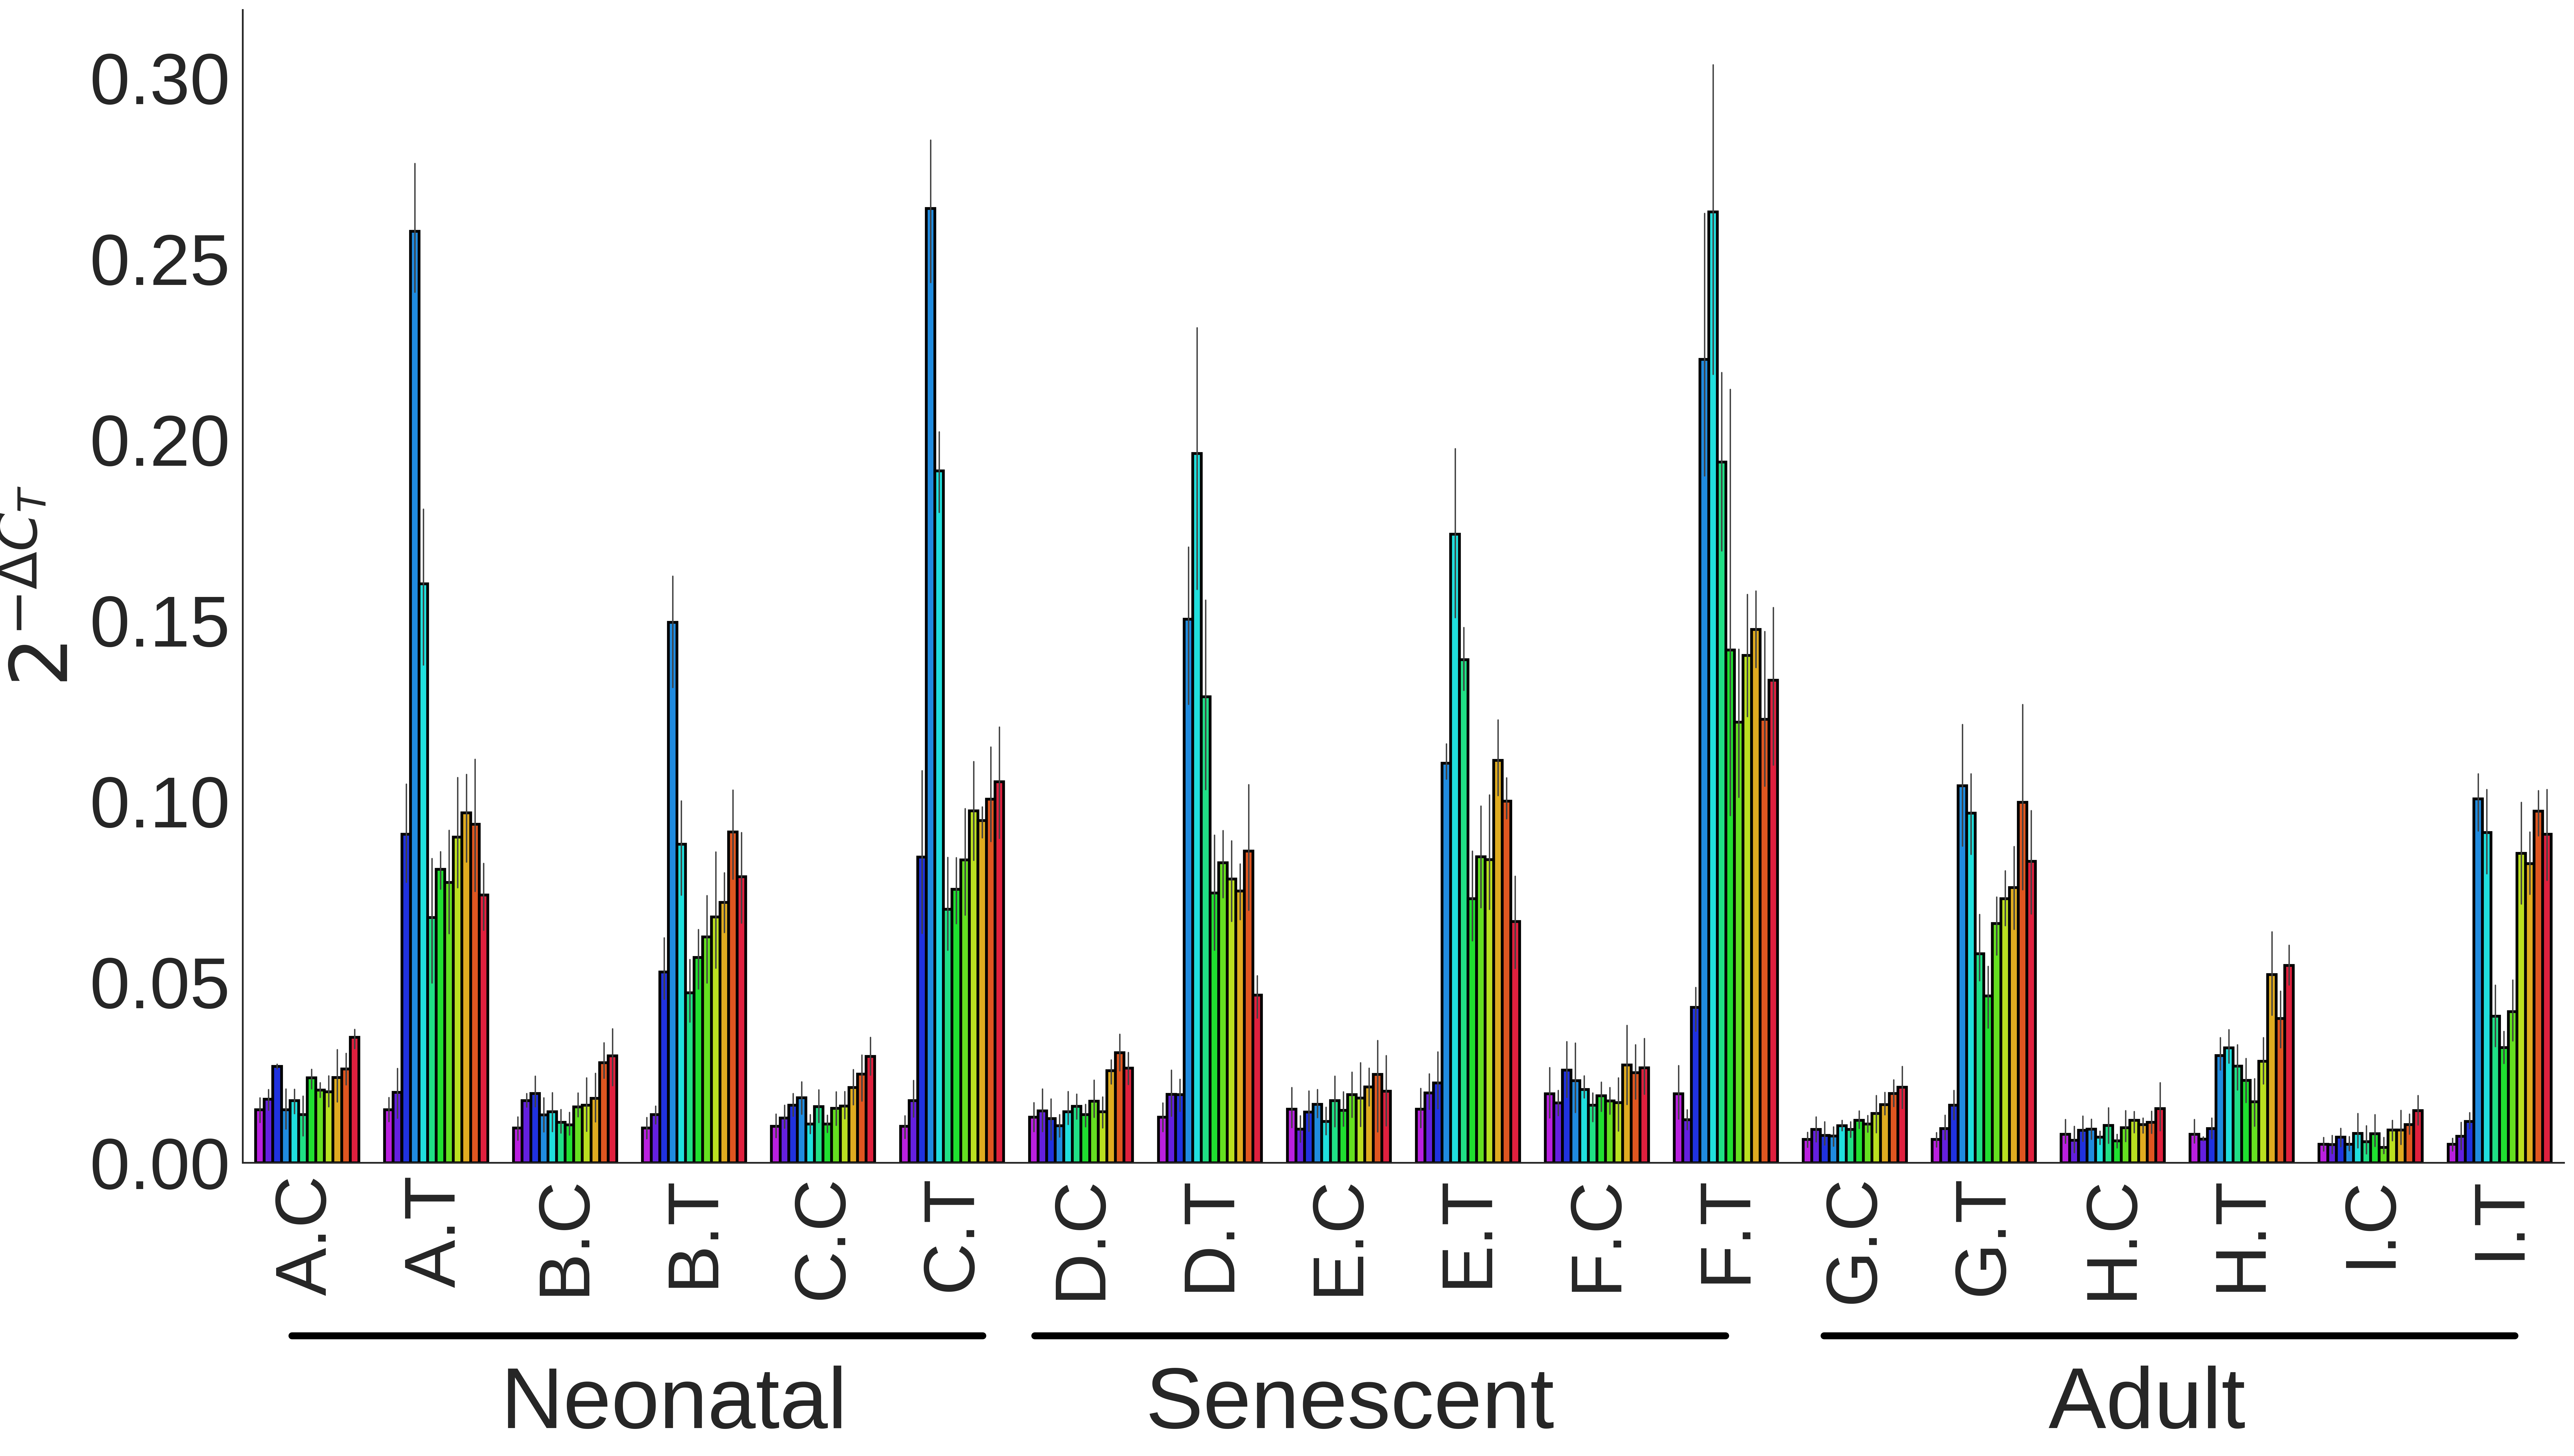
\includegraphics[width=\textwidth]{img/dct_for_publication_no_legend/SMAD7}
			\caption{SMAD7}\label{SMAD7}
		\end{subfigure}\hspace*{\fill}
		
		\begin{subfigure}[b]{0.45\textwidth}
			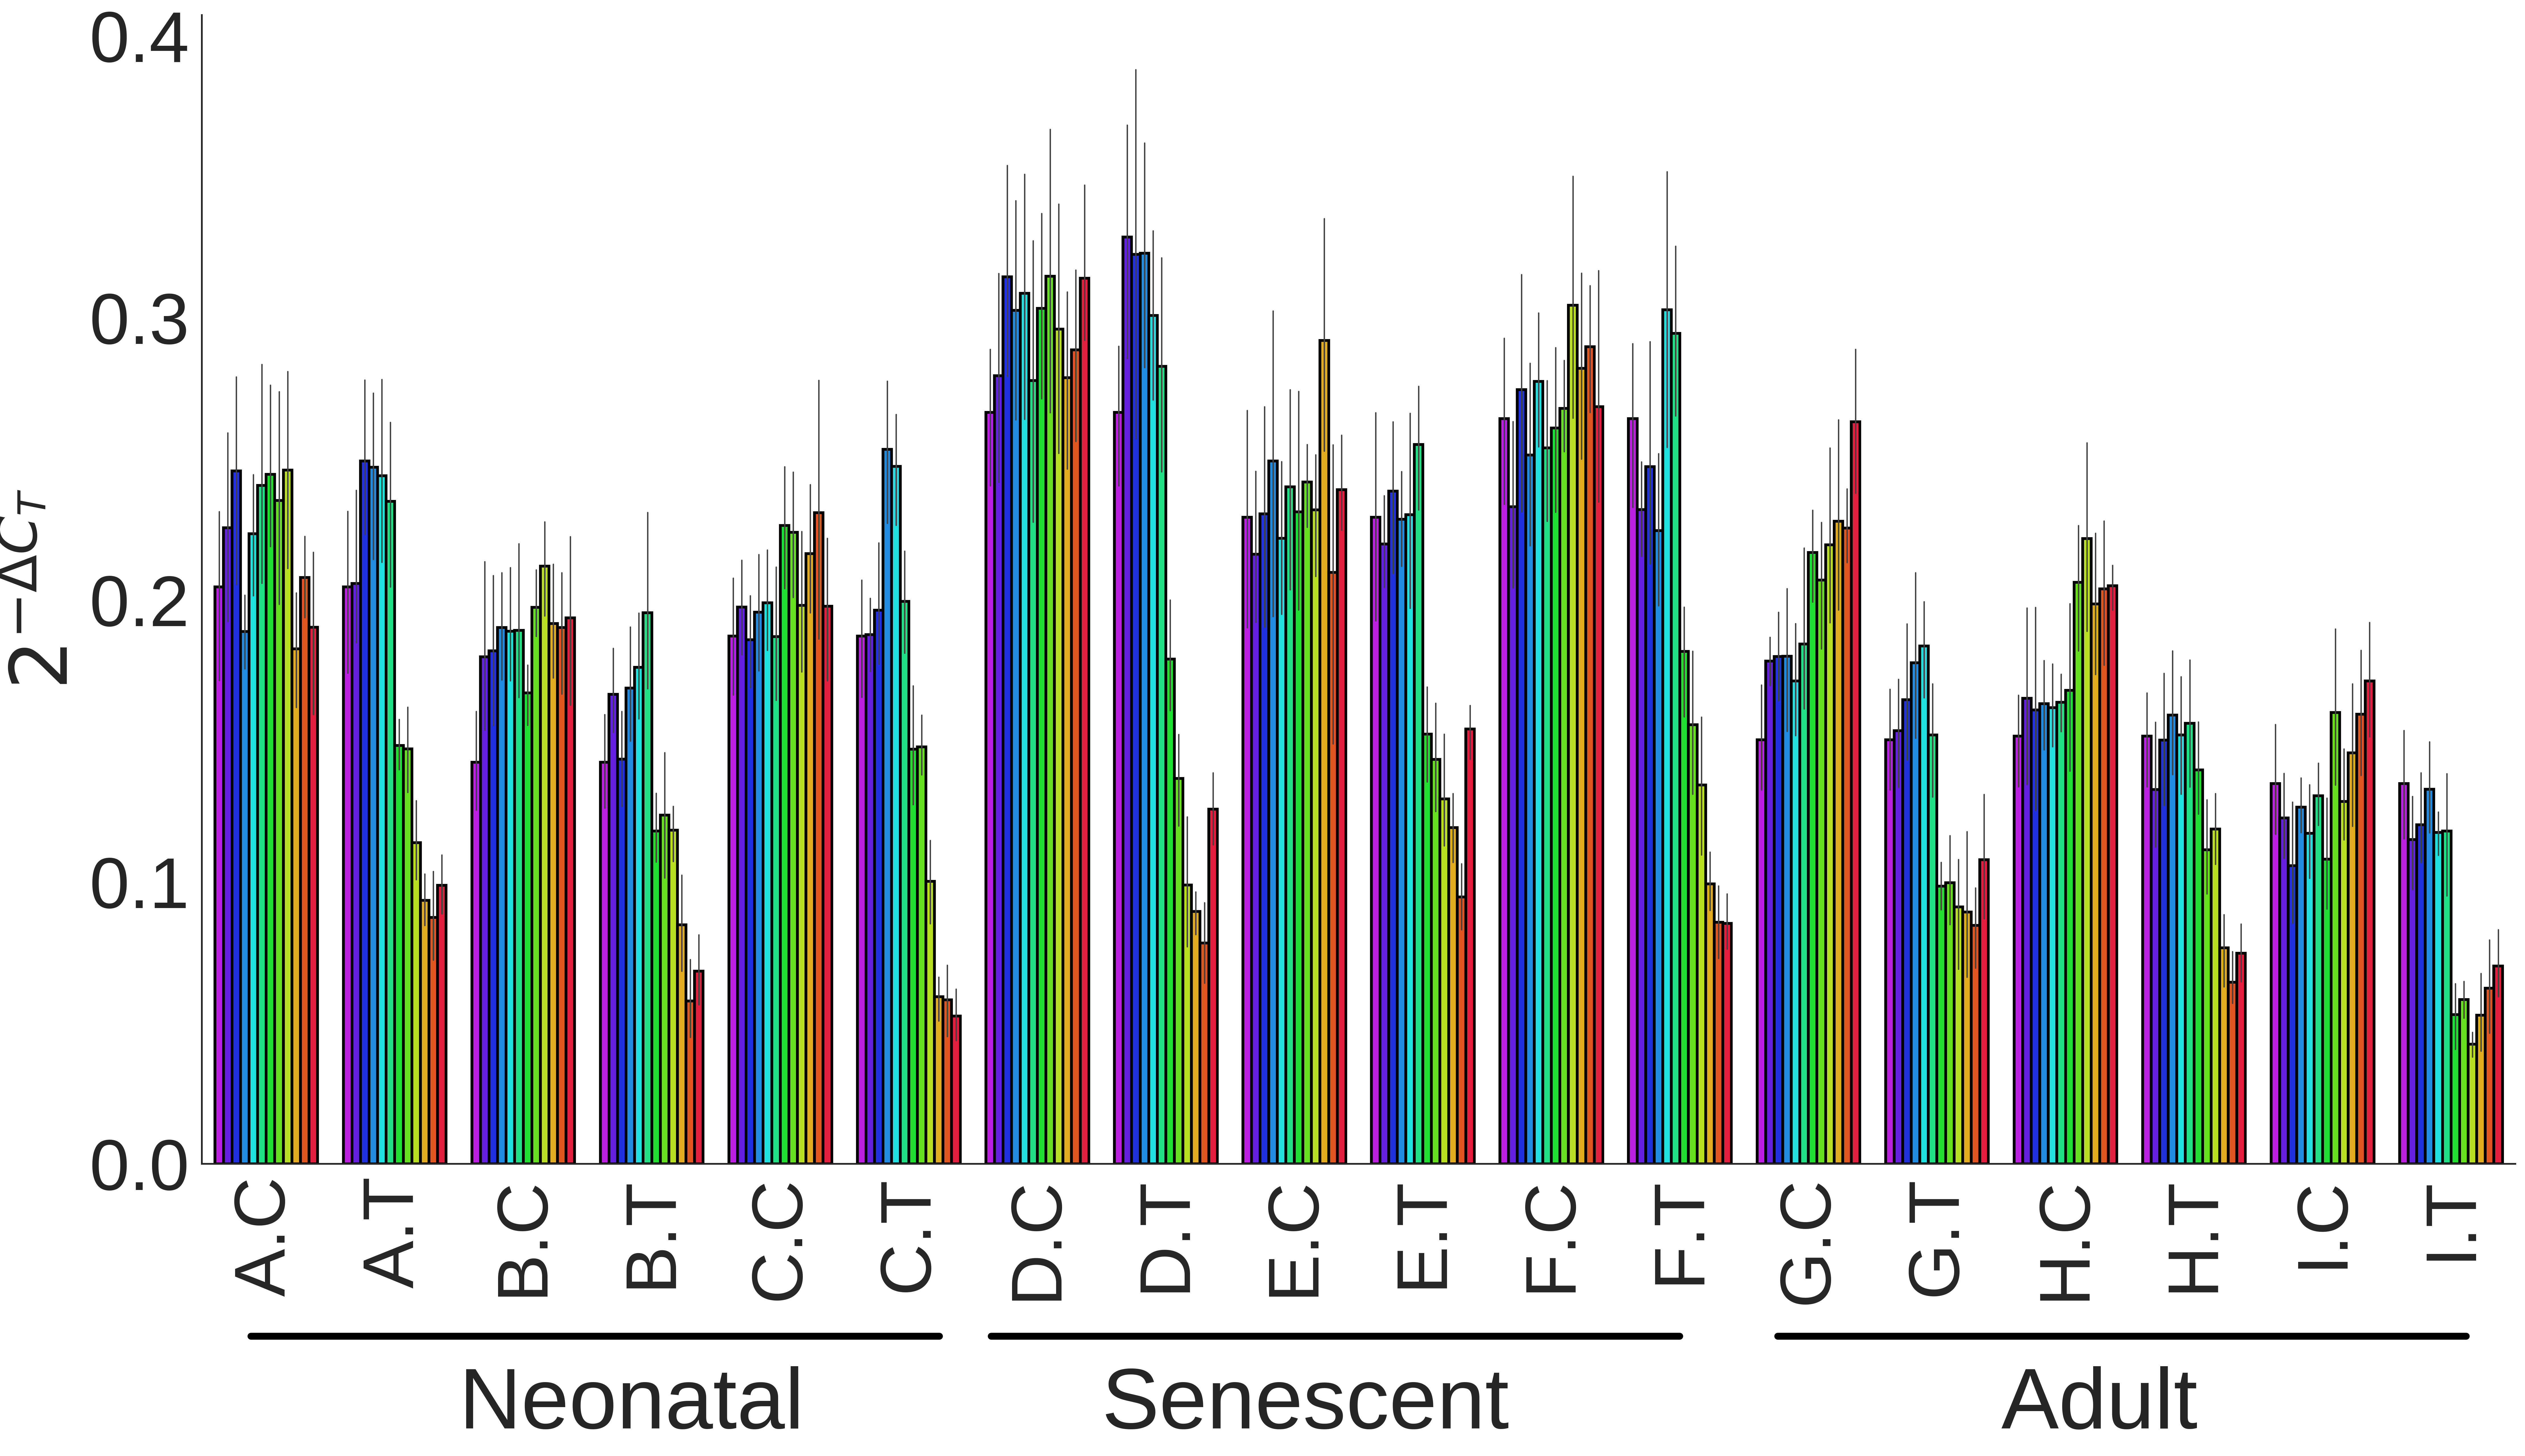
\includegraphics[width=\textwidth]{img/dct_for_publication_no_legend/SMAD3}
			\caption{SMAD3}\label{SMAD3}
		\end{subfigure}\hspace*{\fill}
		\begin{subfigure}[b]{0.45\textwidth}
			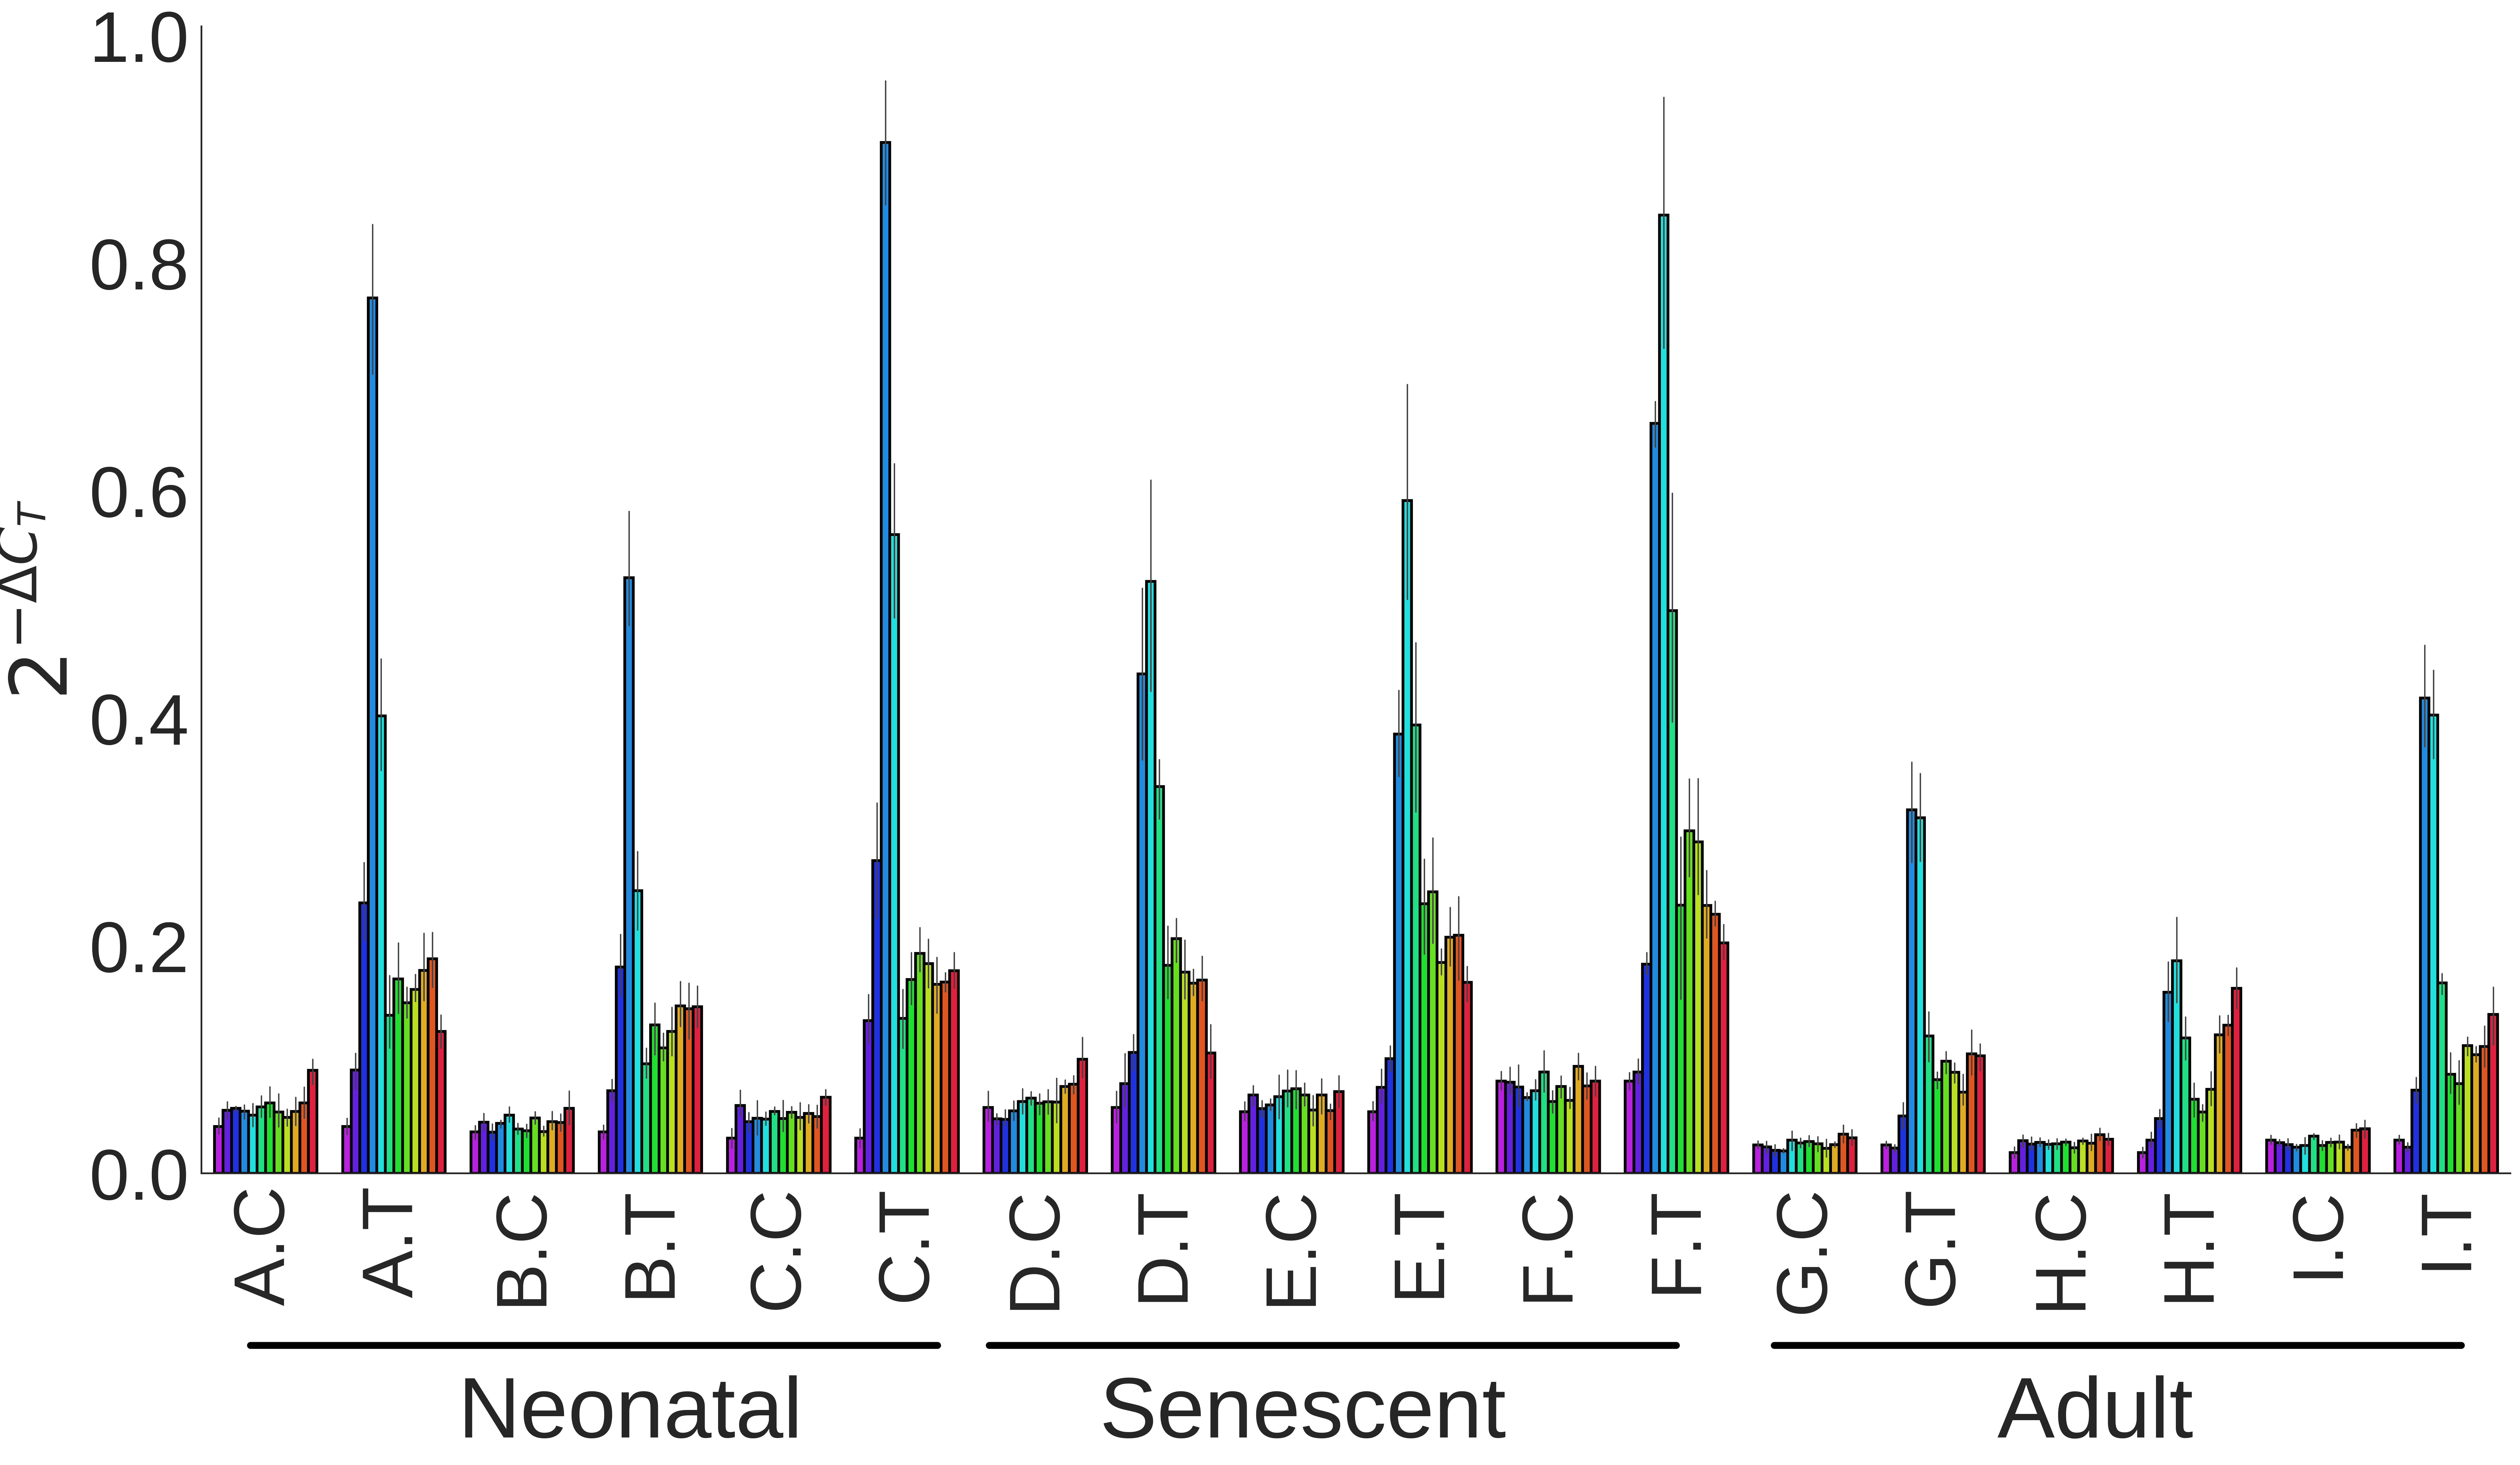
\includegraphics[width=\textwidth]{img/dct_for_publication_no_legend/JUNB}
			\caption{JUNB}\label{JUNB}
		\end{subfigure}\hspace*{\fill}
	\end{minipage}% <--- don't forget
	\begin{minipage}{0.1\textwidth}
		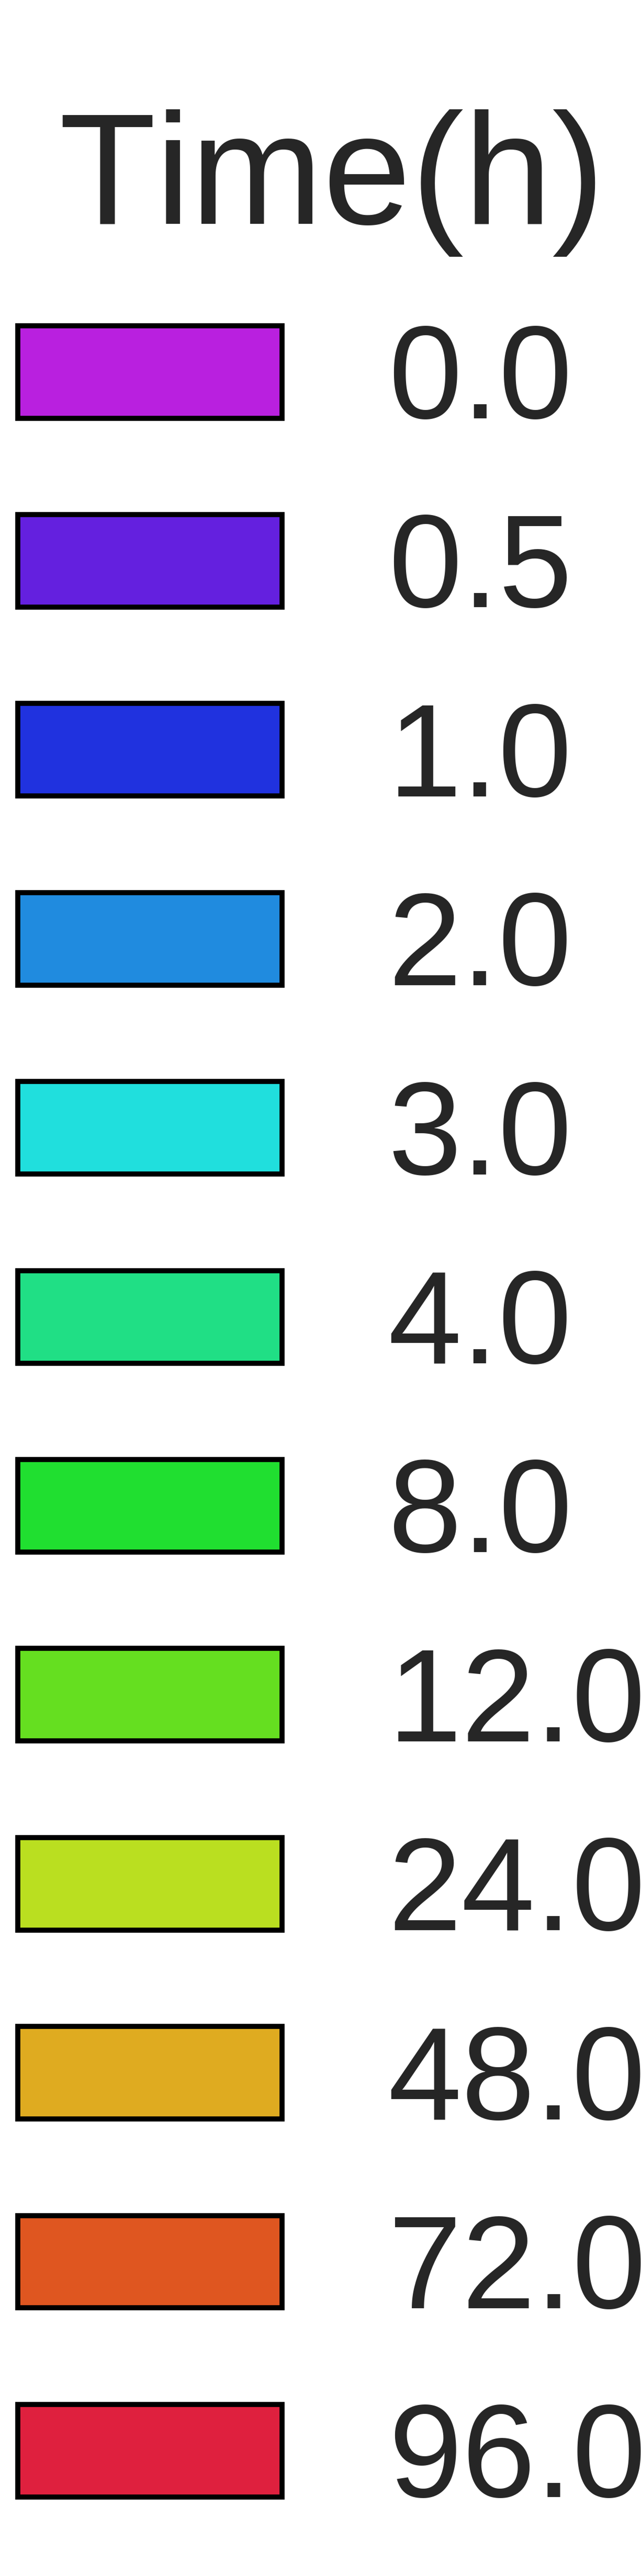
\includegraphics[width=\textwidth,height=8cm]{img/dct_for_publication_no_legend/legend}
	\end{minipage}
	\caption{Bar graphs showing control (C) and \tgf{} (T) treated time series datasets for each cell line (labelled A-I as described in the methods). Error bars represent standard error of the mean and each conditions was repeated 6 times.}
	\label{fig:bar_graphs}
\end{figure}
Since we have data from 3 cell lines per cell line group, we made use of the available data by repeating the LIMMA analysis for all combinations of cell line under a comparison. A total of 10 differential expression analyses were conducted, 5 each to compare \tgf{} or negative control time series, two of which were `between' groups comparisons and three `within' groups comparisons. The output from LIMMA is a list of FDR-corrected p-values representing the probability that two groups are equal. Usually, a p-value threshold is chosen and any gene with a p-value lower than that threshold is considered differentially expressed. Since we have 9 equivalent LIMMA analyses for the `between groups` analysis and 3 for the `within groups' analysis, a consensus strategy was used where if a gene was considered differentially expressed in >60\% of LIMMA analyses, the gene was considered differentially expressed. To investigate the impact of choosing different p-values, the numbers of differentially expressed genes were recorded as a function of p-value and are displayed in \cref{fig:pvalues}. For all p-values, the comparison between adult and neonatal cell lines treated with \tgf{} contained the most differentially expressed genes (\cref{fig:pvalues:between}). Similarly, in all cases the comparison within the adult group treated with \tgf{} contained the second largest group of differentially expressed genes while the comparison within the control neonatal cell lines contained the least (\cref{fig:pvalues:within}). Given that these interpretations are the same for the different p-values, a FDR-adjusted p-value of 0.001 was considered a reasonable balance between too strict and too lenient. A detailed summary of the differential expression analysis is presented in \cref{fig:heatmap} using a p-value threshold of 0.001 while the number of genes that were differentially expressed in >60\% of LIMMA analyses were counted and displayed in \cref{table:stats_summary}.

\subsection{Dynamic gene expression profiles}
So far we have gained a broad overview of the data using PCA and a detailed view of the statistics drawn from the data using a differential expression analysis in LIMMA. In this section we have selected 8 genes for a more detailed discussion (\cref{fig:bar_graphs}). However, the full, A4 sized dataset is available for download in supplementary file 1. As an alternative, the data that we present here are available for exploration and download at \url{http://cwelsh2.pythonanywhere.com/}. 

Collagen 1A1 and 1A2 are the first two of the 8 genes chosen for discussion (\cref{COL1A1, COL1A2}). Both genes were strongly induced by \tgf{} but were also produced in the control condition. Comparing adult and neonatal cell lines, it is clear than the adult cell lines produce less COL1A1 and COL1A2 than neonatal cell lines. 

ACTA2 ($\upalpha$-SMA) and CTGF were both chosen for discussion because they are among the most strongly induced of the genes measured. \tgf{} strongly induced both ACTA2 \cref{ACTA2} and CTGF \cref{CTGF} in all cell lines and like the collagen profiles, the induction was considerably weaker in adult cell lines. 

MMP1 production diminished over time in all 9 cell lines and in both the control and \tgf{} treated samples \cref{MMP1}. This indicates that the observed decline in MMP1 mRNA over time was not a result of \tgf{} treatment. Both senescent and adult cell lines produced more MMP1 than the neonatal cell lines and the adult cell lines produced more MMP1 than the senescent cell lines. However there is a degree of heterogeneity regarding the MMP1 profile, given that in all cell lines groups, one out of three cell lines produced considerably less MMP1 than the others. 

Smad7, Smad3 and JunB are all signalling components of the \tgf{} network. Smad7 was present in small quantities in the control cell lines and \tgf{} treatment quickly and transiently induced Smad7 transcription in all cell lines (\cref{SMAD7}). The peak magnitude was similar between senescent and neonatal cell lines but blunted in adult cell lines. Smad3 was similarly unaffected by the control treatment but a reduction in the amount of Smad3 mRNA declined between 8h and 24h after \tgf{} stimulation (\cref{SMAD3}). The dynamics of the JunB profile are similar to Smad7, with a transient spike occurring 2h post \tgf{} stimulation, but not in the control time series (\cref{JUNB}). The amount of \tgf{} induced JunB is diminished in adult compared to neonatal cell lines. 

\section{Discussion}
In aged skin, the composition of the dermal ECM changes resulting in thinner, weaker and less elastic skin \citep{Farage2009}. While it is known that the composition of an aged dermis is differs from young tissue, much is still unknown regarding how they differ. To gain a better understanding of what differences exist between young and old skin, we conducted a high throughput qPCR experiment to measure the activity of 72 genes over time in neonatal, adult and irradiation-induced senescent fibroblasts. Since \tgf{} is a key mediator positively regulating ECM homeostasis \citep{Hinz2015}, we treated fibroblasts with \tgf{} and a negative control to observe how the different cell lines respond. 

The PCA and the differential expression analysis conducted in this study represent two different means of extracting information from this dataset. The PCA provides a broad overview of the data and clearly shows the response to \tgf{} is considerably different between cell line groups (\cref{fig:qc:cell_line}). The differential expression analysis on the other hand, provides a detailed indication of which genes are different between groups. A notable observation is that in all comparisons between and within cell lines, the \tgf{} treated time series always contained more differentially expressed genes than the control group. This finding may ... <note for daryl: what is the interpretation here? Is this result to be expected. Is it biologically significant?>. 

The comparison between the \tgf{} treated adult and neonatal cell lines had the most differentially expressed genes (\cref{fig:between:heatmap,fig:pvalues:between}). This provides strong support for the contention that old fibroblasts behave differently from young. The comparison within the \tgf{} treated adult cell line group was the second largest number of differentially expressed genes, while the comparison within the control treated neonatal cell lines had the least numbers of differentially expressed genes (\cref{fig:within:heatmap,fig:pvalues:within}). These two findings are intuitive results because it is known that heterogeneity increases with age (\cite{Watt2011}). 

In \cref{fig:bar_graphs}, we have selected a subset of the measured genes for discussion. Our measurements for type 1 collagen agree with previous reports that type 1 collagen is reduced with age. \cite{Varani2006} found that type 1 procollagen levels were 3 times lower in aged (80+) compared to young (18-29) individuals (15ng/mm$^2$ compared to 5ng/mm$^2$ respectively). Moreover, data presented in \cite{Quan2010} agrees with this assessment. \cref{COL1A1, COL1A2} shows that our data agree with these reports that \tgf{} strongly induces the production of collagen from fibroblasts and that the amount produced is reduced in age. It is interesting to note that the amount of COL1A1 produced is approximately double that of COL1A2, in line with the knowledge that the stoichiometry for type 1 collagen heterotrimers two COL1A1 to one COL1A2 chain (ref). 

\tgf{} induces proliferation of fibroblasts and their differentiation to myofibroblasts \citep{Liu2016, Negmadjanov2015}. Normally fibroblasts are in a quiescent state, controlling the normal homeostasis of dermal tissues. Under physiological responses such as wound repair, fibroblasts undergo differentiation and change their phenotype to an `active' myofibroblast state which display characteristics of smooth muscle cells. \sma{} is a marker for myofibroblasts \citep{Zanotti2010, Evans2003} which facilitates contraction of a wound \citep{Darby2007}. \cref{ACTA2} therefore indicates that \tgf{} induces differentiation of fibroblasts to myofibroblasts. Assuming \sma{} is an accurate marker for myofibroblasts, \cref{ACTA2} shows that adult fibroblasts ability to differentiate is severely impaired compared to neonatal and damage-induced senescent fibroblasts. This implies that when older cells needs to produce large quantities of ECM they are unable to do so with the same vigour as young cells. Therefore, lack of differentiability may mechanistically be related to why wound healing takes longer in the elderly. 

CTGF is an important regulator of fibrotic signalling pathways and is a downstream target of \tgf{} (\cite{Quan2002, Wahab2005, Ponticos2009}). Evidence that blocking CTGF signalling reduces the amount of collagen produced by sclerotic fibroblasts emphasises the relationship between CTGF and collagen levels \citep{Makino2017, Sonnylal2010}. Our data agrees with previous reports that \tgf{} strongly induces CTGF expression in fibroblasts \cref{CTGF}. Moreover, our data agrees with \citep{Quan2010} in that CTGF production is diminished in older fibroblasts.

Reduced collagen levels with age may result from both reduced production and increased degradation. MMPs are proteases in the extracellular matrix, some of which, including MMP1, can degrade collagen. It has been shown that the aged dermis produces higher levels of MMPs compared to younger individuals (ref). Specifically, \citep{Qin2017} showed that the aged dermis contained higher levels of MMP1, MMP3, MMP9, MMP10, MMP11, MMP23, MMP24, MMP27 and MMP28 compared to young dermis. In agreement with \cite{Qin2017}, our data suggest that \cref{MMP1} MMP1 expression is enhanced in aged tissue compared to young and that a degree of heterogeneity exists regarding MMP1 levels in age. 

The MMP1 response to \tgf{} (\cref{MMP1}) is a surprising result that distinguishes this experiment from other reported studies. \cite{White2000} characterised a \tgf{} inhibitory element (TIE) in the MMP1 promoter that is involved in constitutive MMP1 repression. Further, both \cite{White2000} and \cite{Edwards1996} observed that \tgf{} inhibited PMA-induced MMP1 production, while \citep{Yuan2001} observed that \tgf{} inhibited IL-1$\beta$ production. These data point towards \tgf{} mediated transcriptional repression of MMP1, which is an attractive idea because it is intuitive from a resource allocation point of view that if \tgf{} directs anabolic processes, than catabolic processes should be inhibited. However, contrary to this hypothesis, MMP1 did not positively or negatively respond to \tgf{} stimulation in any of the age or senescent cell lines and this result robust across all 9 cell lines under study (\cref{MMP1}). A hypothesis to explain this apparent discrepancy is that in \citep{White2000, Edwards1996, Yuan2001}, \tgf{} only inhibited an increase in MMP1 production that was induced by either TPA or IL-1$\beta$. On the other hand, we have measured the MMP1 response to \tgf{} or a negative control, without prior stimulation with a positive regulator of MMP1. Thus a plausible conclusion consistent with all the evidence is that \tgf{} inhibits induced-MMP1 synthesis, but not basal MMP1 production. The time matched controls were pivotal in reaching this conclusion because if only a 0 time point control was used then it would appear as though \tgf{} induced a reduction in MMP1 transcription. The data in \cref{MMP1} emphasises the importance of time matched controls when studying the dynamics of biological systems.
%%% \citep{Fisher2009} Found MMP1 up in age. Incorporate. 

%While Smad3 is the most important effector Smad for ECM regulation \citep{Li2003}, 
Smad7 is the most important negative feedback of the Smad system \citep{Hayashi1997, Nakao1997, Yan2016, Gersdorff2000, Ebisawa2001, Hanyu2001, Pulaski2001, Suzuki2002, Shi2004, Zhang2007}. Smad7 both negatively regulates Smad signalling and represents a mechanism of cross-talk with other signalling pathways (\cite{Yan2011}). A considerable portion of the work that studied Smad7 has been conducted on keratinocyte (HaCaT) cell lines and indicate that Smad7 levels peak at approximately 1h post-\tgf{} stimulation (\cite{Denissova2000}). \cref{SMAD7} provides evidence that in fibroblasts, Smad7 mRNA levels peaks between 1 and 3h post-\tgf{} stimulation. In neonatal and senescent cell lines, a second peak in Smad7 production was observed 48-72h post-\tgf{} stimulation. In adult cell lines the magnitude of the first peak is markedly reduced compared to neonatal cell lines. It is not clear what the biological purpose of this second peak in Smad7 production is but given that Smad7 inhibits the Smad signalling pathway, its likely that canonical Smad signalling is not active at these later time points. It is also unclear what the biological implications of reduced Smad7 production in age has on the \tgf{} biology. It may be that Smad7 production is lower in adult cells because Smad signalling is impaired and requires less inhibition. 

Smad3 is a prototypical effector of \tgf{} signalling and essential for the transcription of type 1 collagens \cite{Runyan2003}. \cite{Purohit2016} observed reduced Smad3 levels in both age and senescent fibroblasts and showed using silencing RNA experiments that reduced Smad3 could account for the observed reduction in type I procollagen in the aged dermis. While it is certainly feasible that less Smad3 in adult cells would cause reduced collagen production, \cref{SMAD3} only provides weak support for this hypothesis since the differences between adult and neonatal cell lines are not so profound. However, just because this data does not provide good support for a transcriptional mechanism of Smad3 decline in age does not preclude the possibility that Smad3 protein levels are reduced in age because of an alternative mechanism, such as enhanced Smad3 degradation. Therefore the role of Smad3 in ageing fibroblasts is still an open question, but based on this data it is unlikely to involve a transcriptional mechanism. 

An interesting aspect of the Smad3 data is that 8-12h post stimulation by \tgf{}, Smad3 mRNA levels are reduced to what appears to be a new steady state (\cref{SMAD3}). This observation suggests the existence of a late acting negative feedback in the \tgf{} response to persistent \tgf{} stimulation. To our knowledge, this insight into Smad signalling is novel. It is noteworthy that the timing of the drop in Smad3 mRNA levels directly precedes the incline in \sma{} and so a hypothesis is that this drop in Smad3 mRNA occurs before or during fibroblast differentiation, though this would need experimental testing. 

A limitation of this study is that we have measured only 72 genes. While it would have been more informative to measure all activity of all genes instead (for example by microarray or RNA-seq), the use of high throughput qPCR enabled the measurement of more experimental conditions. In turn, we were able to design our experiments as time series to measure the dynamics of gene expression over time. Despite choosing the 72 genes to be as relevant to the subject of skin ageing as possible, there are inevitably others which we have not been able to measure, and so our analysis is based on a bias selection of genes. 

Biological function operates at the protein level of biological organisation, but we have only measured mRNA. While still valuable, since there is not necessarily a one-to-one correspondence between mRNA and protein \citep{Liu2016}, it would be illuminating to perform some parallel proteomic and phosphoproteomic experiments to provide a more comprehensive understanding of the differences between young and old fibroblast behaviour.

Another limitation of this work is that irradiation-induced senescence was used as a model for replicative senescence. It has been shown that there strong similarities between the replicative and irradiation-induced senescence \citep{Marthandan2016}, but there still may be important differences which should be considered when drawing conclusions about replicative senescence from a irradiation-induced senescence model. 

In this work we have studied the dynamic response of three groups of cells: neonatal, adult and irradiation-induced senescent fibroblasts. We have shown that considerable differences exist between the response of these three cell types both in response to \tgf{} and without stimulation. We have discussed a selection of the data and have built an interface which is available for interactively exploring both the time series and the PCA data. We envision that the data presented here combined with some protein level data will be useful for incorporation into mechanistic models that describing the differences in signal transduction biochemistry between young and old fibroblasts.

\section{Materials and methods}
\subsection{Cell Culture}
Three independent human neonatal dermal fibroblasts (HDFn) labelled A (Caucasian male, catalogue number: C-004-5C, lot number: \#1366434 ), B (Caucasian male, catalogue number: C-004-5C, lot number: \#1366356) and C (Caucasian male, catalogue number: C-004-5C, lot number: \#1206197); three irradiation-induced senescent cell lines (D, E and, F) which are the same as A, B and C respectively but irradiated with 20Gy ten days prior to seeding, and three adult cell lines G (55 years old Caucasian female, catalogue number: C-013-5C, lot number: \#1528526), H (60 year old, Caucasian male, catalogue number: A11634, lot number: \#1090465) and I (65 year old, Caucasian female, catalogue number: A11636, lot number: \#200910-901) were purchased from Life Technologies and seeded into standard tissue culture treated 12-well dishes at a density of 10,000 cells/cm$^2$ in 3.5ml M106 medium (ThermoFisher Scientific, catalogue number: M106500) supplemented with LSSG (ThermoFisher Scientific, catalogue number: S00310) and at 27$^{\circ}$C, 5\%CO$_2$ for 4 days. Senescent cells were seeded at higher density of 65,000 cells/cm$^2$.
%
\subsection{Treatment Protocol}
Cells from each cell line were serum starved 24h prior to treatment by removing LSGS supplementation from media. Following 24h of incubation at 37$^{\circ}$C and 5\% CO$_2$, cells were assigned one of three treatments: baseline, control or \tgf{}. Baseline samples were not treated in any way prior to harvesting at experiment start (0h) and end (96h). \tgf{} and control samples were treated with media containing 5ng mL$^{-1}$ \tgf{} reconstituted in 10mM citric acid or 0.1\% BSA in 10mM citric acid respectively. In control and \tgf{} groups, cells were harvested at 0.5, 1, 2, 3, 4, 8, 12, 24, 48, 72, 96 hours post treatment. All 216 conditions were repeated 6 times resulting in 1296 individual samples. Samples were shipped to Procter and Gamble (P\&G), Cincinnati for quantification on a high throughput PCR Smart chip platform by WaferGen.

\subsection{High throughput qPCR smart chip}
-include the randomisation procedure used on the plates. 

\subsection{Normalization}
The raw data (containing cycle threshold values) is available for download in supplementary file 2. Each gene measured in each sample was normalised to PPIA, the gene which encodes for peptidylprolyl isomerase A which is stationary throughout treatment with \tgf{}. \cref{eq:dct} was used to normalise every gene $g$ of every sample prior to visualisation and differential expression calculations. 
\begin{equation}
\Delta CT_g = 2^{-CT_g - CT_{PPIA}} 
\label{eq:dct}
\end{equation}
The normalised data is available for download from the associated website that hosts the data visualisation application.

\subsection{Differential Expression}
The R package, LIMMA \citep{Smyth2004,Smyth2005, Ritchie2015}, was used to compute differential expression statistics. LIMMA was configured to using a spline matrix with 4 degrees of freedom, as per the LIMMA user guide, to compare either the control time series between adult/senescent and neonatal cell lines or the \tgf{} treated cells. To make use of the available cell line replicates, differential expression calculation was repeated so that all adult/senescent cell lines were compared with all neonatal cell lines. The results were aggregated by calculating the percentage of times a gene has a false discovery rate (FDR) corrected p-value smaller than 0.05. This was repeated for both control and \tgf{} data sets and for both adult and senescent cell lines, compared with neonatal. The R script used is available for download in supplementary file 3.  

\subsection{Website Development}
The website was developed using the Django (version 2.0.5) web framework using Python 3.6. Plotting was conducted using Bokeh and Plotly, which are both Python visualisation libraries. The source code used to build the website is available at \url{https://github.com/CiaranWelsh/data_viz_with_django}. 

\section*{acknowledgements}
Acknowledgements should include contributions from anyone who does not meet the criteria for authorship (for example, to recognize contributions from people who provided technical help, collation of data, writing assistance, acquisition of funding, or a department chairperson who provided general support), as well as any funding or other support information.

\section*{conflict of interest}
You may be asked to provide a conflict of interest statement during the submission process. Please check the journal's author guidelines for details on what to include in this section. Please ensure you liaise with all co-authors to confirm agreement with the final statement.

\printendnotes

\bibliography{references}

\section{Supplementary Figures}
\subsection{Principle Component Analysis}

\begin{figure}[b]
	\centering
	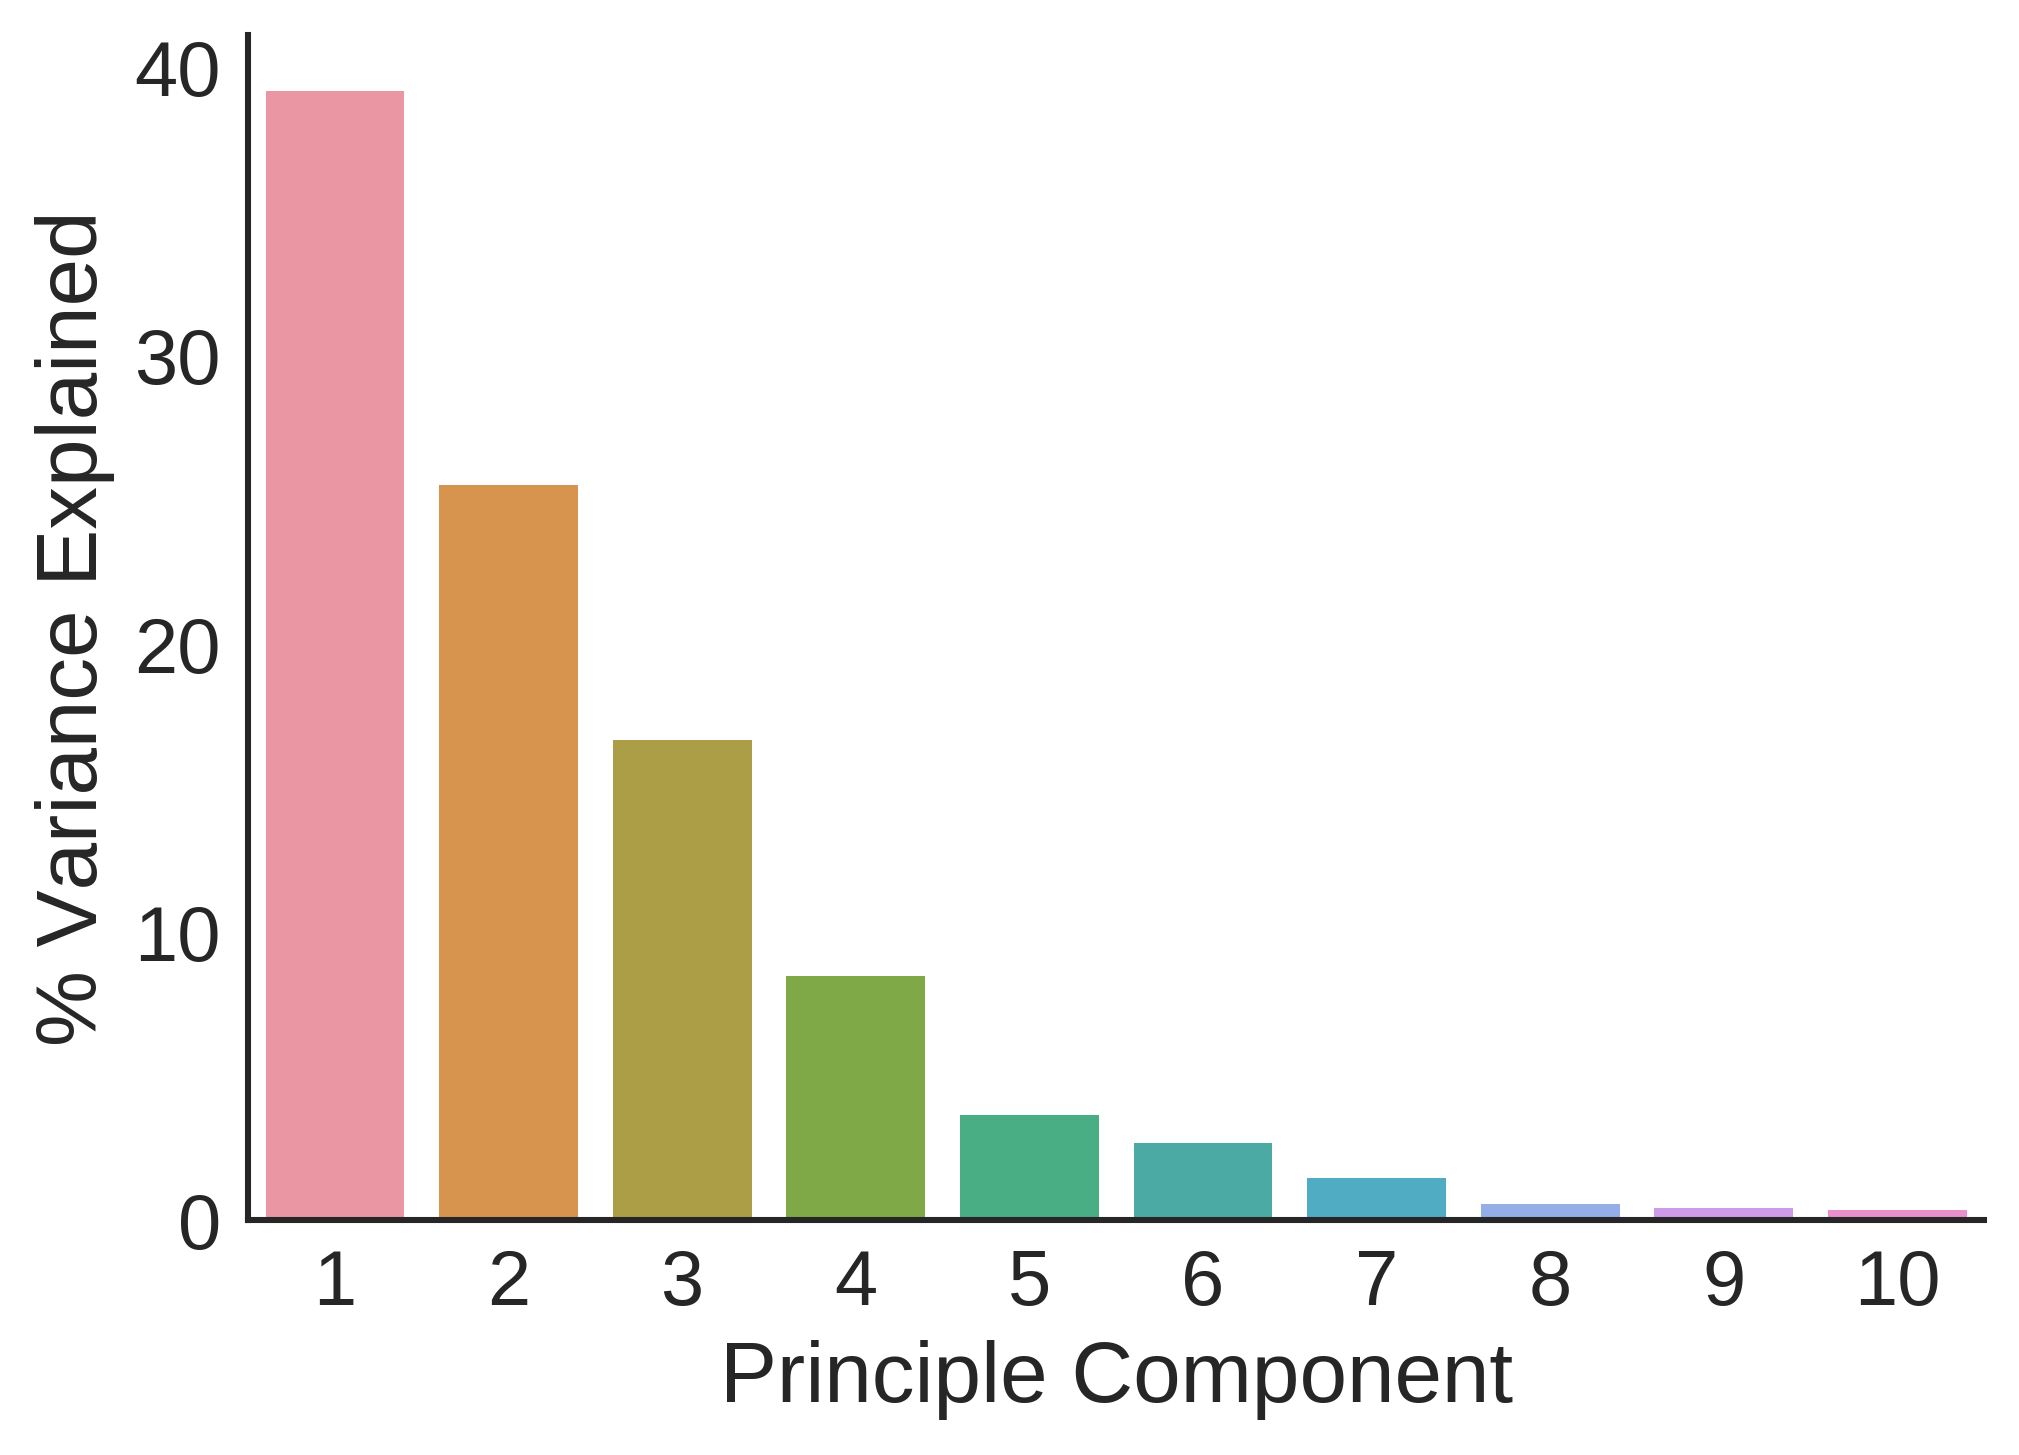
\includegraphics[height=0.35\textheight]{img/qc/pca_scree}
	\caption{Plot showing the percent of variance explained for the first 10 principal components.}
	\label{fig:qc:scree}
\end{figure}

\begin{figure}
	\centering
	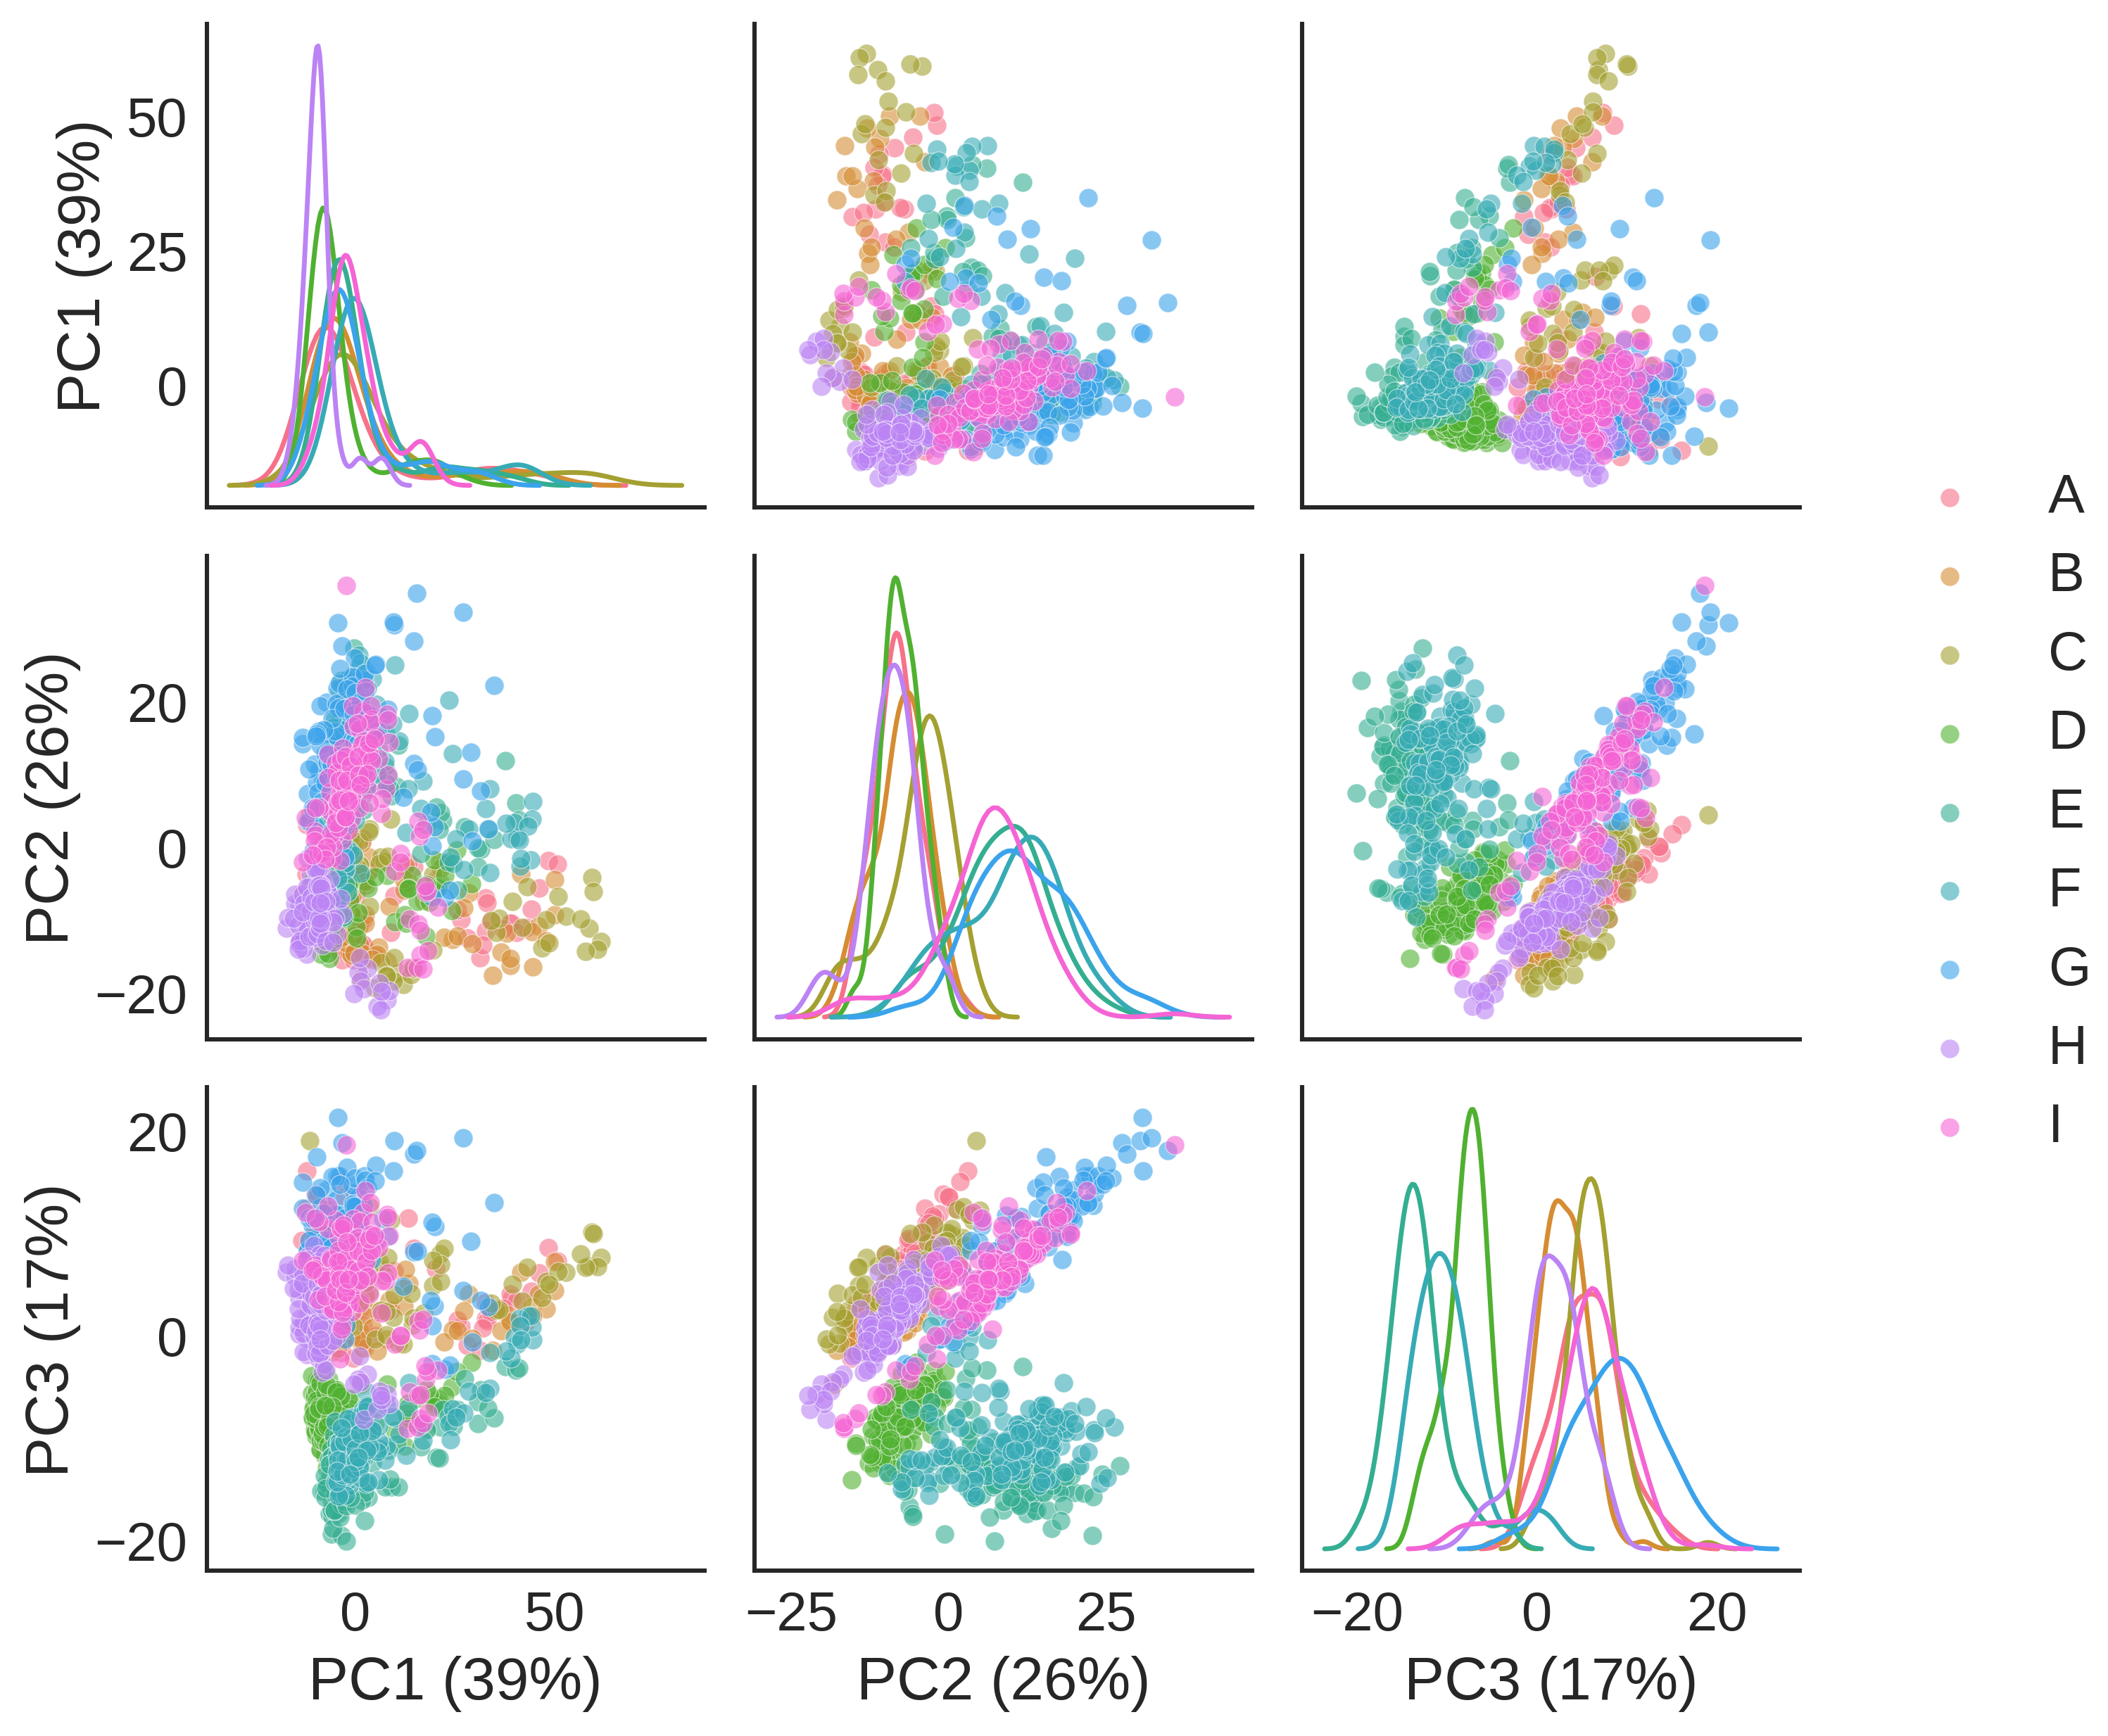
\includegraphics[height=0.45\textheight]{img/qc/cell_id}
	\caption{Scatter matrix of first three principle components coloured by cell id.}
	\label{fig:qc:cell_id}
\end{figure}

\begin{figure}
	\centering
	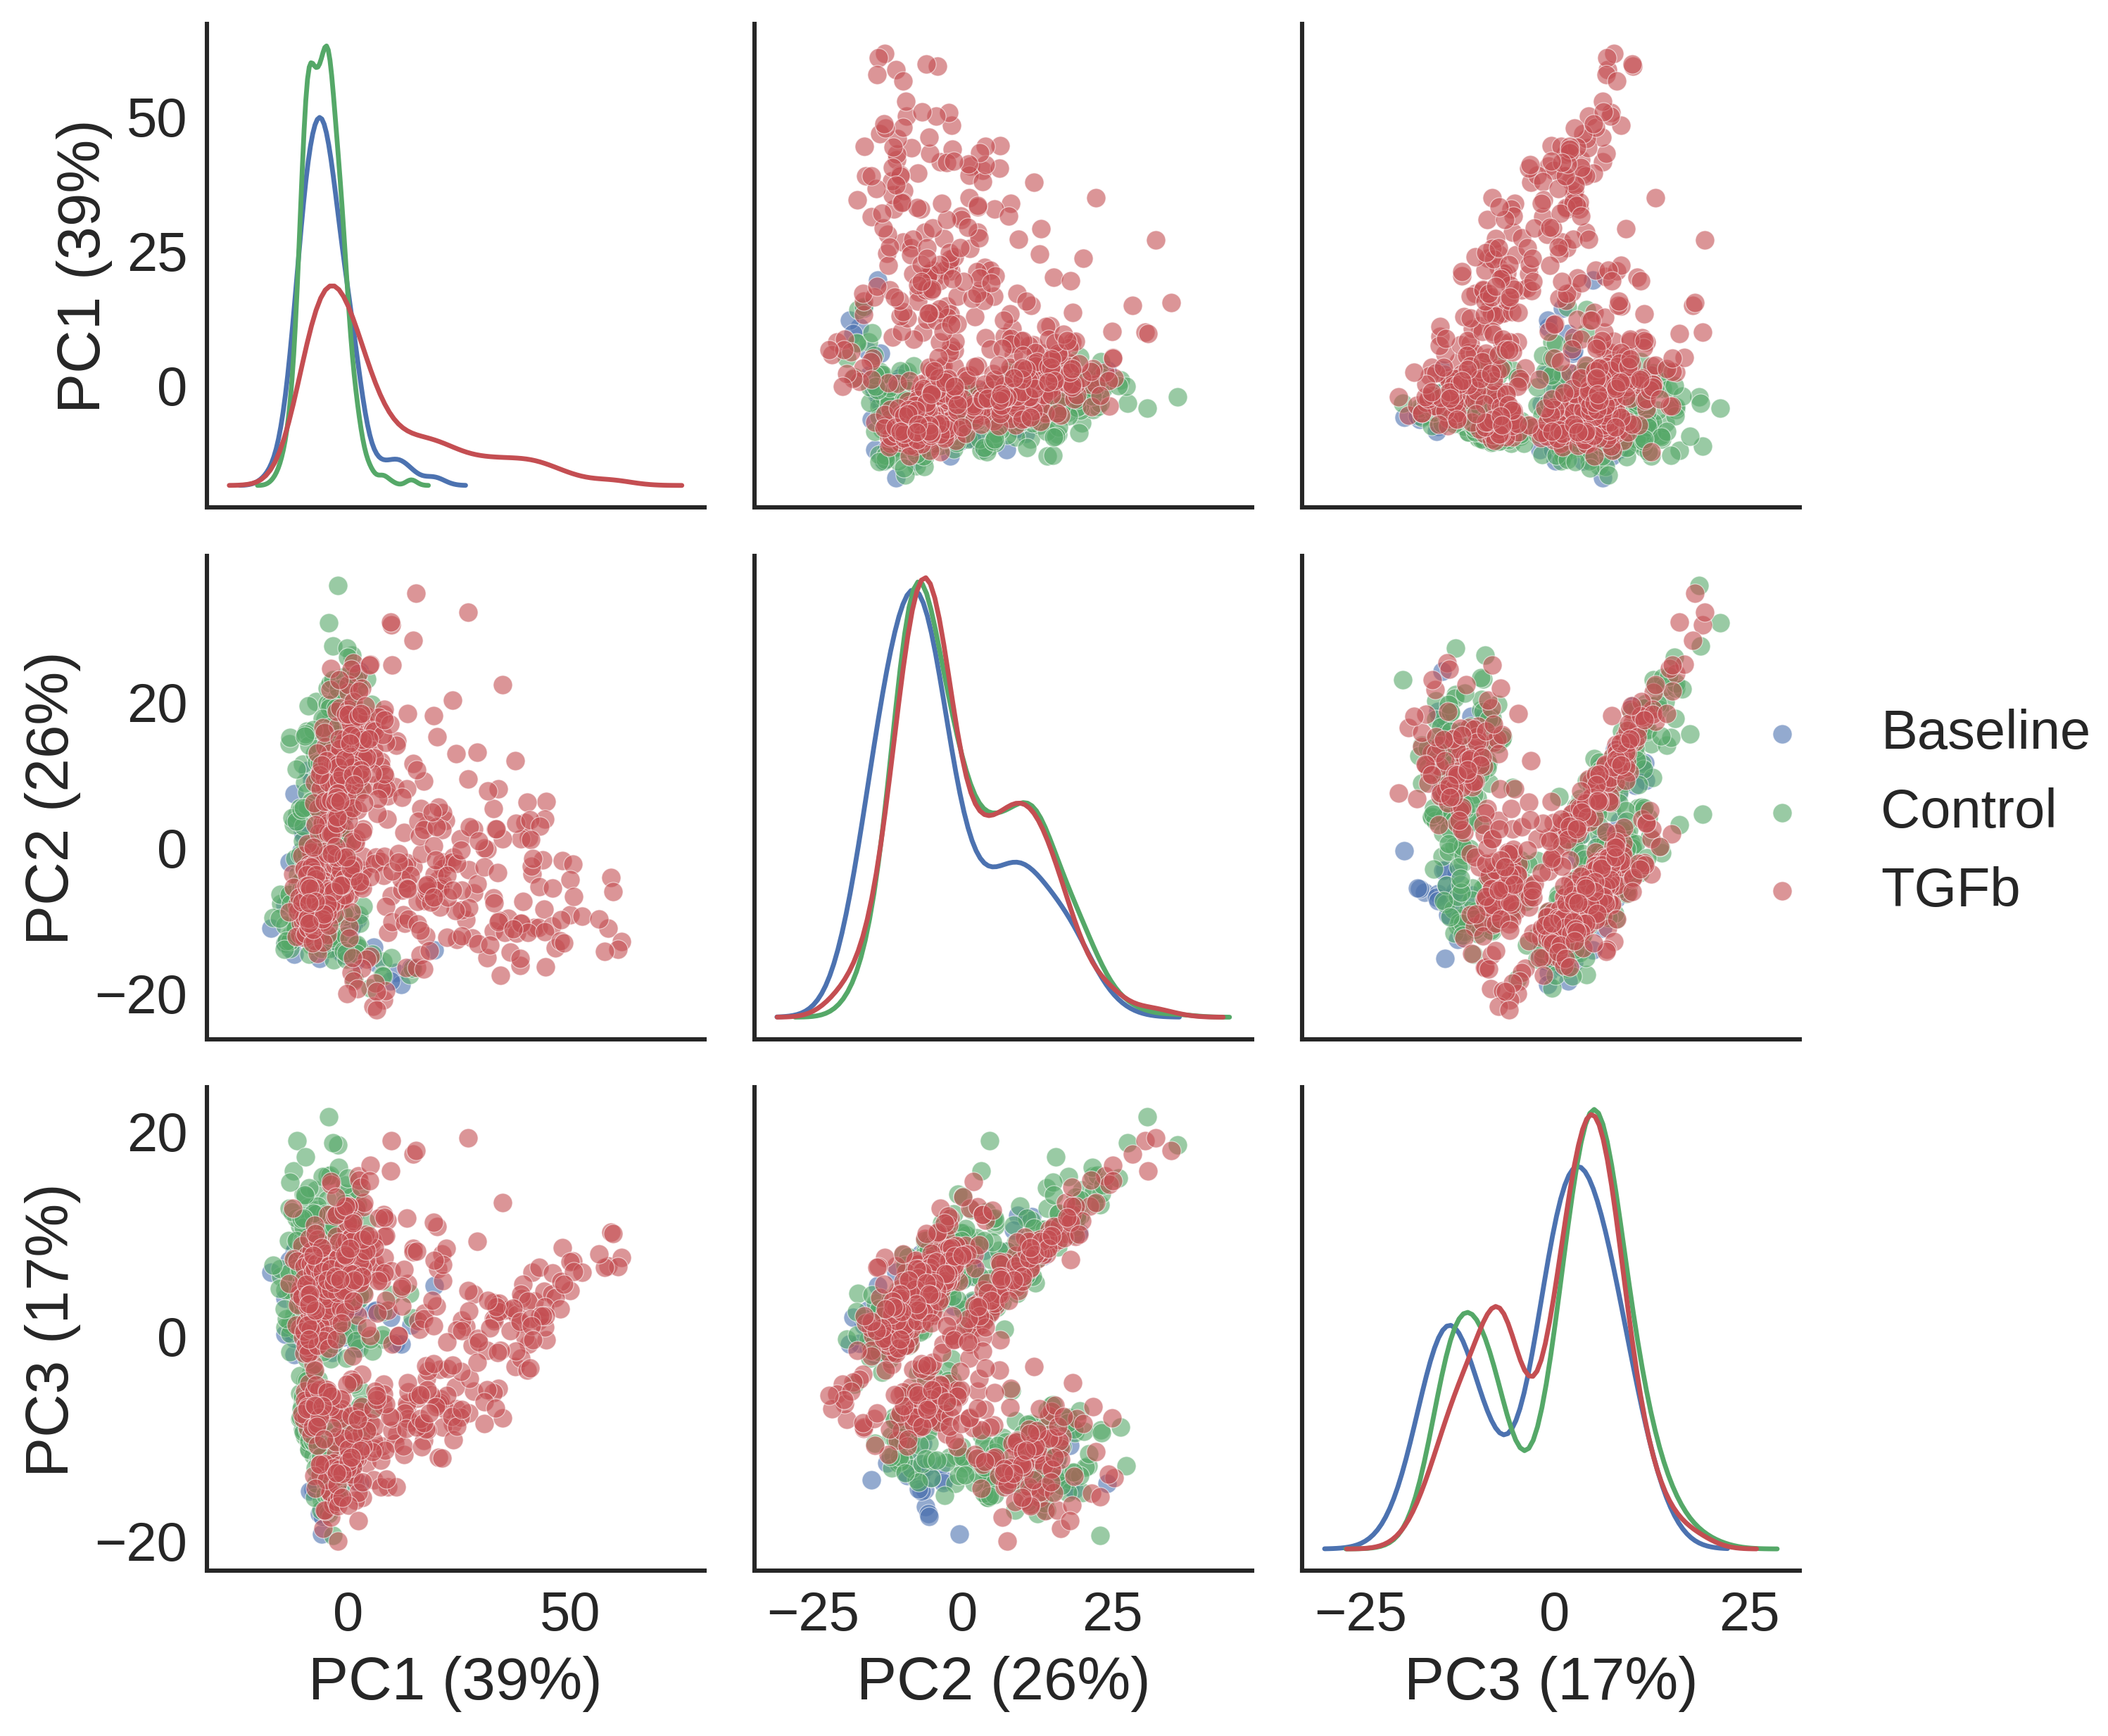
\includegraphics[height=0.45\textheight]{img/qc/treatment}
	\caption{Scatter matrix of first three principle components coloured by treatment.}
	\label{fig:qc:treatment}
\end{figure}

\begin{figure}
	\centering
	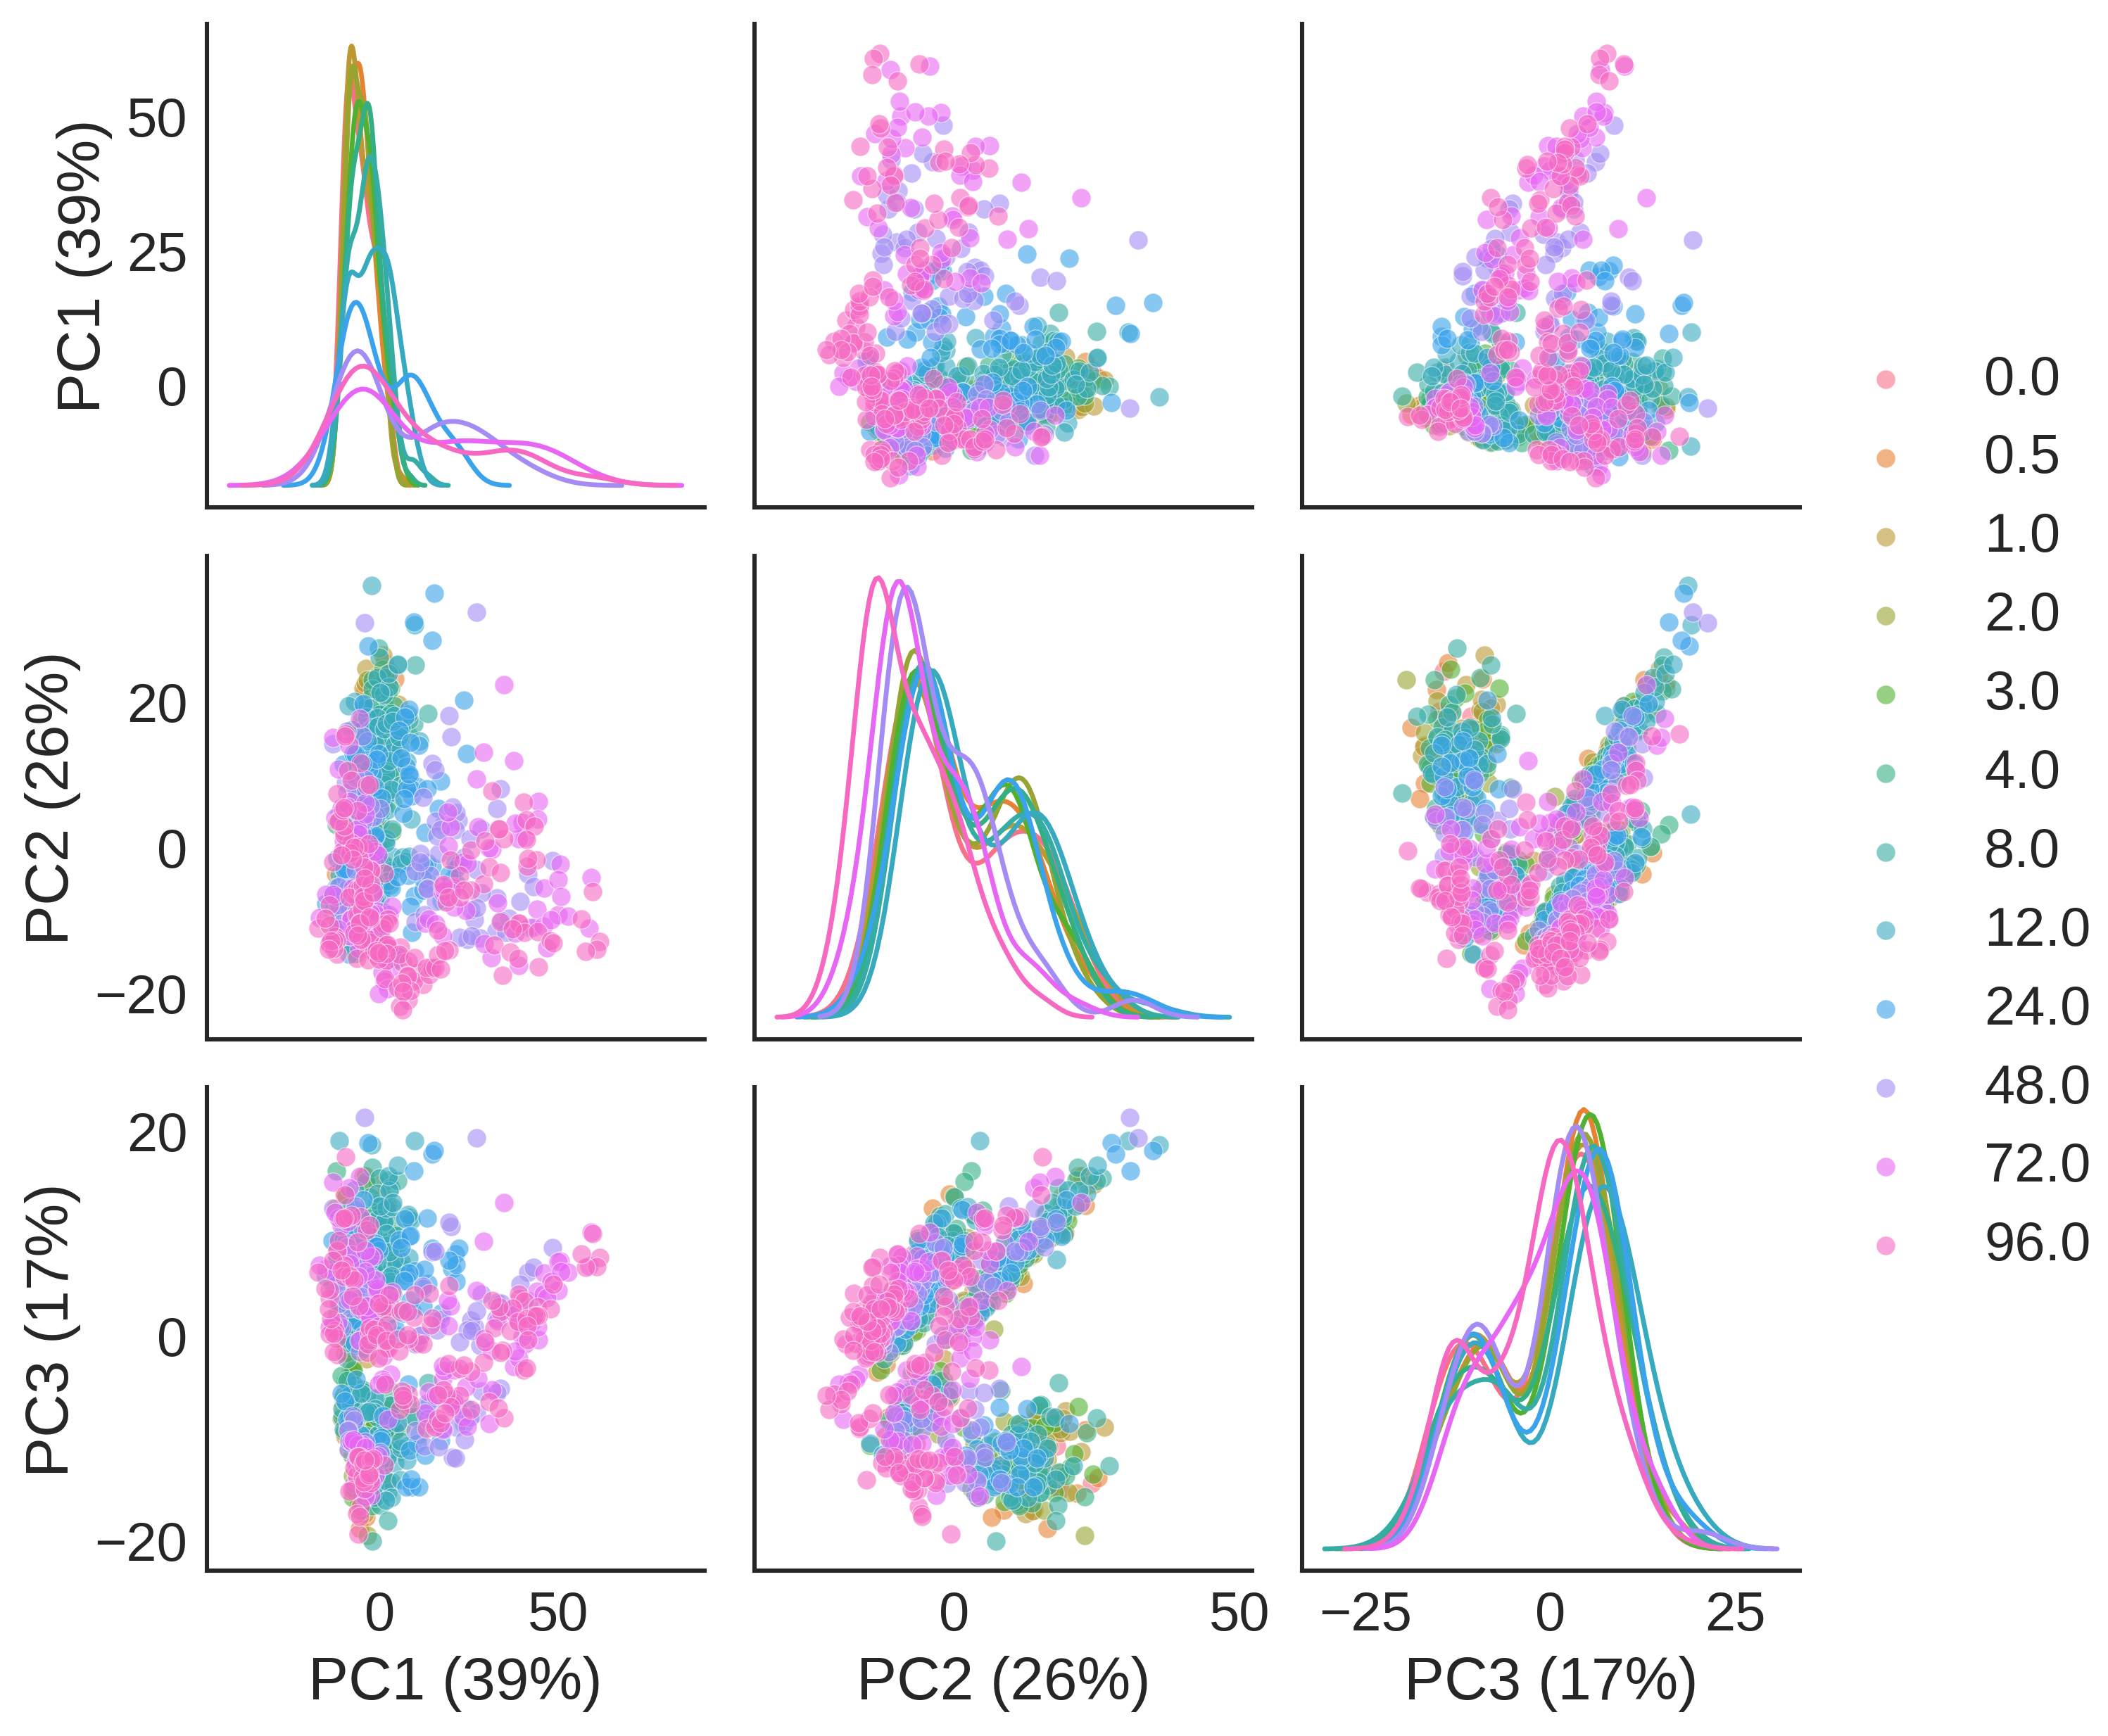
\includegraphics[height=0.45\textheight]{img/qc/time_point}
	\caption{Scatter matrix of first three principle components coloured by time point.}
	\label{fig:qc:time_point}
\end{figure}

\begin{figure}
	\centering
	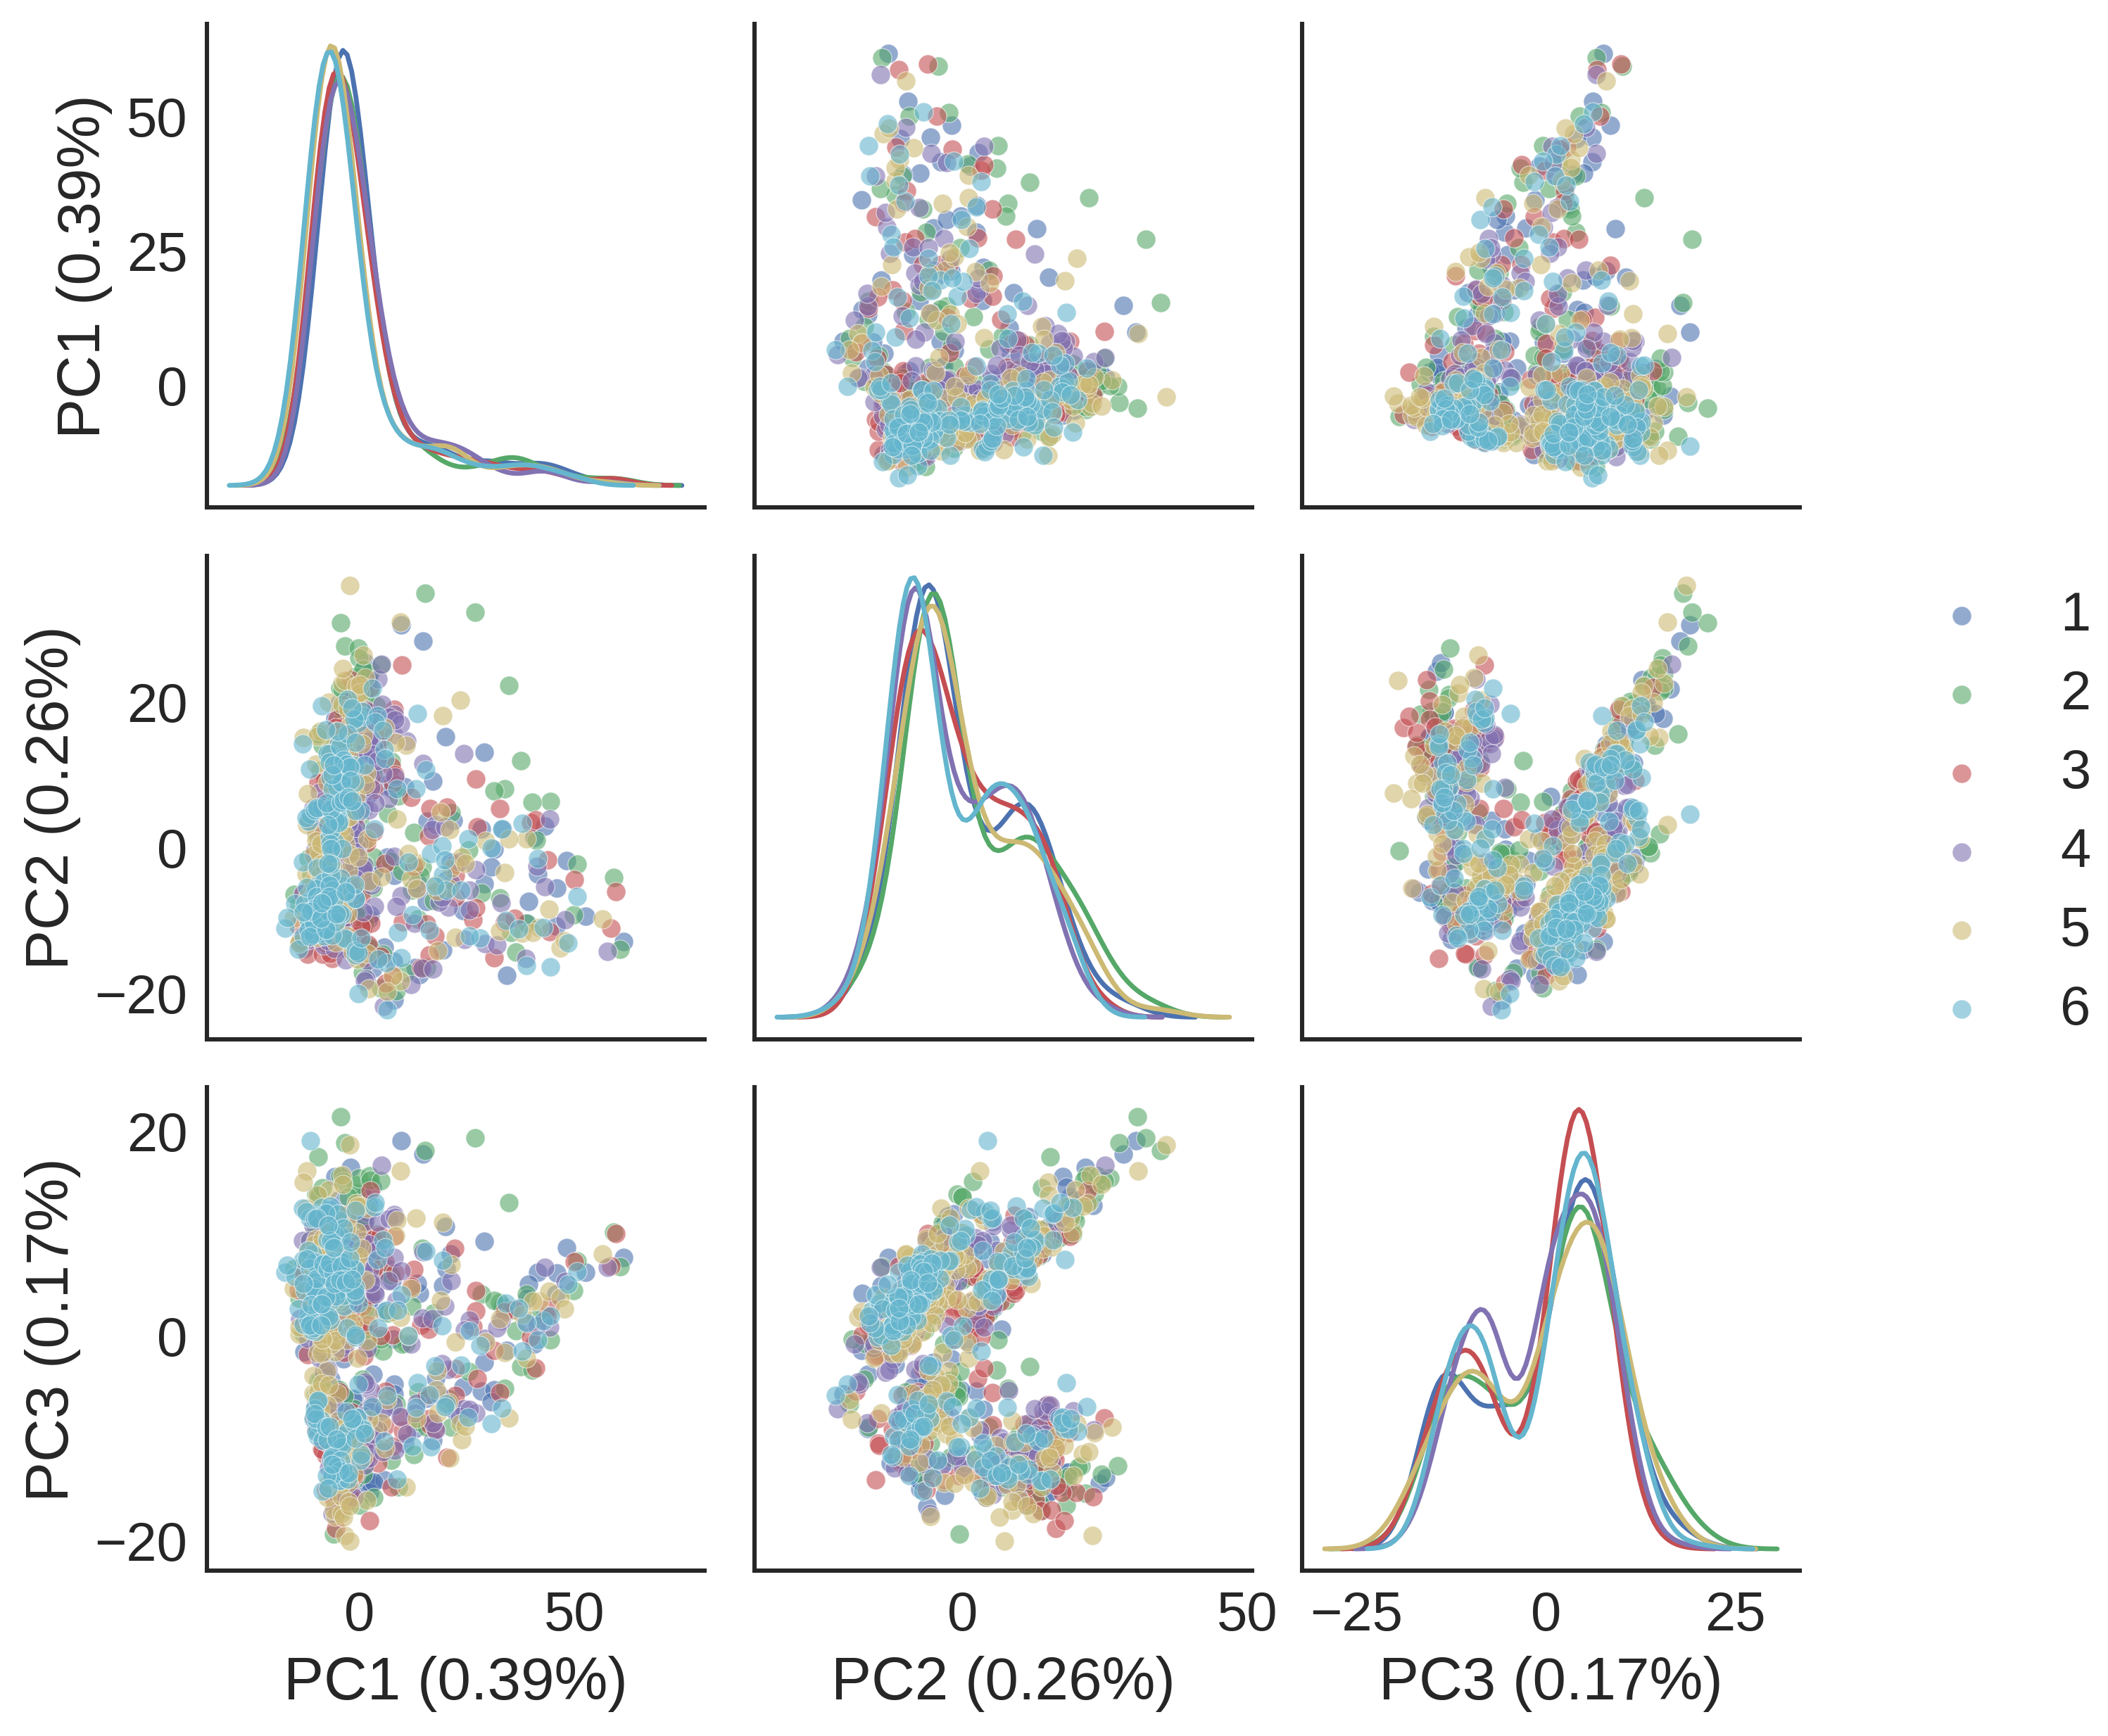
\includegraphics[height=0.45\textheight]{img/qc/replicate}
	\caption{Scatter matrix of first three principle components coloured by replicate.}
	\label{fig:qc:replicate}
\end{figure}

%While 72 genes is by no means a comprehensive accounting of the potential differences between these cell lines, these genes were selected based on their known involvement in ECM and \tgf{} biology. It is clear from the PCA that we have observed marked differences in the behaviour of neonatal, adult and senescent cells \cref{fig:qc:cell_line}. Additionally, the PCA serves to confirm that cells treated with \tgf{} behave differently to those treated with a negative control (\cref{fig:qc:treatment} an that the longer cells are treated, the more different they become, compared to baseline and control samples (\cref{fig:qc:time_point}. Moreover, the PCA does indicate replicate clustering which would be indicative of a confounding factor affecting the results \cref{fig:qc:replicate}.

%While PCA was used to provide an overview of the data, a differential expression analysis was used to compare full time series data between conditions. The main goal of the differential expression analysis was to provide statistical support for the existence of different behaviour between adult/senescent and neonatal fibroblasts.  Because considerable heterogeneity is known to exist between in the ageing process, we decided repeat the experiment times with three individuals per group. This enables a secondary goal of comparing individuals within a group to identify within group variability. To make use of the available data, all relevant combinations of `between' and `within' group comparisons were made for both \tgf{} and control treatments (\cref{fig:stats:diagram}). The results of these differential expression analyses were aggregated by calculating the proportion of the time a gene was differentially expressed at an FDR adjusted p-value less than 0.001. As an example of interpretation, \cref{fig:between_heatmap} shows that COL1A2 was differentially expressed in 100\% of possible comparisons (9) between \tgf{} treated adult and neonatal cell lines while COL1A2 was only differentially expressed in approximately 80\% of the comparisons between \tgf{} treated senescent and neonatal cell lines. 

%A summary of these comparisons is presented in \cref{table:stats_summary}, counting the number of genes that were differentially expressed in >60\% of differential expression analyses. It is interesting to note that more genes were differentially expressed in the \tgf{} time series data compared to the control time series data. Moreover, the comparison between adult and neonatal cell lines were the most different from each other while the comparison between neonatal cell lines and other neonatal cell lines in the control group were least different from each other. These statistics support the familiar notion that variability in gene expression is an increasing function of age. 
%\begin{figure}
%	\centering
%	\begin{subfigure}{0.25\linewidth}
%		
\includegraphics[width=\linewidth]{img/stats_diagram/between_adult}
%		\caption{Adult Vs neonatal}
%		%		\label{fig:diag:b}
%	\end{subfigure}\qquad
%	\begin{subfigure}{0.25\linewidth}
%		
\includegraphics[width=\linewidth]{img/stats_diagram/between_sen}
%		\caption{Senescent Vs neonatal}
%		%		\label{key}
%	\end{subfigure}
%	
%	\begin{subfigure}{0.15\linewidth}
%		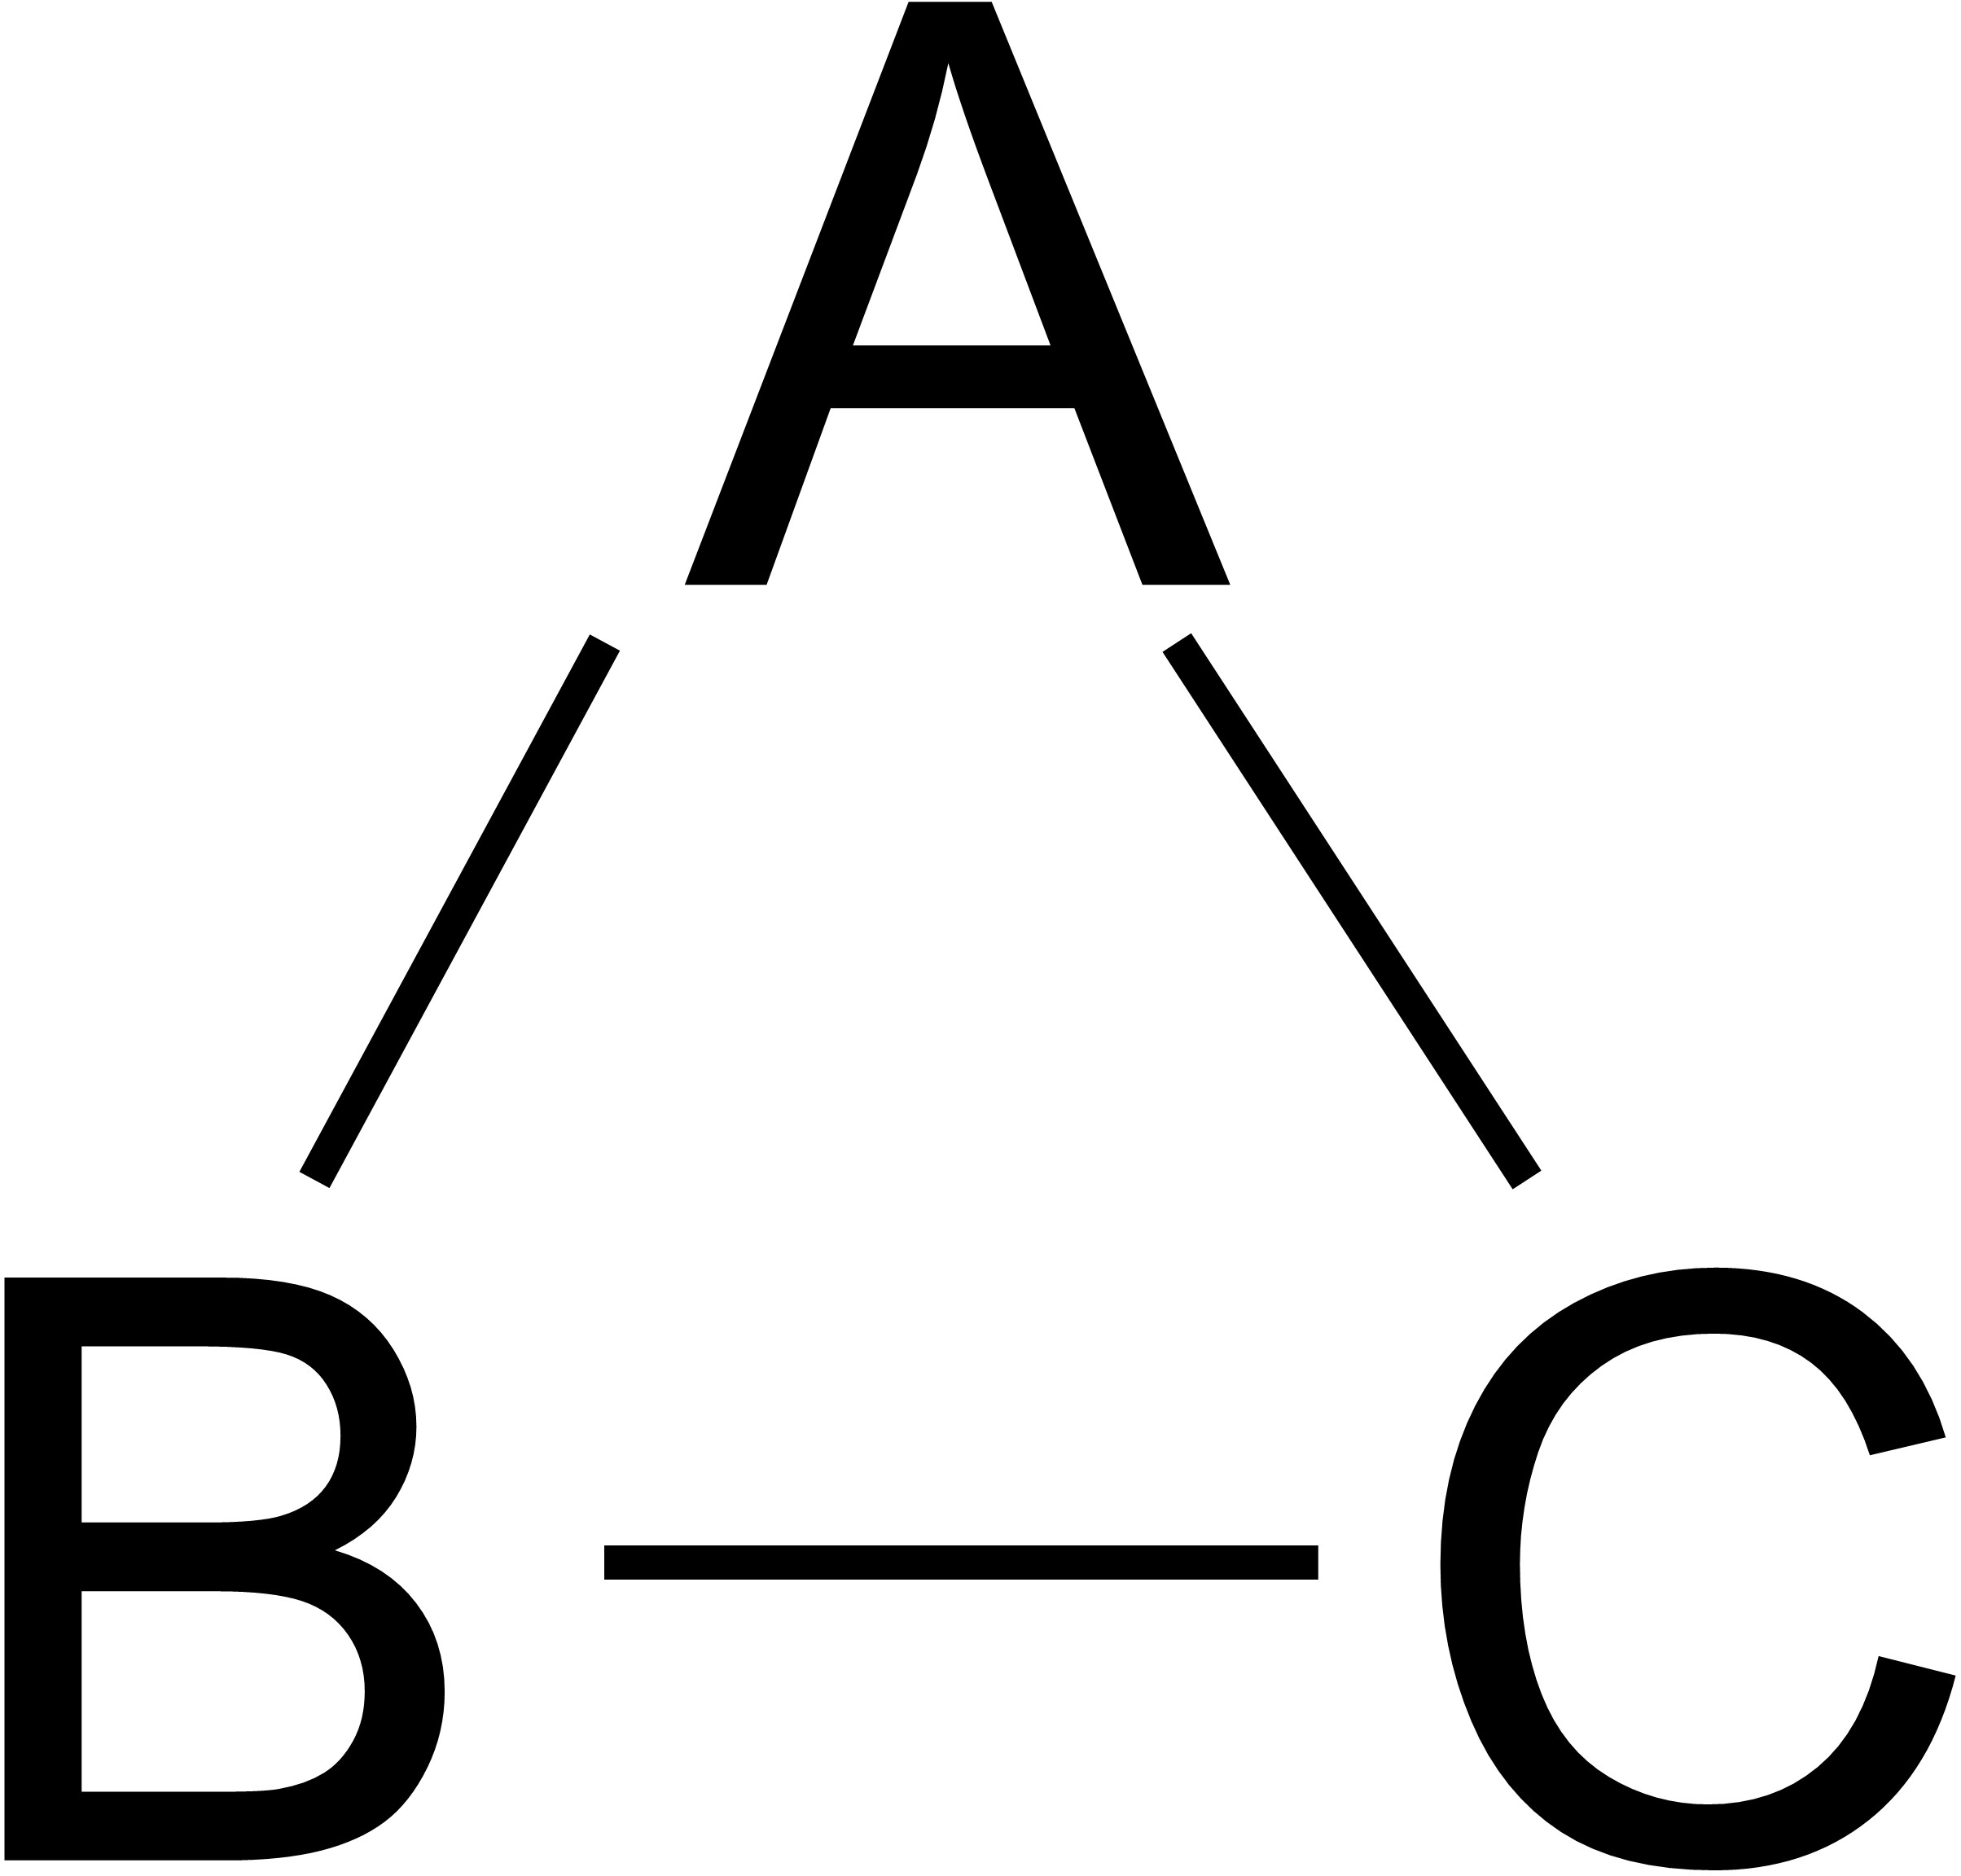
\includegraphics[width=\linewidth]{img/stats_diagram/within_neonatal}
%		\caption{Neonatal}
%		%		\label{key}
%	\end{subfigure}\qquad
%	\begin{subfigure}{0.125\linewidth}
%		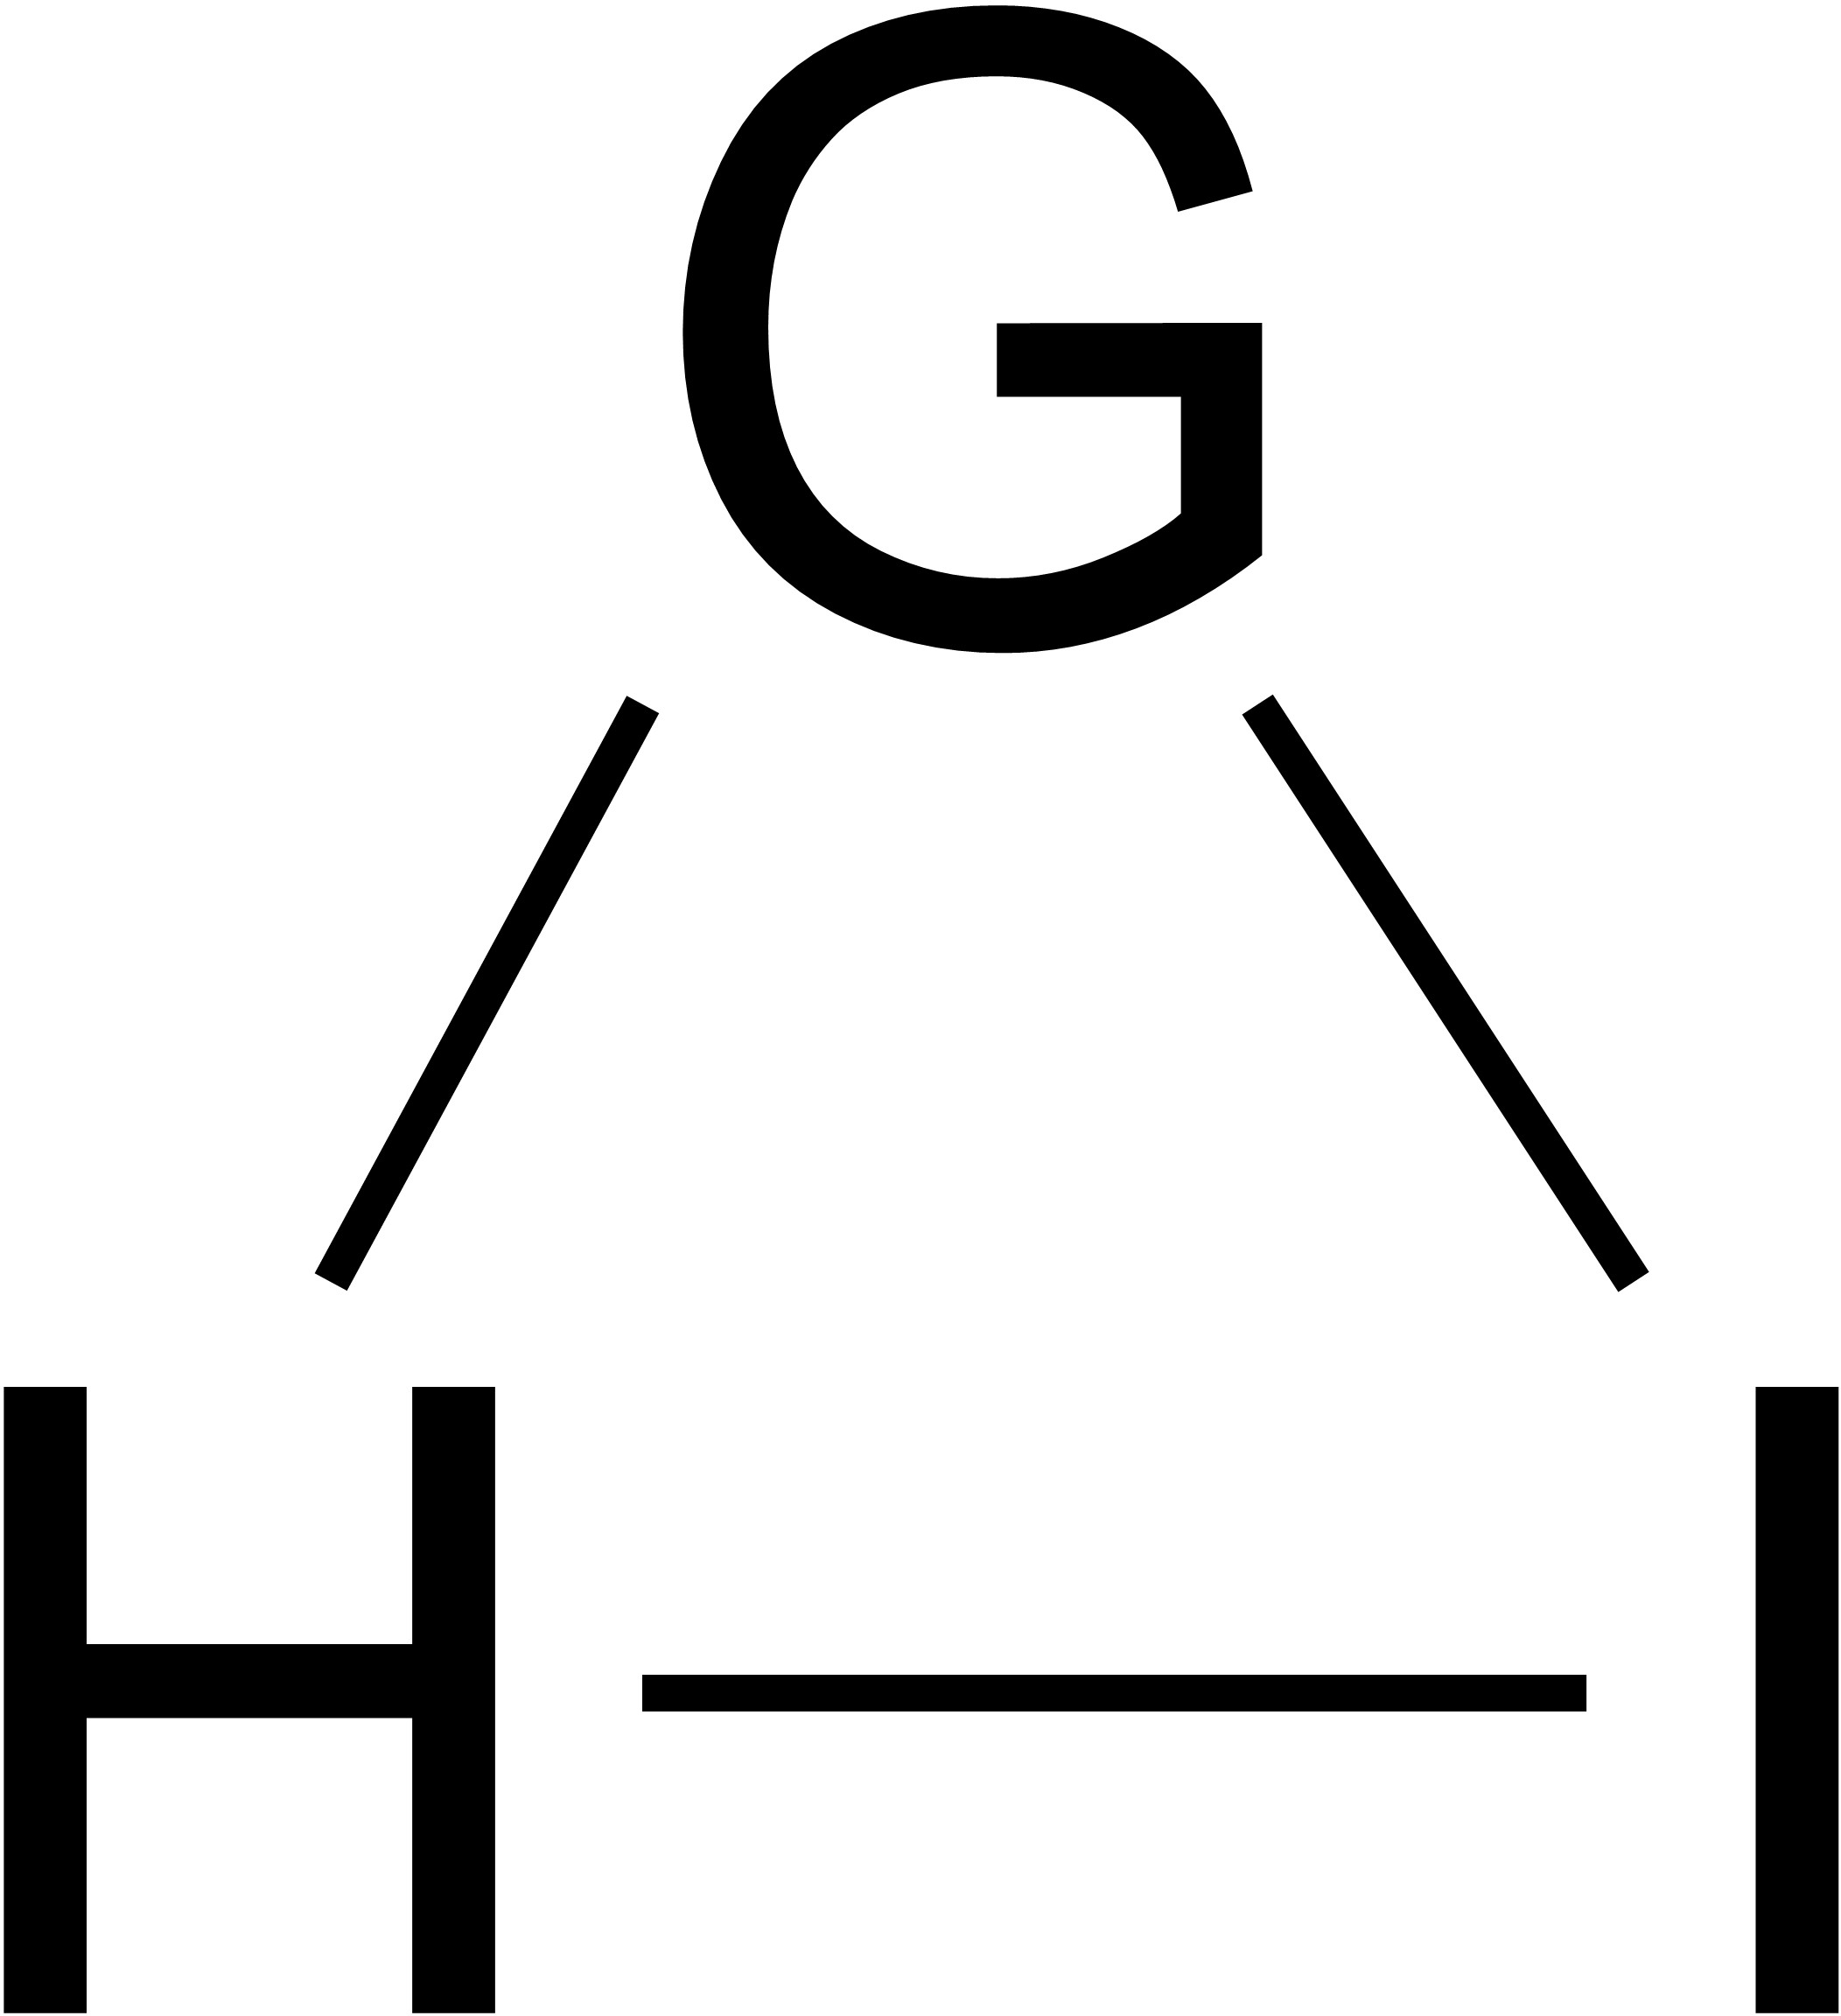
\includegraphics[width=\linewidth]{img/stats_diagram/within_adult}
%		\caption{Adult}
%		%		\label{key}
%	\end{subfigure}\qquad
%	\begin{subfigure}{0.15\linewidth}
%		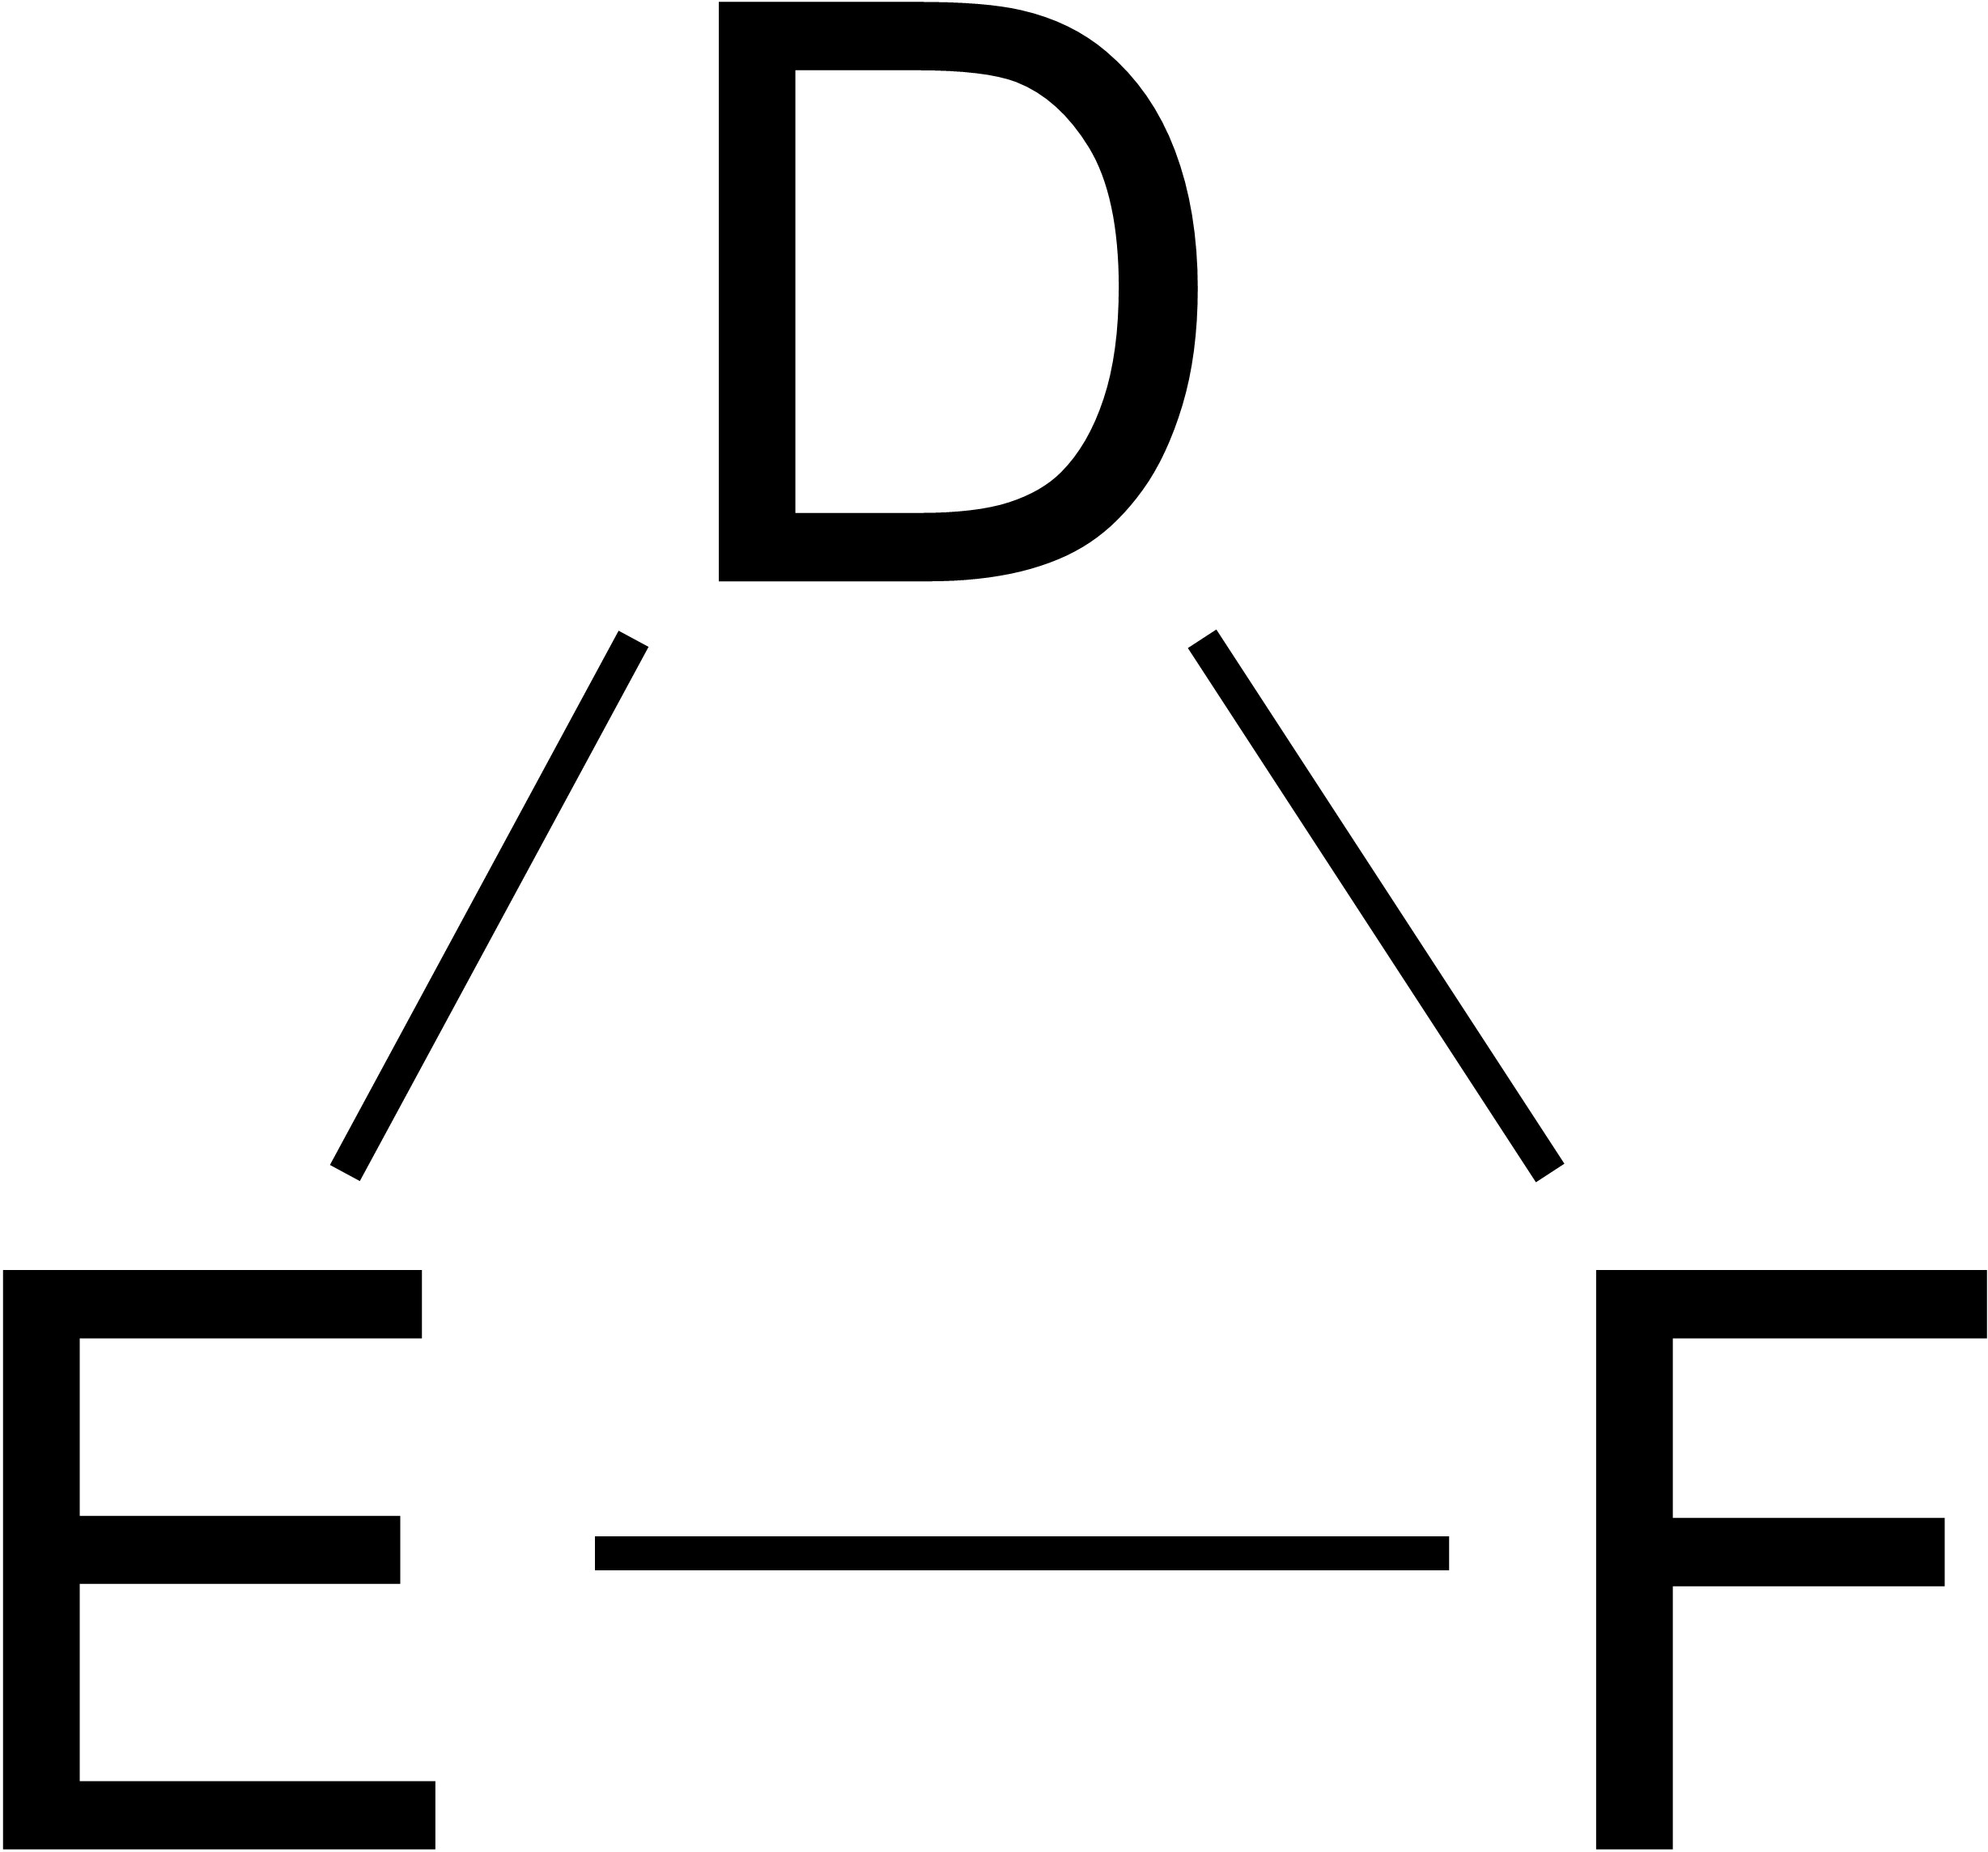
\includegraphics[width=\linewidth]{img/stats_diagram/within_senescent}
%		\caption{Senescent}
%	\end{subfigure}
%	\caption{Diagrammatic representation of comparisons made using LIMMA. Letters represent a cell ID while an edge signifies that a LIMMA analysis was conducted between the two. LIMMA analyses were conducted between (a) adult and neonatal and (b) senescent and neonatal. LIMMA analyses were also conducted within (c) neonatal (d) adult and (e) senescent cell lines. All differential expression analyses were conducted using LIMMA's spline method to compare full time series datasets.}
%	\label{fig:stats:diagram}
%\end{figure}
\end{document}
